\documentclass[twoside]{book}

% Packages required by doxygen
\usepackage{calc}
\usepackage{doxygen}
\usepackage{graphicx}
\usepackage[utf8]{inputenc}
\usepackage{makeidx}
\usepackage{multicol}
\usepackage{multirow}
\usepackage{textcomp}
\usepackage[table]{xcolor}

% Font selection
\usepackage[T1]{fontenc}
\usepackage{mathptmx}
\usepackage[scaled=.90]{helvet}
\usepackage{courier}
\usepackage{amssymb}
\usepackage{sectsty}
\renewcommand{\familydefault}{\sfdefault}
\allsectionsfont{%
  \fontseries{bc}\selectfont%
  \color{darkgray}%
}
\renewcommand{\DoxyLabelFont}{%
  \fontseries{bc}\selectfont%
  \color{darkgray}%
}

% Page & text layout
\usepackage{geometry}
\geometry{%
  a4paper,%
  top=2.5cm,%
  bottom=2.5cm,%
  left=2.5cm,%
  right=2.5cm%
}
\tolerance=750
\hfuzz=15pt
\hbadness=750
\setlength{\emergencystretch}{15pt}
\setlength{\parindent}{0cm}
\setlength{\parskip}{0.2cm}
\makeatletter
\renewcommand{\paragraph}{%
  \@startsection{paragraph}{4}{0ex}{-1.0ex}{1.0ex}{%
    \normalfont\normalsize\bfseries\SS@parafont%
  }%
}
\renewcommand{\subparagraph}{%
  \@startsection{subparagraph}{5}{0ex}{-1.0ex}{1.0ex}{%
    \normalfont\normalsize\bfseries\SS@subparafont%
  }%
}
\makeatother

% Headers & footers
\usepackage{fancyhdr}
\pagestyle{fancyplain}
\fancyhead[LE]{\fancyplain{}{\bfseries\thepage}}
\fancyhead[CE]{\fancyplain{}{}}
\fancyhead[RE]{\fancyplain{}{\bfseries\leftmark}}
\fancyhead[LO]{\fancyplain{}{\bfseries\rightmark}}
\fancyhead[CO]{\fancyplain{}{}}
\fancyhead[RO]{\fancyplain{}{\bfseries\thepage}}
\fancyfoot[LE]{\fancyplain{}{}}
\fancyfoot[CE]{\fancyplain{}{}}
\fancyfoot[RE]{\fancyplain{}{\bfseries\scriptsize Generated on Sun Dec 9 2018 18\-:38\-:00 for My Project by Doxygen }}
\fancyfoot[LO]{\fancyplain{}{\bfseries\scriptsize Generated on Sun Dec 9 2018 18\-:38\-:00 for My Project by Doxygen }}
\fancyfoot[CO]{\fancyplain{}{}}
\fancyfoot[RO]{\fancyplain{}{}}
\renewcommand{\footrulewidth}{0.4pt}
\renewcommand{\chaptermark}[1]{%
  \markboth{#1}{}%
}
\renewcommand{\sectionmark}[1]{%
  \markright{\thesection\ #1}%
}

% Indices & bibliography
\usepackage{natbib}
\usepackage[titles]{tocloft}
\setcounter{tocdepth}{3}
\setcounter{secnumdepth}{5}
\makeindex

% Hyperlinks (required, but should be loaded last)
\usepackage{ifpdf}
\ifpdf
  \usepackage[pdftex,pagebackref=true]{hyperref}
\else
  \usepackage[ps2pdf,pagebackref=true]{hyperref}
\fi
\hypersetup{%
  colorlinks=true,%
  linkcolor=blue,%
  citecolor=blue,%
  unicode%
}

% Custom commands
\newcommand{\clearemptydoublepage}{%
  \newpage{\pagestyle{empty}\cleardoublepage}%
}


%===== C O N T E N T S =====

\begin{document}

% Titlepage & ToC
\hypersetup{pageanchor=false}
\pagenumbering{roman}
\begin{titlepage}
\vspace*{7cm}
\begin{center}%
{\Large My Project }\\
\vspace*{1cm}
{\large Generated by Doxygen 1.8.6}\\
\vspace*{0.5cm}
{\small Sun Dec 9 2018 18:38:00}\\
\end{center}
\end{titlepage}
\clearemptydoublepage
\tableofcontents
\clearemptydoublepage
\pagenumbering{arabic}
\hypersetup{pageanchor=true}

%--- Begin generated contents ---
\chapter{E\-E\-C\-E435\-L Game}
\label{index}\hypertarget{index}{}A game containing two sub-\/games designed to help kids learn programming \begin{DoxyAuthor}{Author}
Ali Al Akbar Haidoura 

Camille farhat 
\end{DoxyAuthor}
\begin{DoxyDate}{Date}
9-\/12-\/2018 
\end{DoxyDate}

\chapter{Hierarchical Index}
\section{Class Hierarchy}
This inheritance list is sorted roughly, but not completely, alphabetically\-:\begin{DoxyCompactList}
\item \contentsline{section}{Level\-Parser}{\pageref{classLevelParser}}{}
\item \contentsline{section}{levels}{\pageref{classlevels}}{}
\item Q\-Graphics\-Pixmap\-Item\begin{DoxyCompactList}
\item \contentsline{section}{boat}{\pageref{classboat}}{}
\item \contentsline{section}{Bug}{\pageref{classBug}}{}
\item \contentsline{section}{Bullet}{\pageref{classBullet}}{}
\item \contentsline{section}{Coffee\-Cup}{\pageref{classCoffeeCup}}{}
\item \contentsline{section}{Life\-Counter}{\pageref{classLifeCounter}}{}
\item \contentsline{section}{locks}{\pageref{classlocks}}{}
\item \contentsline{section}{mini\-Bug}{\pageref{classminiBug}}{}
\item \contentsline{section}{Popeye}{\pageref{classPopeye}}{}
\item \contentsline{section}{Quality\-Control\-Icon}{\pageref{classQualityControlIcon}}{}
\item \contentsline{section}{river}{\pageref{classriver}}{}
\item \contentsline{section}{river\-Obstacle}{\pageref{classriverObstacle}}{}
\item \contentsline{section}{rock}{\pageref{classrock}}{}
\item \contentsline{section}{Shield}{\pageref{classShield}}{}
\item \contentsline{section}{small\-River}{\pageref{classsmallRiver}}{}
\item \contentsline{section}{spinach}{\pageref{classspinach}}{}
\item \contentsline{section}{Tester}{\pageref{classTester}}{}
\item \contentsline{section}{Testing\-Icon}{\pageref{classTestingIcon}}{}
\item \contentsline{section}{Wall}{\pageref{classWall}}{}
\end{DoxyCompactList}
\item Q\-Graphics\-Scene\begin{DoxyCompactList}
\item \contentsline{section}{game1scene}{\pageref{classgame1scene}}{}
\item \contentsline{section}{Game2\-Scene}{\pageref{classGame2Scene}}{}
\item \contentsline{section}{levelsscene}{\pageref{classlevelsscene}}{}
\end{DoxyCompactList}
\item Q\-Object\begin{DoxyCompactList}
\item \contentsline{section}{boat}{\pageref{classboat}}{}
\item \contentsline{section}{Bug}{\pageref{classBug}}{}
\item \contentsline{section}{Bullet}{\pageref{classBullet}}{}
\item \contentsline{section}{locks}{\pageref{classlocks}}{}
\item \contentsline{section}{mini\-Bug}{\pageref{classminiBug}}{}
\item \contentsline{section}{Popeye}{\pageref{classPopeye}}{}
\item \contentsline{section}{river}{\pageref{classriver}}{}
\item \contentsline{section}{river\-Obstacle}{\pageref{classriverObstacle}}{}
\item \contentsline{section}{rock}{\pageref{classrock}}{}
\item \contentsline{section}{small\-River}{\pageref{classsmallRiver}}{}
\item \contentsline{section}{spinach}{\pageref{classspinach}}{}
\item \contentsline{section}{Tester}{\pageref{classTester}}{}
\item \contentsline{section}{Testing\-Icon}{\pageref{classTestingIcon}}{}
\end{DoxyCompactList}
\item Q\-Widget\begin{DoxyCompactList}
\item \contentsline{section}{game\-Over}{\pageref{classgameOver}}{}
\item \contentsline{section}{games\-Widget}{\pageref{classgamesWidget}}{}
\item \contentsline{section}{hints}{\pageref{classhints}}{}
\item \contentsline{section}{instruction}{\pageref{classinstruction}}{}
\item \contentsline{section}{logg\-In\-Widget}{\pageref{classloggInWidget}}{}
\item \contentsline{section}{Log\-On\-Widget}{\pageref{classLogOnWidget}}{}
\item \contentsline{section}{lost}{\pageref{classlost}}{}
\item \contentsline{section}{sign\-In\-Widget}{\pageref{classsignInWidget}}{}
\item \contentsline{section}{Sign\-Up\-Widget}{\pageref{classSignUpWidget}}{}
\item \contentsline{section}{Won}{\pageref{classWon}}{}
\end{DoxyCompactList}
\end{DoxyCompactList}

\chapter{Class Index}
\section{Class List}
Here are the classes, structs, unions and interfaces with brief descriptions\-:\begin{DoxyCompactList}
\item\contentsline{section}{\hyperlink{classboat}{boat} }{\pageref{classboat}}{}
\item\contentsline{section}{\hyperlink{classBug}{Bug} }{\pageref{classBug}}{}
\item\contentsline{section}{\hyperlink{classBullet}{Bullet} }{\pageref{classBullet}}{}
\item\contentsline{section}{\hyperlink{classCoffeeCup}{Coffee\-Cup} }{\pageref{classCoffeeCup}}{}
\item\contentsline{section}{\hyperlink{classgame1scene}{game1scene} }{\pageref{classgame1scene}}{}
\item\contentsline{section}{\hyperlink{classGame2Scene}{Game2\-Scene} }{\pageref{classGame2Scene}}{}
\item\contentsline{section}{\hyperlink{classgameOver}{game\-Over} }{\pageref{classgameOver}}{}
\item\contentsline{section}{\hyperlink{classgamesWidget}{games\-Widget} }{\pageref{classgamesWidget}}{}
\item\contentsline{section}{\hyperlink{classhints}{hints} }{\pageref{classhints}}{}
\item\contentsline{section}{\hyperlink{classinstruction}{instruction} }{\pageref{classinstruction}}{}
\item\contentsline{section}{\hyperlink{classLevelParser}{Level\-Parser} }{\pageref{classLevelParser}}{}
\item\contentsline{section}{\hyperlink{classlevels}{levels} }{\pageref{classlevels}}{}
\item\contentsline{section}{\hyperlink{classlevelsscene}{levelsscene} }{\pageref{classlevelsscene}}{}
\item\contentsline{section}{\hyperlink{classLifeCounter}{Life\-Counter} }{\pageref{classLifeCounter}}{}
\item\contentsline{section}{\hyperlink{classlocks}{locks} }{\pageref{classlocks}}{}
\item\contentsline{section}{\hyperlink{classloggInWidget}{logg\-In\-Widget} }{\pageref{classloggInWidget}}{}
\item\contentsline{section}{\hyperlink{classLogOnWidget}{Log\-On\-Widget} }{\pageref{classLogOnWidget}}{}
\item\contentsline{section}{\hyperlink{classlost}{lost} }{\pageref{classlost}}{}
\item\contentsline{section}{\hyperlink{classminiBug}{mini\-Bug} }{\pageref{classminiBug}}{}
\item\contentsline{section}{\hyperlink{classPopeye}{Popeye} }{\pageref{classPopeye}}{}
\item\contentsline{section}{\hyperlink{classQualityControlIcon}{Quality\-Control\-Icon} }{\pageref{classQualityControlIcon}}{}
\item\contentsline{section}{\hyperlink{classriver}{river} }{\pageref{classriver}}{}
\item\contentsline{section}{\hyperlink{classriverObstacle}{river\-Obstacle} }{\pageref{classriverObstacle}}{}
\item\contentsline{section}{\hyperlink{classrock}{rock} }{\pageref{classrock}}{}
\item\contentsline{section}{\hyperlink{classShield}{Shield} }{\pageref{classShield}}{}
\item\contentsline{section}{\hyperlink{classsignInWidget}{sign\-In\-Widget} }{\pageref{classsignInWidget}}{}
\item\contentsline{section}{\hyperlink{classSignUpWidget}{Sign\-Up\-Widget} }{\pageref{classSignUpWidget}}{}
\item\contentsline{section}{\hyperlink{classsmallRiver}{small\-River} }{\pageref{classsmallRiver}}{}
\item\contentsline{section}{\hyperlink{classspinach}{spinach} }{\pageref{classspinach}}{}
\item\contentsline{section}{\hyperlink{classTester}{Tester} }{\pageref{classTester}}{}
\item\contentsline{section}{\hyperlink{classTestingIcon}{Testing\-Icon} }{\pageref{classTestingIcon}}{}
\item\contentsline{section}{\hyperlink{classWall}{Wall} }{\pageref{classWall}}{}
\item\contentsline{section}{\hyperlink{classWon}{Won} }{\pageref{classWon}}{}
\end{DoxyCompactList}

\chapter{File Index}
\section{File List}
Here is a list of all documented files with brief descriptions\-:\begin{DoxyCompactList}
\item\contentsline{section}{\hyperlink{boat_8cpp}{boat.\-cpp} \\*Contains \hyperlink{classPopeye}{Popeye} class definition }{\pageref{boat_8cpp}}{}
\item\contentsline{section}{\hyperlink{boat_8h}{boat.\-h} \\*Boat class definition }{\pageref{boat_8h}}{}
\item\contentsline{section}{\hyperlink{bug_8cpp}{bug.\-cpp} \\*\hyperlink{classBug}{Bug} class definitions }{\pageref{bug_8cpp}}{}
\item\contentsline{section}{\hyperlink{bug_8h}{bug.\-h} \\*Q\-Graphics\-Pixmap\-Item representing the bugs }{\pageref{bug_8h}}{}
\item\contentsline{section}{\hyperlink{bullet_8cpp}{bullet.\-cpp} \\*\hyperlink{classBullet}{Bullet} class definitions }{\pageref{bullet_8cpp}}{}
\item\contentsline{section}{\hyperlink{bullet_8h}{bullet.\-h} \\*Q\-Graphics\-Pixmap\-Item representing the bullets }{\pageref{bullet_8h}}{}
\item\contentsline{section}{\hyperlink{coffeecup_8cpp}{coffeecup.\-cpp} \\*Contains \hyperlink{classCoffeeCup}{Coffee\-Cup} Class definitions }{\pageref{coffeecup_8cpp}}{}
\item\contentsline{section}{\hyperlink{coffeecup_8h}{coffeecup.\-h} \\*Q\-Graphics\-Pixmap\-Item representing the Coffee Cup }{\pageref{coffeecup_8h}}{}
\item\contentsline{section}{\hyperlink{game1scene_8cpp}{game1scene.\-cpp} \\*Game1's class definition }{\pageref{game1scene_8cpp}}{}
\item\contentsline{section}{\hyperlink{game1scene_8h}{game1scene.\-h} \\*The Game's scene }{\pageref{game1scene_8h}}{}
\item\contentsline{section}{\hyperlink{game2scene_8cpp}{game2scene.\-cpp} \\*Contains \hyperlink{classGame2Scene}{Game2\-Scene} Class definitions }{\pageref{game2scene_8cpp}}{}
\item\contentsline{section}{\hyperlink{game2scene_8h}{game2scene.\-h} \\*The scene in which all the logic and items of Game2 are located }{\pageref{game2scene_8h}}{}
\item\contentsline{section}{{\bfseries gameover.\-h} }{\pageref{gameover_8h}}{}
\item\contentsline{section}{\hyperlink{gameswidget_8cpp}{gameswidget.\-cpp} \\*Game1-\/2 Links }{\pageref{gameswidget_8cpp}}{}
\item\contentsline{section}{{\bfseries gameswidget.\-h} }{\pageref{gameswidget_8h}}{}
\item\contentsline{section}{\hyperlink{hints_8cpp}{hints.\-cpp} \\*Shows the appropriate hints in a pop up window }{\pageref{hints_8cpp}}{}
\item\contentsline{section}{\hyperlink{hints_8h}{hints.\-h} \\*The Level's scene's Hints }{\pageref{hints_8h}}{}
\item\contentsline{section}{\hyperlink{instruction_8cpp}{instruction.\-cpp} \\*Shows the initial instructions to start the game in a pop up window }{\pageref{instruction_8cpp}}{}
\item\contentsline{section}{\hyperlink{instruction_8h}{instruction.\-h} \\*The Level's scene's levels pop up used for displaying instructions }{\pageref{instruction_8h}}{}
\item\contentsline{section}{\hyperlink{levelparser_8cpp}{levelparser.\-cpp} \\*Contains \hyperlink{classLevelParser}{Level\-Parser} Class definitions }{\pageref{levelparser_8cpp}}{}
\item\contentsline{section}{\hyperlink{levelparser_8h}{levelparser.\-h} \\*Parses the game2 levels from the text files }{\pageref{levelparser_8h}}{}
\item\contentsline{section}{\hyperlink{levels_8cpp}{levels.\-cpp} \\*Setting up the different specs for each level to load them dynamically everytime a user starts a level }{\pageref{levels_8cpp}}{}
\item\contentsline{section}{\hyperlink{levels_8h}{levels.\-h} \\*The Level Object }{\pageref{levels_8h}}{}
\item\contentsline{section}{\hyperlink{levelsscene_8cpp}{levelsscene.\-cpp} \\*Contains Game1's class definition }{\pageref{levelsscene_8cpp}}{}
\item\contentsline{section}{{\bfseries levelsscene.\-h} }{\pageref{levelsscene_8h}}{}
\item\contentsline{section}{\hyperlink{lifecounter_8cpp}{lifecounter.\-cpp} \\*Contains \hyperlink{classLifeCounter}{Life\-Counter} Class definitions }{\pageref{lifecounter_8cpp}}{}
\item\contentsline{section}{\hyperlink{lifecounter_8h}{lifecounter.\-h} \\*Q\-Graphics\-Pixmap\-Item representing }{\pageref{lifecounter_8h}}{}
\item\contentsline{section}{\hyperlink{locks_8cpp}{locks.\-cpp} \\*Contains Lock class definition }{\pageref{locks_8cpp}}{}
\item\contentsline{section}{\hyperlink{locks_8h}{locks.\-h} \\*Contains Lock class definition }{\pageref{locks_8h}}{}
\item\contentsline{section}{{\bfseries logginwidget.\-h} }{\pageref{logginwidget_8h}}{}
\item\contentsline{section}{{\bfseries logonwidget.\-h} }{\pageref{logonwidget_8h}}{}
\item\contentsline{section}{\hyperlink{lost_8cpp}{lost.\-cpp} \\*Shows the appropriate loose message in a pop up window }{\pageref{lost_8cpp}}{}
\item\contentsline{section}{\hyperlink{lost_8h}{lost.\-h} \\*The Level's scene's loose pop up }{\pageref{lost_8h}}{}
\item\contentsline{section}{\hyperlink{minibug_8cpp}{minibug.\-cpp} \\*Contains \hyperlink{classminiBug}{mini\-Bug} Class definitions }{\pageref{minibug_8cpp}}{}
\item\contentsline{section}{{\bfseries minibug.\-h} }{\pageref{minibug_8h}}{}
\item\contentsline{section}{\hyperlink{popeye_8cpp}{popeye.\-cpp} \\*Contains \hyperlink{classPopeye}{Popeye} class definition }{\pageref{popeye_8cpp}}{}
\item\contentsline{section}{\hyperlink{popeye_8h}{popeye.\-h} \\*Contains \hyperlink{classPopeye}{Popeye} class definition }{\pageref{popeye_8h}}{}
\item\contentsline{section}{\hyperlink{qualitycontrolicon_8cpp}{qualitycontrolicon.\-cpp} \\*Contains \hyperlink{classQualityControlIcon}{Quality\-Control\-Icon} Class definitions }{\pageref{qualitycontrolicon_8cpp}}{}
\item\contentsline{section}{\hyperlink{qualitycontrolicon_8h}{qualitycontrolicon.\-h} \\*Q\-Graphics\-Pixmap\-Item representing the quality control icon }{\pageref{qualitycontrolicon_8h}}{}
\item\contentsline{section}{\hyperlink{river_8cpp}{river.\-cpp} \\*Contains river class definition }{\pageref{river_8cpp}}{}
\item\contentsline{section}{\hyperlink{river_8h}{river.\-h} \\*Contains \hyperlink{classPopeye}{Popeye} class definition }{\pageref{river_8h}}{}
\item\contentsline{section}{\hyperlink{riverobstacle_8cpp}{riverobstacle.\-cpp} \\*Contains River Obstacle class definition }{\pageref{riverobstacle_8cpp}}{}
\item\contentsline{section}{\hyperlink{riverobstacle_8h}{riverobstacle.\-h} \\*Contains River Obstacle class definition }{\pageref{riverobstacle_8h}}{}
\item\contentsline{section}{\hyperlink{rock_8cpp}{rock.\-cpp} \\*Rock class definition }{\pageref{rock_8cpp}}{}
\item\contentsline{section}{\hyperlink{rock_8h}{rock.\-h} \\*Rock class definition }{\pageref{rock_8h}}{}
\item\contentsline{section}{\hyperlink{shield_8cpp}{shield.\-cpp} \\*Contains shield Class definitions }{\pageref{shield_8cpp}}{}
\item\contentsline{section}{\hyperlink{shield_8h}{shield.\-h} \\*Q\-Graphics\-Pixmap\-Item representing the shield icon }{\pageref{shield_8h}}{}
\item\contentsline{section}{\hyperlink{signinwidget_8h}{signinwidget.\-h} \\*User sign in widget }{\pageref{signinwidget_8h}}{}
\item\contentsline{section}{\hyperlink{signupwidget_8h}{signupwidget.\-h} \\*User sign up widget }{\pageref{signupwidget_8h}}{}
\item\contentsline{section}{\hyperlink{smallriver_8cpp}{smallriver.\-cpp} \\*Small River class definition }{\pageref{smallriver_8cpp}}{}
\item\contentsline{section}{\hyperlink{smallriver_8h}{smallriver.\-h} \\*Small River class definition }{\pageref{smallriver_8h}}{}
\item\contentsline{section}{\hyperlink{spinach_8cpp}{spinach.\-cpp} \\*Contains Spinach class definition }{\pageref{spinach_8cpp}}{}
\item\contentsline{section}{\hyperlink{spinach_8h}{spinach.\-h} \\*Contains Spinach class definition }{\pageref{spinach_8h}}{}
\item\contentsline{section}{\hyperlink{tester_8cpp}{tester.\-cpp} \\*Contains tester Class definitions }{\pageref{tester_8cpp}}{}
\item\contentsline{section}{\hyperlink{tester_8h}{tester.\-h} \\*Q\-Graphics\-Pixmap\-Item representing the \hyperlink{classTester}{Tester} character }{\pageref{tester_8h}}{}
\item\contentsline{section}{\hyperlink{testingicon_8cpp}{testingicon.\-cpp} \\*Contains testing\-Icon Class definitions }{\pageref{testingicon_8cpp}}{}
\item\contentsline{section}{\hyperlink{testingicon_8h}{testingicon.\-h} \\*Q\-Graphics\-Pixmap\-Item representing the testing\-Icon }{\pageref{testingicon_8h}}{}
\item\contentsline{section}{{\bfseries wall.\-h} }{\pageref{wall_8h}}{}
\item\contentsline{section}{\hyperlink{won_8cpp}{won.\-cpp} \\*Shows the appropriate win message in a pop up window }{\pageref{won_8cpp}}{}
\item\contentsline{section}{\hyperlink{won_8h}{won.\-h} \\*Shows the appropriate win message in a pop up window }{\pageref{won_8h}}{}
\end{DoxyCompactList}

\chapter{Class Documentation}
\hypertarget{classboat}{\section{boat Class Reference}
\label{classboat}\index{boat@{boat}}
}
Inheritance diagram for boat\-:\begin{figure}[H]
\begin{center}
\leavevmode
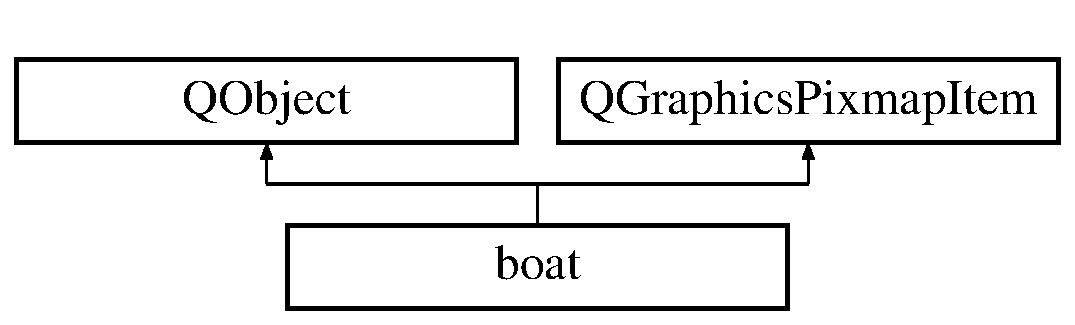
\includegraphics[height=2.000000cm]{classboat}
\end{center}
\end{figure}
\subsection*{Public Member Functions}
\begin{DoxyCompactItemize}
\item 
\hypertarget{classboat_a8cbefc8d0d8db323efcb8da6f05256f7}{\hyperlink{classboat_a8cbefc8d0d8db323efcb8da6f05256f7}{boat} (Q\-Object $\ast$parent=nullptr)}\label{classboat_a8cbefc8d0d8db323efcb8da6f05256f7}

\begin{DoxyCompactList}\small\item\em Setting \hyperlink{classPopeye}{Popeye}'s Image. \end{DoxyCompactList}\end{DoxyCompactItemize}


The documentation for this class was generated from the following files\-:\begin{DoxyCompactItemize}
\item 
\hyperlink{boat_8h}{boat.\-h}\item 
\hyperlink{boat_8cpp}{boat.\-cpp}\end{DoxyCompactItemize}

\hypertarget{classBug}{\section{Bug Class Reference}
\label{classBug}\index{Bug@{Bug}}
}
Inheritance diagram for Bug\-:\begin{figure}[H]
\begin{center}
\leavevmode
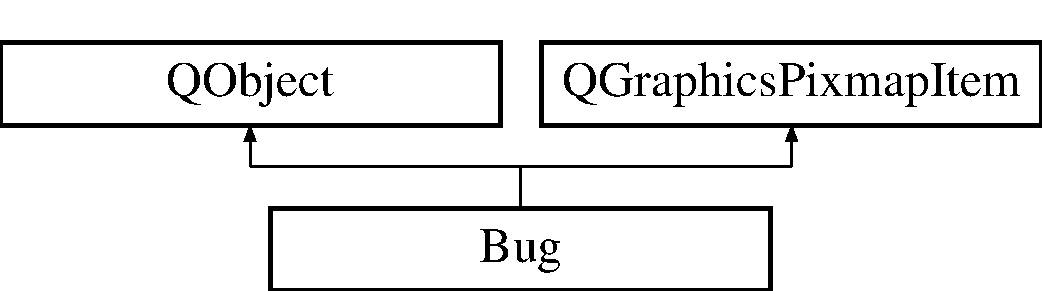
\includegraphics[height=2.000000cm]{classBug}
\end{center}
\end{figure}
\subsection*{Public Slots}
\begin{DoxyCompactItemize}
\item 
\hypertarget{classBug_ad968d4bb17f160ad412da3fa15d5417e}{void \hyperlink{classBug_ad968d4bb17f160ad412da3fa15d5417e}{guard} ()}\label{classBug_ad968d4bb17f160ad412da3fa15d5417e}

\begin{DoxyCompactList}\small\item\em The slot that moves the bug on each timer timeout. \end{DoxyCompactList}\item 
\hypertarget{classBug_ab1d53f066f74c84663c47028c1fdbe77}{void \hyperlink{classBug_ab1d53f066f74c84663c47028c1fdbe77}{shoot} ()}\label{classBug_ab1d53f066f74c84663c47028c1fdbe77}

\begin{DoxyCompactList}\small\item\em Responsible for the shooting logic of the \hyperlink{classBug}{Bug}. \end{DoxyCompactList}\end{DoxyCompactItemize}
\subsection*{Public Member Functions}
\begin{DoxyCompactItemize}
\item 
\hypertarget{classBug_ab8661834cbf8ea0d59bfcce05f8c19ac}{\hyperlink{classBug_ab8661834cbf8ea0d59bfcce05f8c19ac}{Bug} (\hyperlink{classGame2Scene}{Game2\-Scene} $\ast$)}\label{classBug_ab8661834cbf8ea0d59bfcce05f8c19ac}

\begin{DoxyCompactList}\small\item\em \hyperlink{classBug}{Bug} constructor. \end{DoxyCompactList}\item 
\hypertarget{classBug_a66fa2b39d8200535383e0feff494cd5c}{void \hyperlink{classBug_a66fa2b39d8200535383e0feff494cd5c}{decrement\-Lives} ()}\label{classBug_a66fa2b39d8200535383e0feff494cd5c}

\begin{DoxyCompactList}\small\item\em Responsible for collision logic with bullet. \end{DoxyCompactList}\item 
\hypertarget{classBug_ae009fdbc7055d30044e6b996fa89c6fc}{void \hyperlink{classBug_ae009fdbc7055d30044e6b996fa89c6fc}{pause} ()}\label{classBug_ae009fdbc7055d30044e6b996fa89c6fc}

\begin{DoxyCompactList}\small\item\em Responsible for keeping the bug in place when pausing the game. \end{DoxyCompactList}\item 
\hypertarget{classBug_ae634fa739fc20b7891fd0327fc78deae}{void \hyperlink{classBug_ae634fa739fc20b7891fd0327fc78deae}{resume} ()}\label{classBug_ae634fa739fc20b7891fd0327fc78deae}

\begin{DoxyCompactList}\small\item\em responsible for resuming after pausing \end{DoxyCompactList}\end{DoxyCompactItemize}
\subsection*{Public Attributes}
\begin{DoxyCompactItemize}
\item 
\hypertarget{classBug_af47aa4495bad729962a03d229d8fdb1c}{\hyperlink{classGame2Scene}{Game2\-Scene} $\ast$ \hyperlink{classBug_af47aa4495bad729962a03d229d8fdb1c}{scene}}\label{classBug_af47aa4495bad729962a03d229d8fdb1c}

\begin{DoxyCompactList}\small\item\em The scene where the bug is added. \end{DoxyCompactList}\item 
\hypertarget{classBug_aa75434e0a87bdefb7a80dbfa185b3cea}{Q\-Timer $\ast$ \hyperlink{classBug_aa75434e0a87bdefb7a80dbfa185b3cea}{timer}}\label{classBug_aa75434e0a87bdefb7a80dbfa185b3cea}

\begin{DoxyCompactList}\small\item\em Q\-Timer for moving the \hyperlink{classBug}{Bug} periodically. \end{DoxyCompactList}\item 
\hypertarget{classBug_a4fa5d0ebcd95fcd80a79f5b17c2d1c49}{Q\-Timer $\ast$ \hyperlink{classBug_a4fa5d0ebcd95fcd80a79f5b17c2d1c49}{shooting\-Timer}}\label{classBug_a4fa5d0ebcd95fcd80a79f5b17c2d1c49}

\begin{DoxyCompactList}\small\item\em Q\-Timer for shooting mini\-Bugs. \end{DoxyCompactList}\item 
\hypertarget{classBug_a31e919ead62893f77e673c6563a8fab2}{Q\-Pixmap $\ast$ \hyperlink{classBug_a31e919ead62893f77e673c6563a8fab2}{icon}}\label{classBug_a31e919ead62893f77e673c6563a8fab2}

\begin{DoxyCompactList}\small\item\em Q\-Pixmap holding the image of the \hyperlink{classBug}{Bug}. \end{DoxyCompactList}\item 
\hypertarget{classBug_a94745a4c20719851219de0fd11f699f4}{Q\-Transform {\bfseries transform}}\label{classBug_a94745a4c20719851219de0fd11f699f4}

\item 
\hypertarget{classBug_ac72cf078fdb04c5757417b7de8cbf64c}{int \hyperlink{classBug_ac72cf078fdb04c5757417b7de8cbf64c}{lives}}\label{classBug_ac72cf078fdb04c5757417b7de8cbf64c}

\begin{DoxyCompactList}\small\item\em Integer holding the number of \hyperlink{classBug}{Bug}'s lives left. \end{DoxyCompactList}\item 
\hypertarget{classBug_ace580e042da5ec607b1d6b2b06727185}{int \hyperlink{classBug_ace580e042da5ec607b1d6b2b06727185}{dir}}\label{classBug_ace580e042da5ec607b1d6b2b06727185}

\begin{DoxyCompactList}\small\item\em Integer holding the direction of movement of the \hyperlink{classBug}{Bug}. \end{DoxyCompactList}\item 
\hypertarget{classBug_af650f4d487abf1c9a2635a8348a69edc}{int {\bfseries i}}\label{classBug_af650f4d487abf1c9a2635a8348a69edc}

\end{DoxyCompactItemize}


The documentation for this class was generated from the following files\-:\begin{DoxyCompactItemize}
\item 
\hyperlink{bug_8h}{bug.\-h}\item 
\hyperlink{bug_8cpp}{bug.\-cpp}\end{DoxyCompactItemize}

\hypertarget{classBullet}{\section{Bullet Class Reference}
\label{classBullet}\index{Bullet@{Bullet}}
}
Inheritance diagram for Bullet\-:\begin{figure}[H]
\begin{center}
\leavevmode
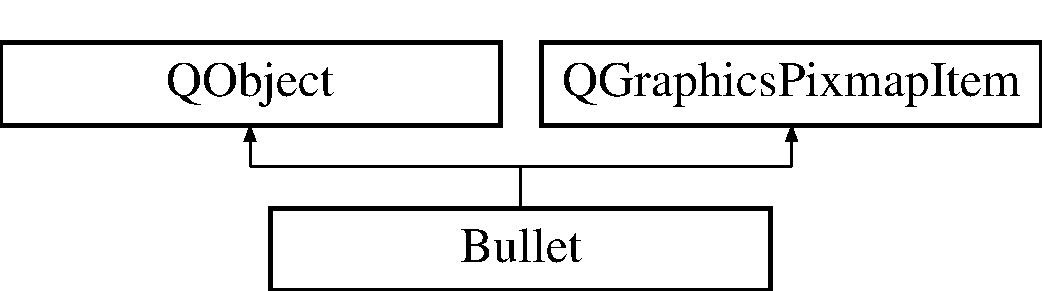
\includegraphics[height=2.000000cm]{classBullet}
\end{center}
\end{figure}
\subsection*{Public Slots}
\begin{DoxyCompactItemize}
\item 
\hypertarget{classBullet_a6140db968c42c05e829e142f74f20b16}{void \hyperlink{classBullet_a6140db968c42c05e829e142f74f20b16}{move} ()}\label{classBullet_a6140db968c42c05e829e142f74f20b16}

\begin{DoxyCompactList}\small\item\em The slot that moves the \hyperlink{classBullet}{Bullet} on the timer's timeout. \end{DoxyCompactList}\end{DoxyCompactItemize}
\subsection*{Public Member Functions}
\begin{DoxyCompactItemize}
\item 
\hypertarget{classBullet_a2c017a5fb7e34d169e26b2cfdd1bed28}{\hyperlink{classBullet_a2c017a5fb7e34d169e26b2cfdd1bed28}{Bullet} (int \hyperlink{classBullet_a368daaff6965adc373d8fec654e29ef0}{direction}, int x, int y, \hyperlink{classGame2Scene}{Game2\-Scene} $\ast$\hyperlink{classBullet_aeadd62cc1ee5aa7ce5fecdbe1f8685ed}{scene})}\label{classBullet_a2c017a5fb7e34d169e26b2cfdd1bed28}

\begin{DoxyCompactList}\small\item\em \hyperlink{classBullet}{Bullet} Constructor. \end{DoxyCompactList}\end{DoxyCompactItemize}
\subsection*{Public Attributes}
\begin{DoxyCompactItemize}
\item 
\hypertarget{classBullet_a48eb70e610461e300887a88aa8796ed4}{Q\-Pixmap $\ast$ \hyperlink{classBullet_a48eb70e610461e300887a88aa8796ed4}{icon}}\label{classBullet_a48eb70e610461e300887a88aa8796ed4}

\begin{DoxyCompactList}\small\item\em Q\-Pixmap holding the image of the bullet. \end{DoxyCompactList}\item 
\hypertarget{classBullet_a4958d1db2c416074d65eee3e3bc8fff5}{Q\-Timer $\ast$ \hyperlink{classBullet_a4958d1db2c416074d65eee3e3bc8fff5}{timer}}\label{classBullet_a4958d1db2c416074d65eee3e3bc8fff5}

\begin{DoxyCompactList}\small\item\em Q\-Timer that trigger s==s. \end{DoxyCompactList}\item 
\hypertarget{classBullet_aeadd62cc1ee5aa7ce5fecdbe1f8685ed}{\hyperlink{classGame2Scene}{Game2\-Scene} $\ast$ \hyperlink{classBullet_aeadd62cc1ee5aa7ce5fecdbe1f8685ed}{scene}}\label{classBullet_aeadd62cc1ee5aa7ce5fecdbe1f8685ed}

\begin{DoxyCompactList}\small\item\em The Scene where the \hyperlink{classBullet}{Bullet} is. \end{DoxyCompactList}\item 
\hypertarget{classBullet_a1a42b91927f84b3bb1170f3cd5855a14}{int \hyperlink{classBullet_a1a42b91927f84b3bb1170f3cd5855a14}{step}}\label{classBullet_a1a42b91927f84b3bb1170f3cd5855a14}

\begin{DoxyCompactList}\small\item\em A steps counter used for deleting the bullet at a certain range. \end{DoxyCompactList}\item 
\hypertarget{classBullet_a368daaff6965adc373d8fec654e29ef0}{int \hyperlink{classBullet_a368daaff6965adc373d8fec654e29ef0}{direction}}\label{classBullet_a368daaff6965adc373d8fec654e29ef0}

\begin{DoxyCompactList}\small\item\em Integer holding the direction of the \hyperlink{classBullet}{Bullet} according to the last step the tester made. \end{DoxyCompactList}\end{DoxyCompactItemize}


The documentation for this class was generated from the following files\-:\begin{DoxyCompactItemize}
\item 
\hyperlink{bullet_8h}{bullet.\-h}\item 
\hyperlink{bullet_8cpp}{bullet.\-cpp}\end{DoxyCompactItemize}

\hypertarget{classCoffeeCup}{\section{Coffee\-Cup Class Reference}
\label{classCoffeeCup}\index{Coffee\-Cup@{Coffee\-Cup}}
}
Inheritance diagram for Coffee\-Cup\-:\begin{figure}[H]
\begin{center}
\leavevmode
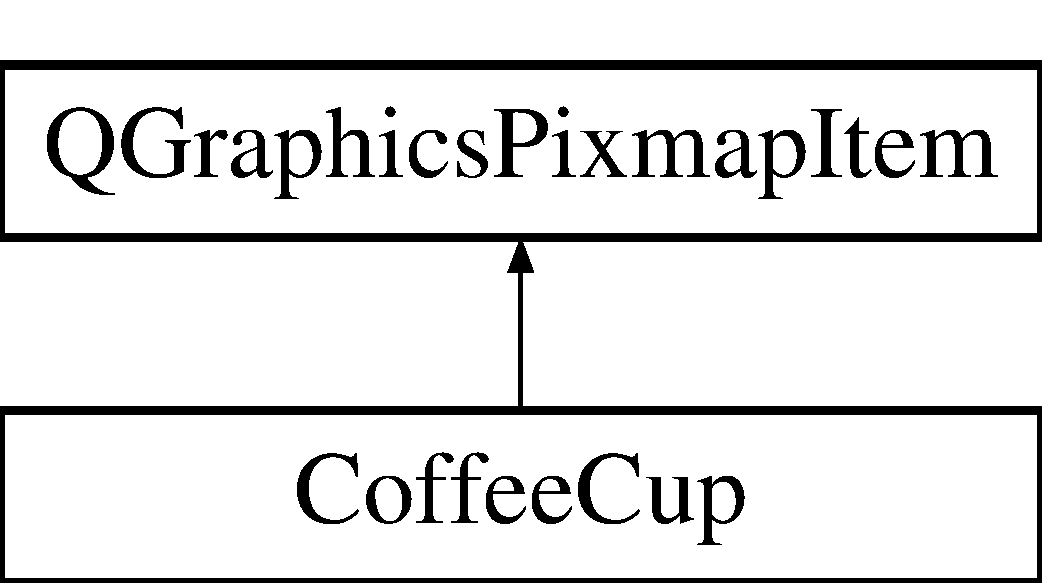
\includegraphics[height=2.000000cm]{classCoffeeCup}
\end{center}
\end{figure}
\subsection*{Public Member Functions}
\begin{DoxyCompactItemize}
\item 
\hypertarget{classCoffeeCup_aaf9cf1c1ed966a0027172dcc2ab07af2}{\hyperlink{classCoffeeCup_aaf9cf1c1ed966a0027172dcc2ab07af2}{Coffee\-Cup} ()}\label{classCoffeeCup_aaf9cf1c1ed966a0027172dcc2ab07af2}

\begin{DoxyCompactList}\small\item\em \hyperlink{classCoffeeCup}{Coffee\-Cup} Constructor. \end{DoxyCompactList}\end{DoxyCompactItemize}
\subsection*{Public Attributes}
\begin{DoxyCompactItemize}
\item 
\hypertarget{classCoffeeCup_a242ebac4b3a3a91bd4ee1fbe697e0c81}{Q\-Pixmap $\ast$ \hyperlink{classCoffeeCup_a242ebac4b3a3a91bd4ee1fbe697e0c81}{icon}}\label{classCoffeeCup_a242ebac4b3a3a91bd4ee1fbe697e0c81}

\begin{DoxyCompactList}\small\item\em Q\-Pixmap holding the image of the \hyperlink{classCoffeeCup}{Coffee\-Cup}. \end{DoxyCompactList}\end{DoxyCompactItemize}


The documentation for this class was generated from the following files\-:\begin{DoxyCompactItemize}
\item 
\hyperlink{coffeecup_8h}{coffeecup.\-h}\item 
\hyperlink{coffeecup_8cpp}{coffeecup.\-cpp}\end{DoxyCompactItemize}

\hypertarget{classgame1scene}{\section{game1scene Class Reference}
\label{classgame1scene}\index{game1scene@{game1scene}}
}
Inheritance diagram for game1scene\-:\begin{figure}[H]
\begin{center}
\leavevmode
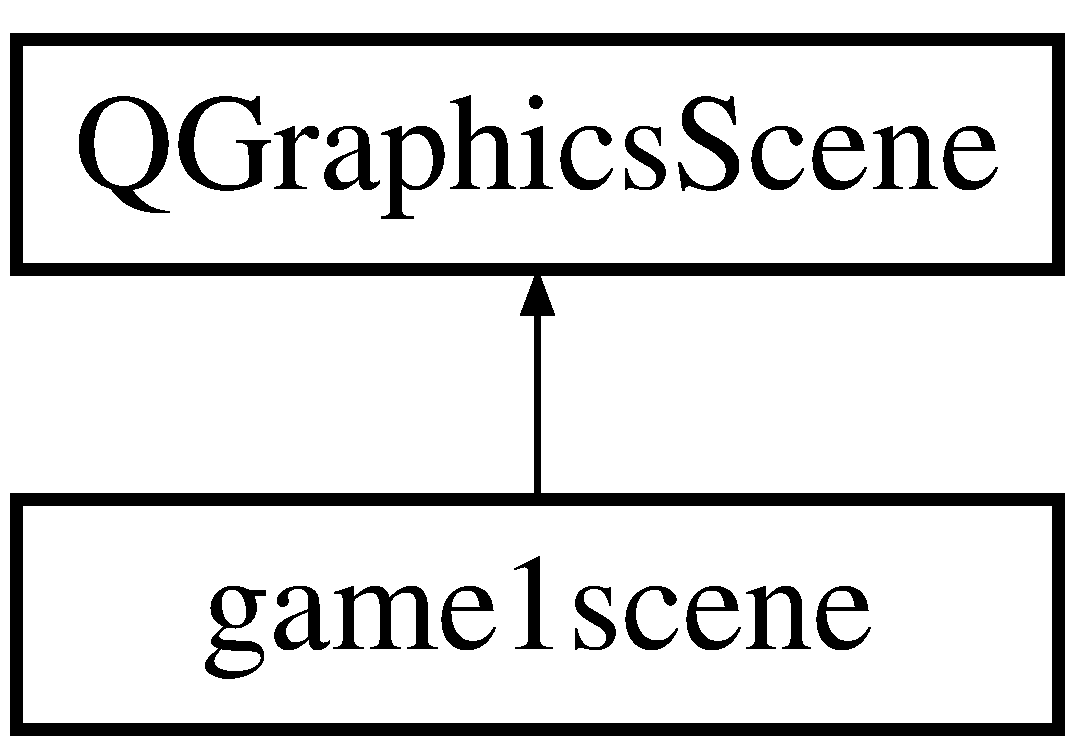
\includegraphics[height=2.000000cm]{classgame1scene}
\end{center}
\end{figure}
\subsection*{Public Slots}
\begin{DoxyCompactItemize}
\item 
void \hyperlink{classgame1scene_a2a94d8b07f6e0f122b59637f1dee8268}{start\-Level} ()
\begin{DoxyCompactList}\small\item\em start the appropriate level \end{DoxyCompactList}\item 
void \hyperlink{classgame1scene_a14c4c42a015d9fae66f80ca780794ee9}{update\-Countdown\-Timer} ()
\begin{DoxyCompactList}\small\item\em Function that will update the timer and then display it. \end{DoxyCompactList}\end{DoxyCompactItemize}
\subsection*{Public Member Functions}
\begin{DoxyCompactItemize}
\item 
\hyperlink{classgame1scene_af6cd7d94a19719f116b3afa5e49ee0ca}{game1scene} (Q\-String user)
\begin{DoxyCompactList}\small\item\em Default constructor. \end{DoxyCompactList}\item 
void \hyperlink{classgame1scene_a91bc63689e3a89ad7e854fd75434a453}{update\-Position1} ()
\begin{DoxyCompactList}\small\item\em update the position of popeye, placing him on top of the locks for level 1 \end{DoxyCompactList}\item 
void \hyperlink{classgame1scene_a442b205efa59a45cc3a7242e9536acb8}{update\-Position2} ()
\begin{DoxyCompactList}\small\item\em update the position of popeye, placing him on top of the locks for level 2 \end{DoxyCompactList}\item 
void \hyperlink{classgame1scene_ad05ad9fb2c1add7c2c5cfc3570451ebd}{update\-Position3} ()
\begin{DoxyCompactList}\small\item\em update the position of popeye, placing him on top of the locks for level 3 \end{DoxyCompactList}\item 
void \hyperlink{classgame1scene_a8ee0a0271db4868c6e1f5f74da26bf48}{update\-Position4} ()
\begin{DoxyCompactList}\small\item\em update the position of popeye, placing him on top of the locks for level 4 \end{DoxyCompactList}\item 
void \hyperlink{classgame1scene_aa970c577adf4b1c1a063224b2a837c3b}{update\-Position5} ()
\begin{DoxyCompactList}\small\item\em update the position of popeye, placing him on top of the locks for level 5 \end{DoxyCompactList}\item 
void \hyperlink{classgame1scene_a2b67ed62aefbb5e10754ba7657bff0d7}{update\-Position6} ()
\begin{DoxyCompactList}\small\item\em update the position of popeye, placing him on top of the locks for level 6 \end{DoxyCompactList}\item 
void \hyperlink{classgame1scene_a1adc8653395a15f6d294533f7a1c198f}{update\-Position7} ()
\begin{DoxyCompactList}\small\item\em update the position of popeye, placing him on top of the locks for level 7 \end{DoxyCompactList}\item 
void \hyperlink{classgame1scene_ae3e9b32b16773b3bc3e8629f4f83a767}{update\-Position8} ()
\begin{DoxyCompactList}\small\item\em update the position of popeye, placing him on top of the locks for level 8 \end{DoxyCompactList}\item 
\hypertarget{classgame1scene_aeda24597082614afc55ff852b2056234}{void \hyperlink{classgame1scene_aeda24597082614afc55ff852b2056234}{hide\-Level\-Scene} ()}\label{classgame1scene_aeda24597082614afc55ff852b2056234}

\begin{DoxyCompactList}\small\item\em update the position of popeye, placing him on top of the locks for level 1 \end{DoxyCompactList}\item 
int \hyperlink{classgame1scene_a924b36e709b2d27ca49eb80f9c006f0d}{get\-Level} ()
\begin{DoxyCompactList}\small\item\em get the user's level from the text file \end{DoxyCompactList}\item 
Q\-String\-List \hyperlink{classgame1scene_afbff10ae72de024ecdb698ede372fd1f}{profile\-Parser} (Q\-String line)
\begin{DoxyCompactList}\small\item\em get a list of string when parsing from text file the attributes that are seprated by spaces \end{DoxyCompactList}\item 
void \hyperlink{classgame1scene_a42ece47541b47ca9a82864785cddf84c}{set\-Up\-Countdown\-Timer} ()
\begin{DoxyCompactList}\small\item\em $<$ Timer controlling the countdown \end{DoxyCompactList}\end{DoxyCompactItemize}
\subsection*{Public Attributes}
\begin{DoxyCompactItemize}
\item 
\hypertarget{classgame1scene_ab1ace7e1dabcb9ddce4118018a4f302b}{\hyperlink{classPopeye}{Popeye} $\ast$ \hyperlink{classgame1scene_ab1ace7e1dabcb9ddce4118018a4f302b}{popeye} = new \hyperlink{classPopeye}{Popeye}()}\label{classgame1scene_ab1ace7e1dabcb9ddce4118018a4f302b}

\begin{DoxyCompactList}\small\item\em Creating the references to the Objects. \end{DoxyCompactList}\item 
\hypertarget{classgame1scene_a3fc55720e2521e19a949769d8f7a0ad7}{\hyperlink{classlocks}{locks} $\ast$ {\bfseries lock1} = new \hyperlink{classlocks}{locks}()}\label{classgame1scene_a3fc55720e2521e19a949769d8f7a0ad7}

\item 
\hypertarget{classgame1scene_a39bba452b809169bb94e57c761ff87b9}{\hyperlink{classlocks}{locks} $\ast$ {\bfseries lock2} = new \hyperlink{classlocks}{locks}()}\label{classgame1scene_a39bba452b809169bb94e57c761ff87b9}

\item 
\hypertarget{classgame1scene_a77d4f2e7cd11b5fbfb2d3ce801412010}{\hyperlink{classlocks}{locks} $\ast$ {\bfseries lock3} = new \hyperlink{classlocks}{locks}()}\label{classgame1scene_a77d4f2e7cd11b5fbfb2d3ce801412010}

\item 
\hypertarget{classgame1scene_a8da5c8b7cef2f68403d07c134b3da6ee}{\hyperlink{classlocks}{locks} $\ast$ {\bfseries lock4} = new \hyperlink{classlocks}{locks}()}\label{classgame1scene_a8da5c8b7cef2f68403d07c134b3da6ee}

\item 
\hypertarget{classgame1scene_ac63292ff2607add13a380b66abe46f50}{\hyperlink{classlocks}{locks} $\ast$ {\bfseries lock5} = new \hyperlink{classlocks}{locks}()}\label{classgame1scene_ac63292ff2607add13a380b66abe46f50}

\item 
\hypertarget{classgame1scene_ae0b1ea19ed5b5a95b19c7574bd134ca5}{\hyperlink{classlocks}{locks} $\ast$ {\bfseries lock6} = new \hyperlink{classlocks}{locks}()}\label{classgame1scene_ae0b1ea19ed5b5a95b19c7574bd134ca5}

\item 
\hypertarget{classgame1scene_a783433107de1418ee1ca5c82a2ba2155}{\hyperlink{classlocks}{locks} $\ast$ {\bfseries lock7} = new \hyperlink{classlocks}{locks}()}\label{classgame1scene_a783433107de1418ee1ca5c82a2ba2155}

\item 
\hypertarget{classgame1scene_a71c9197fc37bdbfa4c84a4896ff8fb1a}{\hyperlink{classlocks}{locks} $\ast$ {\bfseries lock8} = new \hyperlink{classlocks}{locks}()}\label{classgame1scene_a71c9197fc37bdbfa4c84a4896ff8fb1a}

\item 
\hypertarget{classgame1scene_a35dc8ff5e5eaf7fff1a49d192d67cf43}{Q\-Push\-Button $\ast$ {\bfseries start}}\label{classgame1scene_a35dc8ff5e5eaf7fff1a49d192d67cf43}

\item 
\hypertarget{classgame1scene_ac80d9732ed62e8a1453be6206e49b625}{Q\-String {\bfseries user}}\label{classgame1scene_ac80d9732ed62e8a1453be6206e49b625}

\item 
\hypertarget{classgame1scene_a117a936c1be44112e4c71a481121ecbb}{\hyperlink{classlevelsscene}{levelsscene} $\ast$ \hyperlink{classgame1scene_a117a936c1be44112e4c71a481121ecbb}{scene2}}\label{classgame1scene_a117a936c1be44112e4c71a481121ecbb}

\begin{DoxyCompactList}\small\item\em pointer to an Object of type levelsscene \end{DoxyCompactList}\item 
\hypertarget{classgame1scene_a5acd13b09ab8a8e73154e292633bbef3}{Q\-Graphics\-View $\ast$ \hyperlink{classgame1scene_a5acd13b09ab8a8e73154e292633bbef3}{view2}}\label{classgame1scene_a5acd13b09ab8a8e73154e292633bbef3}

\begin{DoxyCompactList}\small\item\em pointer to an Object of type Q\-Graphics\-View \end{DoxyCompactList}\item 
\hypertarget{classgame1scene_a9322202cbff7ba00ec16fa0163476238}{Q\-Graphics\-Text\-Item $\ast$ {\bfseries count\-Down\-Text}}\label{classgame1scene_a9322202cbff7ba00ec16fa0163476238}

\item 
\hypertarget{classgame1scene_abb3228cd05022e3f7ef04e3dee6d6910}{int {\bfseries countdown} = 12000}\label{classgame1scene_abb3228cd05022e3f7ef04e3dee6d6910}

\item 
\hypertarget{classgame1scene_ab149b18997176133c468be772976bec0}{Q\-Timer $\ast$ \hyperlink{classgame1scene_ab149b18997176133c468be772976bec0}{countdown\-Timer}}\label{classgame1scene_ab149b18997176133c468be772976bec0}

\begin{DoxyCompactList}\small\item\em $<$ value of the countdown at the start of the game that is = to 120 i.\-e. 20 mins to reach Olive \end{DoxyCompactList}\end{DoxyCompactItemize}


\subsection{Constructor \& Destructor Documentation}
\hypertarget{classgame1scene_af6cd7d94a19719f116b3afa5e49ee0ca}{\index{game1scene@{game1scene}!game1scene@{game1scene}}
\index{game1scene@{game1scene}!game1scene@{game1scene}}
\subsubsection[{game1scene}]{\setlength{\rightskip}{0pt plus 5cm}game1scene\-::game1scene (
\begin{DoxyParamCaption}
\item[{Q\-String}]{user}
\end{DoxyParamCaption}
)}}\label{classgame1scene_af6cd7d94a19719f116b3afa5e49ee0ca}


Default constructor. 

Setting the initial scene and object's positions. 

\subsection{Member Function Documentation}
\hypertarget{classgame1scene_a924b36e709b2d27ca49eb80f9c006f0d}{\index{game1scene@{game1scene}!get\-Level@{get\-Level}}
\index{get\-Level@{get\-Level}!game1scene@{game1scene}}
\subsubsection[{get\-Level}]{\setlength{\rightskip}{0pt plus 5cm}int game1scene\-::get\-Level (
\begin{DoxyParamCaption}
{}
\end{DoxyParamCaption}
)}}\label{classgame1scene_a924b36e709b2d27ca49eb80f9c006f0d}


get the user's level from the text file 

Getting the level number from the appropriate user text file (stored as the 10th entry)


\begin{DoxyParams}{Parameters}
{\em event} & only argument, key press \\
\hline
\end{DoxyParams}
\begin{DoxyReturn}{Returns}
int that is the Level Number 
\end{DoxyReturn}
$<$ to check if it is entering the file, and it is \hypertarget{classgame1scene_afbff10ae72de024ecdb698ede372fd1f}{\index{game1scene@{game1scene}!profile\-Parser@{profile\-Parser}}
\index{profile\-Parser@{profile\-Parser}!game1scene@{game1scene}}
\subsubsection[{profile\-Parser}]{\setlength{\rightskip}{0pt plus 5cm}Q\-String\-List game1scene\-::profile\-Parser (
\begin{DoxyParamCaption}
\item[{Q\-String}]{line}
\end{DoxyParamCaption}
)}}\label{classgame1scene_afbff10ae72de024ecdb698ede372fd1f}


get a list of string when parsing from text file the attributes that are seprated by spaces 

Parsing the text file that was filled and has his attributes seperated by tabs.

\begin{DoxyReturn}{Returns}
List of strings 
\end{DoxyReturn}
\hypertarget{classgame1scene_a42ece47541b47ca9a82864785cddf84c}{\index{game1scene@{game1scene}!set\-Up\-Countdown\-Timer@{set\-Up\-Countdown\-Timer}}
\index{set\-Up\-Countdown\-Timer@{set\-Up\-Countdown\-Timer}!game1scene@{game1scene}}
\subsubsection[{set\-Up\-Countdown\-Timer}]{\setlength{\rightskip}{0pt plus 5cm}void game1scene\-::set\-Up\-Countdown\-Timer (
\begin{DoxyParamCaption}
{}
\end{DoxyParamCaption}
)}}\label{classgame1scene_a42ece47541b47ca9a82864785cddf84c}


$<$ Timer controlling the countdown 

Initializes Text\-Item that indicates the Countdown at the start of each level.

Setting up the timer \hypertarget{classgame1scene_a2a94d8b07f6e0f122b59637f1dee8268}{\index{game1scene@{game1scene}!start\-Level@{start\-Level}}
\index{start\-Level@{start\-Level}!game1scene@{game1scene}}
\subsubsection[{start\-Level}]{\setlength{\rightskip}{0pt plus 5cm}void game1scene\-::start\-Level (
\begin{DoxyParamCaption}
{}
\end{DoxyParamCaption}
)\hspace{0.3cm}{\ttfamily [slot]}}}\label{classgame1scene_a2a94d8b07f6e0f122b59637f1dee8268}


start the appropriate level 

Starting the corresponsding level by calling the levelsscene constructure and updating the lock's positions accordingly. $<$ pointer to an Object of type levelsscene

$<$ pointer to an Object of type Q\-Graphics\-View \hypertarget{classgame1scene_a14c4c42a015d9fae66f80ca780794ee9}{\index{game1scene@{game1scene}!update\-Countdown\-Timer@{update\-Countdown\-Timer}}
\index{update\-Countdown\-Timer@{update\-Countdown\-Timer}!game1scene@{game1scene}}
\subsubsection[{update\-Countdown\-Timer}]{\setlength{\rightskip}{0pt plus 5cm}void game1scene\-::update\-Countdown\-Timer (
\begin{DoxyParamCaption}
{}
\end{DoxyParamCaption}
)\hspace{0.3cm}{\ttfamily [slot]}}}\label{classgame1scene_a14c4c42a015d9fae66f80ca780794ee9}


Function that will update the timer and then display it. 

update S\-L\-O\-T that controls the Countdown to display it when adjusted, every second \hypertarget{classgame1scene_a91bc63689e3a89ad7e854fd75434a453}{\index{game1scene@{game1scene}!update\-Position1@{update\-Position1}}
\index{update\-Position1@{update\-Position1}!game1scene@{game1scene}}
\subsubsection[{update\-Position1}]{\setlength{\rightskip}{0pt plus 5cm}void game1scene\-::update\-Position1 (
\begin{DoxyParamCaption}
{}
\end{DoxyParamCaption}
)}}\label{classgame1scene_a91bc63689e3a89ad7e854fd75434a453}


update the position of popeye, placing him on top of the locks for level 1 

Function Updating \hyperlink{classPopeye}{Popeye}'s position and hidding locks, according to the level Users' in. \hypertarget{classgame1scene_a442b205efa59a45cc3a7242e9536acb8}{\index{game1scene@{game1scene}!update\-Position2@{update\-Position2}}
\index{update\-Position2@{update\-Position2}!game1scene@{game1scene}}
\subsubsection[{update\-Position2}]{\setlength{\rightskip}{0pt plus 5cm}void game1scene\-::update\-Position2 (
\begin{DoxyParamCaption}
{}
\end{DoxyParamCaption}
)}}\label{classgame1scene_a442b205efa59a45cc3a7242e9536acb8}


update the position of popeye, placing him on top of the locks for level 2 

Function Updating \hyperlink{classPopeye}{Popeye}'s position and hidding locks, according to the level Users' in. \hypertarget{classgame1scene_ad05ad9fb2c1add7c2c5cfc3570451ebd}{\index{game1scene@{game1scene}!update\-Position3@{update\-Position3}}
\index{update\-Position3@{update\-Position3}!game1scene@{game1scene}}
\subsubsection[{update\-Position3}]{\setlength{\rightskip}{0pt plus 5cm}void game1scene\-::update\-Position3 (
\begin{DoxyParamCaption}
{}
\end{DoxyParamCaption}
)}}\label{classgame1scene_ad05ad9fb2c1add7c2c5cfc3570451ebd}


update the position of popeye, placing him on top of the locks for level 3 

Function Updating \hyperlink{classPopeye}{Popeye}'s position and hidding locks, according to the level Users' in. \hypertarget{classgame1scene_a8ee0a0271db4868c6e1f5f74da26bf48}{\index{game1scene@{game1scene}!update\-Position4@{update\-Position4}}
\index{update\-Position4@{update\-Position4}!game1scene@{game1scene}}
\subsubsection[{update\-Position4}]{\setlength{\rightskip}{0pt plus 5cm}void game1scene\-::update\-Position4 (
\begin{DoxyParamCaption}
{}
\end{DoxyParamCaption}
)}}\label{classgame1scene_a8ee0a0271db4868c6e1f5f74da26bf48}


update the position of popeye, placing him on top of the locks for level 4 

Function Updating \hyperlink{classPopeye}{Popeye}'s position and hidding locks, according to the level Users' in. \hypertarget{classgame1scene_aa970c577adf4b1c1a063224b2a837c3b}{\index{game1scene@{game1scene}!update\-Position5@{update\-Position5}}
\index{update\-Position5@{update\-Position5}!game1scene@{game1scene}}
\subsubsection[{update\-Position5}]{\setlength{\rightskip}{0pt plus 5cm}void game1scene\-::update\-Position5 (
\begin{DoxyParamCaption}
{}
\end{DoxyParamCaption}
)}}\label{classgame1scene_aa970c577adf4b1c1a063224b2a837c3b}


update the position of popeye, placing him on top of the locks for level 5 

Function Updating \hyperlink{classPopeye}{Popeye}'s position and hidding locks, according to the level Users' in. \hypertarget{classgame1scene_a2b67ed62aefbb5e10754ba7657bff0d7}{\index{game1scene@{game1scene}!update\-Position6@{update\-Position6}}
\index{update\-Position6@{update\-Position6}!game1scene@{game1scene}}
\subsubsection[{update\-Position6}]{\setlength{\rightskip}{0pt plus 5cm}void game1scene\-::update\-Position6 (
\begin{DoxyParamCaption}
{}
\end{DoxyParamCaption}
)}}\label{classgame1scene_a2b67ed62aefbb5e10754ba7657bff0d7}


update the position of popeye, placing him on top of the locks for level 6 

Function Updating \hyperlink{classPopeye}{Popeye}'s position and hidding locks, according to the level Users' in. \hypertarget{classgame1scene_a1adc8653395a15f6d294533f7a1c198f}{\index{game1scene@{game1scene}!update\-Position7@{update\-Position7}}
\index{update\-Position7@{update\-Position7}!game1scene@{game1scene}}
\subsubsection[{update\-Position7}]{\setlength{\rightskip}{0pt plus 5cm}void game1scene\-::update\-Position7 (
\begin{DoxyParamCaption}
{}
\end{DoxyParamCaption}
)}}\label{classgame1scene_a1adc8653395a15f6d294533f7a1c198f}


update the position of popeye, placing him on top of the locks for level 7 

Function Updating \hyperlink{classPopeye}{Popeye}'s position and hidding locks, according to the level Users' in. \hypertarget{classgame1scene_ae3e9b32b16773b3bc3e8629f4f83a767}{\index{game1scene@{game1scene}!update\-Position8@{update\-Position8}}
\index{update\-Position8@{update\-Position8}!game1scene@{game1scene}}
\subsubsection[{update\-Position8}]{\setlength{\rightskip}{0pt plus 5cm}void game1scene\-::update\-Position8 (
\begin{DoxyParamCaption}
{}
\end{DoxyParamCaption}
)}}\label{classgame1scene_ae3e9b32b16773b3bc3e8629f4f83a767}


update the position of popeye, placing him on top of the locks for level 8 

Function Updating \hyperlink{classPopeye}{Popeye}'s position and hidding locks, according to the level Users' in. 

The documentation for this class was generated from the following files\-:\begin{DoxyCompactItemize}
\item 
\hyperlink{game1scene_8h}{game1scene.\-h}\item 
\hyperlink{game1scene_8cpp}{game1scene.\-cpp}\end{DoxyCompactItemize}

\hypertarget{classGame2Scene}{\section{Game2\-Scene Class Reference}
\label{classGame2Scene}\index{Game2\-Scene@{Game2\-Scene}}
}
Inheritance diagram for Game2\-Scene\-:\begin{figure}[H]
\begin{center}
\leavevmode
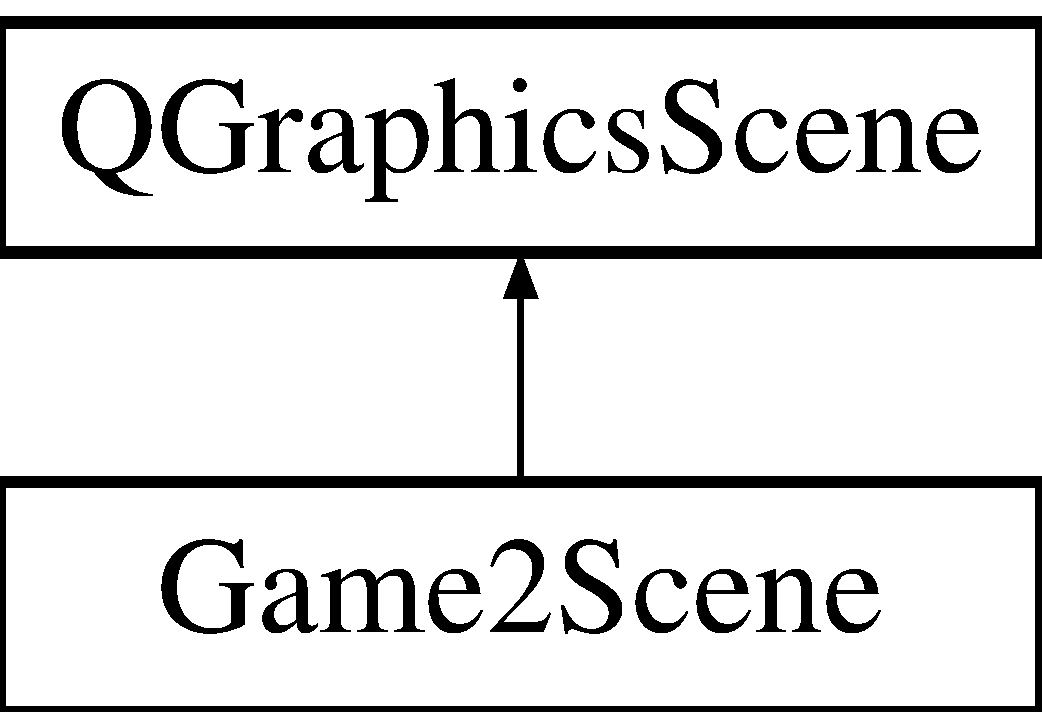
\includegraphics[height=2.000000cm]{classGame2Scene}
\end{center}
\end{figure}
\subsection*{Public Slots}
\begin{DoxyCompactItemize}
\item 
\hypertarget{classGame2Scene_aa54fef8cfc785656172fce2d4c035eec}{void \hyperlink{classGame2Scene_aa54fef8cfc785656172fce2d4c035eec}{deactivate\-Shield} ()}\label{classGame2Scene_aa54fef8cfc785656172fce2d4c035eec}

\begin{DoxyCompactList}\small\item\em Responsible of deactivating the shield on shield\-Timer timeout. \end{DoxyCompactList}\item 
\hypertarget{classGame2Scene_ac54e5865a35d342190b668418029255c}{void \hyperlink{classGame2Scene_ac54e5865a35d342190b668418029255c}{update\-Timer} ()}\label{classGame2Scene_ac54e5865a35d342190b668418029255c}

\begin{DoxyCompactList}\small\item\em Responsible of updating rem\-Sec on every timer timeout. \end{DoxyCompactList}\item 
\hypertarget{classGame2Scene_a0fce06771965e064807b71734effb3aa}{void \hyperlink{classGame2Scene_a0fce06771965e064807b71734effb3aa}{pause\-Or\-Resume} ()}\label{classGame2Scene_a0fce06771965e064807b71734effb3aa}

\begin{DoxyCompactList}\small\item\em Responsible of pausing or resuming the game on pause Push\-Button press. \end{DoxyCompactList}\item 
\hypertarget{classGame2Scene_ab26c015154dc7eaf33c3b1f009953492}{void \hyperlink{classGame2Scene_ab26c015154dc7eaf33c3b1f009953492}{start\-Level} ()}\label{classGame2Scene_ab26c015154dc7eaf33c3b1f009953492}

\begin{DoxyCompactList}\small\item\em Responsible of starting a new level after passing the previous one. \end{DoxyCompactList}\item 
\hypertarget{classGame2Scene_a70d447e24186449ec0a9fd67a42d0d1f}{void \hyperlink{classGame2Scene_a70d447e24186449ec0a9fd67a42d0d1f}{log\-Score} ()}\label{classGame2Scene_a70d447e24186449ec0a9fd67a42d0d1f}

\begin{DoxyCompactList}\small\item\em Responsible of logging the score to file after winning the game. \end{DoxyCompactList}\item 
\hypertarget{classGame2Scene_a7a63663bf7d3a79895bb56fe7240a9b2}{void \hyperlink{classGame2Scene_a7a63663bf7d3a79895bb56fe7240a9b2}{retry} ()}\label{classGame2Scene_a7a63663bf7d3a79895bb56fe7240a9b2}

\begin{DoxyCompactList}\small\item\em Responsible of restarting the game after losing. \end{DoxyCompactList}\end{DoxyCompactItemize}
\subsection*{Public Member Functions}
\begin{DoxyCompactItemize}
\item 
\hypertarget{classGame2Scene_a2bb661542400d8c3b9ac283c56ddec43}{\hyperlink{classGame2Scene_a2bb661542400d8c3b9ac283c56ddec43}{Game2\-Scene} (Q\-String \hyperlink{classGame2Scene_a03c78504fc8e5179a885307c8bf83c46}{user})}\label{classGame2Scene_a2bb661542400d8c3b9ac283c56ddec43}

\begin{DoxyCompactList}\small\item\em Constructor. \end{DoxyCompactList}\item 
\hypertarget{classGame2Scene_a316ab47115c7dfcd04d0374c7eff1195}{void \hyperlink{classGame2Scene_a316ab47115c7dfcd04d0374c7eff1195}{update\-Life\-Score} ()}\label{classGame2Scene_a316ab47115c7dfcd04d0374c7eff1195}

\begin{DoxyCompactList}\small\item\em Responsible of updating the tester's lives when colliding with a bug or a \hyperlink{classminiBug}{mini\-Bug}. \end{DoxyCompactList}\item 
int \hyperlink{classGame2Scene_aa2b1aab0dd957d2e5082d4c6352cf390}{get\-High\-Score} ()
\begin{DoxyCompactList}\small\item\em Responsible of fetching the High\-Score from the profile file. \end{DoxyCompactList}\item 
void \hyperlink{classGame2Scene_a8f2843e83fb8abbe454bf0ef0ef3c7ea}{update\-High\-Score} (Q\-String \hyperlink{classGame2Scene_a03c78504fc8e5179a885307c8bf83c46}{user})
\begin{DoxyCompactList}\small\item\em Responsible of updating the High\-Score in the profile file if needed. \end{DoxyCompactList}\end{DoxyCompactItemize}
\subsection*{Public Attributes}
\begin{DoxyCompactItemize}
\item 
\hypertarget{classGame2Scene_a8fd17e269efbee9884476ffef2c8d334}{int \hyperlink{classGame2Scene_a8fd17e269efbee9884476ffef2c8d334}{dir}}\label{classGame2Scene_a8fd17e269efbee9884476ffef2c8d334}

\begin{DoxyCompactList}\small\item\em Integer holding the direction of the tester. \end{DoxyCompactList}\item 
\hypertarget{classGame2Scene_a4e79ed93f76dbbdd93398f4095b1a656}{int \hyperlink{classGame2Scene_a4e79ed93f76dbbdd93398f4095b1a656}{ammo}}\label{classGame2Scene_a4e79ed93f76dbbdd93398f4095b1a656}

\begin{DoxyCompactList}\small\item\em Integer holding the amount of ammo left. \end{DoxyCompactList}\item 
\hypertarget{classGame2Scene_a6f7f39f987cfe21e8d75830dd017e64f}{int \hyperlink{classGame2Scene_a6f7f39f987cfe21e8d75830dd017e64f}{bugs}}\label{classGame2Scene_a6f7f39f987cfe21e8d75830dd017e64f}

\begin{DoxyCompactList}\small\item\em Integer holding the number of bugs left on the scene. \end{DoxyCompactList}\item 
\hypertarget{classGame2Scene_a9d666b1476d029c2db3d6361bef2b459}{int \hyperlink{classGame2Scene_a9d666b1476d029c2db3d6361bef2b459}{rem\-Sec}}\label{classGame2Scene_a9d666b1476d029c2db3d6361bef2b459}

\begin{DoxyCompactList}\small\item\em Integer holding the number of seconds left. \end{DoxyCompactList}\item 
\hypertarget{classGame2Scene_a298f56523cb98584b0bacc31bec34984}{int \hyperlink{classGame2Scene_a298f56523cb98584b0bacc31bec34984}{High\-Score}}\label{classGame2Scene_a298f56523cb98584b0bacc31bec34984}

\begin{DoxyCompactList}\small\item\em Integer holding the High\-Score of the Player. \end{DoxyCompactList}\item 
\hypertarget{classGame2Scene_a9a1966f21f97f746433e5425aa9b8ea3}{int \hyperlink{classGame2Scene_a9a1966f21f97f746433e5425aa9b8ea3}{score}}\label{classGame2Scene_a9a1966f21f97f746433e5425aa9b8ea3}

\begin{DoxyCompactList}\small\item\em Integer holding the current score of the player. \end{DoxyCompactList}\item 
\hypertarget{classGame2Scene_a49519fa674cd9c8ca8a9457417e85fc4}{int \hyperlink{classGame2Scene_a49519fa674cd9c8ca8a9457417e85fc4}{level}}\label{classGame2Scene_a49519fa674cd9c8ca8a9457417e85fc4}

\begin{DoxyCompactList}\small\item\em Integer holding the level the player is currently playing. \end{DoxyCompactList}\item 
\hypertarget{classGame2Scene_a6ff9cd19f3f72aed39ed8be062a29d7d}{bool \hyperlink{classGame2Scene_a6ff9cd19f3f72aed39ed8be062a29d7d}{playing}}\label{classGame2Scene_a6ff9cd19f3f72aed39ed8be062a29d7d}

\begin{DoxyCompactList}\small\item\em Boolean indicating if the player is active or not. \end{DoxyCompactList}\item 
\hypertarget{classGame2Scene_a9c1a6b684aef62653967b041bcf54d34}{bool \hyperlink{classGame2Scene_a9c1a6b684aef62653967b041bcf54d34}{has\-Shield}}\label{classGame2Scene_a9c1a6b684aef62653967b041bcf54d34}

\begin{DoxyCompactList}\small\item\em Boolean indicating if the tester has an active shiekd. \end{DoxyCompactList}\item 
\hypertarget{classGame2Scene_a05c4ee0ba558f497fb651df5ef5ce8ba}{bool \hyperlink{classGame2Scene_a05c4ee0ba558f497fb651df5ef5ce8ba}{Q\-Cshown}}\label{classGame2Scene_a05c4ee0ba558f497fb651df5ef5ce8ba}

\begin{DoxyCompactList}\small\item\em Boolean indicating if the Quality Control icon is hidden or shown. \end{DoxyCompactList}\item 
\hypertarget{classGame2Scene_a124c98a6c77d9fc892dda3b87bf9476f}{bool \hyperlink{classGame2Scene_a124c98a6c77d9fc892dda3b87bf9476f}{paused}}\label{classGame2Scene_a124c98a6c77d9fc892dda3b87bf9476f}

\begin{DoxyCompactList}\small\item\em Boolean indicating if the game is paused. \end{DoxyCompactList}\item 
\hypertarget{classGame2Scene_ac07f98d0be2ccfc03a6619ac0a8b124b}{Q\-List$<$ \hyperlink{classBug}{Bug} $\ast$ $>$ \hyperlink{classGame2Scene_ac07f98d0be2ccfc03a6619ac0a8b124b}{bug\-List}}\label{classGame2Scene_ac07f98d0be2ccfc03a6619ac0a8b124b}

\begin{DoxyCompactList}\small\item\em Q\-List of \hyperlink{classBug}{Bug} objects pointers. \end{DoxyCompactList}\item 
\hypertarget{classGame2Scene_a223238283a2e526ac893d96d40a676e9}{Q\-Label $\ast$ \hyperlink{classGame2Scene_a223238283a2e526ac893d96d40a676e9}{announcement}}\label{classGame2Scene_a223238283a2e526ac893d96d40a676e9}

\begin{DoxyCompactList}\small\item\em Q\-Label holding the win/loss announcements. \end{DoxyCompactList}\item 
\hypertarget{classGame2Scene_a345a19734cbec994392934782c7f570a}{Q\-Label $\ast$ \hyperlink{classGame2Scene_a345a19734cbec994392934782c7f570a}{timer\-Label}}\label{classGame2Scene_a345a19734cbec994392934782c7f570a}

\begin{DoxyCompactList}\small\item\em Q\-Label holding the string Timer. \end{DoxyCompactList}\item 
\hypertarget{classGame2Scene_ad6e653249d8185beff9c3ec0a065b22e}{Q\-Label $\ast$ \hyperlink{classGame2Scene_ad6e653249d8185beff9c3ec0a065b22e}{ammo\-Label}}\label{classGame2Scene_ad6e653249d8185beff9c3ec0a065b22e}

\begin{DoxyCompactList}\small\item\em Q\-Label holding the word Ammo. \end{DoxyCompactList}\item 
\hypertarget{classGame2Scene_ae17ea5202378d167508314349e97471d}{Q\-Label $\ast$ \hyperlink{classGame2Scene_ae17ea5202378d167508314349e97471d}{lives\-Label}}\label{classGame2Scene_ae17ea5202378d167508314349e97471d}

\begin{DoxyCompactList}\small\item\em Q\-Label holding the word Lives. \end{DoxyCompactList}\item 
\hypertarget{classGame2Scene_a7c2efee96429b9740203607dd7a40881}{Q\-Label $\ast$ {\bfseries Hi\-Score}}\label{classGame2Scene_a7c2efee96429b9740203607dd7a40881}

\item 
Q\-Label $\ast$ \hyperlink{classGame2Scene_ac135ec60d1ac545091a8a562df7e99cb}{score\-L}
\begin{DoxyCompactList}\small\item\em Q\-Label holding the word High\-Score. \end{DoxyCompactList}\item 
\hypertarget{classGame2Scene_aaa90ff637eec7f19523cf4debaed736d}{Q\-Push\-Button $\ast$ \hyperlink{classGame2Scene_aaa90ff637eec7f19523cf4debaed736d}{next}}\label{classGame2Scene_aaa90ff637eec7f19523cf4debaed736d}

\begin{DoxyCompactList}\small\item\em Q\-Push\-Button used to continue when level finishes;. \end{DoxyCompactList}\item 
\hypertarget{classGame2Scene_a08e755f5197834f770f07e86c6b5bbe4}{Q\-Push\-Button $\ast$ \hyperlink{classGame2Scene_a08e755f5197834f770f07e86c6b5bbe4}{pause}}\label{classGame2Scene_a08e755f5197834f770f07e86c6b5bbe4}

\begin{DoxyCompactList}\small\item\em Q\-Psuh\-Button used to pause/resume the. \end{DoxyCompactList}\item 
\hypertarget{classGame2Scene_a93036a156e84a8e5b56f0c66b634eed8}{\hyperlink{classLifeCounter}{Life\-Counter} $\ast$ \hyperlink{classGame2Scene_a93036a156e84a8e5b56f0c66b634eed8}{life\-Counter}}\label{classGame2Scene_a93036a156e84a8e5b56f0c66b634eed8}

\begin{DoxyCompactList}\small\item\em Q\-Graphics\-Pixmap\-Item representing the number of lives of the tester. \end{DoxyCompactList}\item 
\hypertarget{classGame2Scene_a8c8614db63839edac62c5bf35814a5c8}{\hyperlink{classLevelParser}{Level\-Parser} $\ast$ \hyperlink{classGame2Scene_a8c8614db63839edac62c5bf35814a5c8}{parser}}\label{classGame2Scene_a8c8614db63839edac62c5bf35814a5c8}

\begin{DoxyCompactList}\small\item\em Used to parse the levels from text files. \end{DoxyCompactList}\item 
\hypertarget{classGame2Scene_a03c78504fc8e5179a885307c8bf83c46}{Q\-String \hyperlink{classGame2Scene_a03c78504fc8e5179a885307c8bf83c46}{user}}\label{classGame2Scene_a03c78504fc8e5179a885307c8bf83c46}

\begin{DoxyCompactList}\small\item\em Q\-String holding the current user. \end{DoxyCompactList}\item 
\hypertarget{classGame2Scene_afb38ecf3a022b0f3f9102a507b4f60dd}{\hyperlink{classTester}{Tester} $\ast$ \hyperlink{classGame2Scene_afb38ecf3a022b0f3f9102a507b4f60dd}{tester}}\label{classGame2Scene_afb38ecf3a022b0f3f9102a507b4f60dd}

\begin{DoxyCompactList}\small\item\em Q\-Graphics\-Pixmap\-Item representing the tester character. \end{DoxyCompactList}\item 
\hypertarget{classGame2Scene_a176aa28a3941af04cb1f04b4a4d1f8c6}{\hyperlink{classQualityControlIcon}{Quality\-Control\-Icon} $\ast$ \hyperlink{classGame2Scene_a176aa28a3941af04cb1f04b4a4d1f8c6}{Q\-C\-Icon}}\label{classGame2Scene_a176aa28a3941af04cb1f04b4a4d1f8c6}

\begin{DoxyCompactList}\small\item\em Q\-Graphics\-Pixmap\-Item representing the Quality control Icon. \end{DoxyCompactList}\item 
\hypertarget{classGame2Scene_abd4d448b96cb584c41b5eb13ad7c100d}{Q\-Timer $\ast$ \hyperlink{classGame2Scene_abd4d448b96cb584c41b5eb13ad7c100d}{shield\-Timer}}\label{classGame2Scene_abd4d448b96cb584c41b5eb13ad7c100d}

\begin{DoxyCompactList}\small\item\em Q\-Timer responsible for deactivating the shield after 5 seconds. \end{DoxyCompactList}\item 
\hypertarget{classGame2Scene_a5a48dcdfc71f2f9cc3c7c37755b31b9e}{Q\-Timer $\ast$ \hyperlink{classGame2Scene_a5a48dcdfc71f2f9cc3c7c37755b31b9e}{timer}}\label{classGame2Scene_a5a48dcdfc71f2f9cc3c7c37755b31b9e}

\begin{DoxyCompactList}\small\item\em Q\-Timer responsible for updating the time each second. \end{DoxyCompactList}\item 
\hypertarget{classGame2Scene_a074f24b08fdd45db045bfd42a031a0bb}{Q\-Graphics\-Pixmap\-Item $\ast$ {\bfseries soul1}}\label{classGame2Scene_a074f24b08fdd45db045bfd42a031a0bb}

\item 
\hypertarget{classGame2Scene_a530af7b1147f2a7e960d62e086fa338c}{Q\-Graphics\-Pixmap\-Item $\ast$ {\bfseries soul2}}\label{classGame2Scene_a530af7b1147f2a7e960d62e086fa338c}

\item 
\hypertarget{classGame2Scene_addfdb5c43738ff25d5e4e385c8c1f18a}{Q\-Graphics\-Pixmap\-Item $\ast$ \hyperlink{classGame2Scene_addfdb5c43738ff25d5e4e385c8c1f18a}{soul3}}\label{classGame2Scene_addfdb5c43738ff25d5e4e385c8c1f18a}

\begin{DoxyCompactList}\small\item\em Q\-Graphics\-Pixmap\-Item representing the souls of the tester. \end{DoxyCompactList}\item 
\hypertarget{classGame2Scene_a2925920230b9269693709cd31e74beac}{Q\-Graphics\-Pixmap\-Item $\ast$ {\bfseries tens}}\label{classGame2Scene_a2925920230b9269693709cd31e74beac}

\item 
\hypertarget{classGame2Scene_af6b9f0c6a56d106c07a0d68ed3a7fb44}{Q\-Graphics\-Pixmap\-Item $\ast$ \hyperlink{classGame2Scene_af6b9f0c6a56d106c07a0d68ed3a7fb44}{units}}\label{classGame2Scene_af6b9f0c6a56d106c07a0d68ed3a7fb44}

\begin{DoxyCompactList}\small\item\em Q\-Graphics\-Pixmap\-Item representing the time left. \end{DoxyCompactList}\item 
\hypertarget{classGame2Scene_adcaf22f9ed4165aa5eb99eedb72445b5}{Q\-Graphics\-Pixmap\-Item $\ast$ {\bfseries ammo\-Tens}}\label{classGame2Scene_adcaf22f9ed4165aa5eb99eedb72445b5}

\item 
\hypertarget{classGame2Scene_a228893ef05a54bc3d67f4ec0b46d2198}{Q\-Graphics\-Pixmap\-Item $\ast$ \hyperlink{classGame2Scene_a228893ef05a54bc3d67f4ec0b46d2198}{ammo\-Units}}\label{classGame2Scene_a228893ef05a54bc3d67f4ec0b46d2198}

\begin{DoxyCompactList}\small\item\em Q\-Graphics\-Pixmap\-Item representing the ammo left. \end{DoxyCompactList}\end{DoxyCompactItemize}


\subsection{Member Function Documentation}
\hypertarget{classGame2Scene_aa2b1aab0dd957d2e5082d4c6352cf390}{\index{Game2\-Scene@{Game2\-Scene}!get\-High\-Score@{get\-High\-Score}}
\index{get\-High\-Score@{get\-High\-Score}!Game2Scene@{Game2\-Scene}}
\subsubsection[{get\-High\-Score}]{\setlength{\rightskip}{0pt plus 5cm}int Game2\-Scene\-::get\-High\-Score (
\begin{DoxyParamCaption}
{}
\end{DoxyParamCaption}
)}}\label{classGame2Scene_aa2b1aab0dd957d2e5082d4c6352cf390}


Responsible of fetching the High\-Score from the profile file. 

$<$ to check if it is entering the file, and it is \hypertarget{classGame2Scene_a8f2843e83fb8abbe454bf0ef0ef3c7ea}{\index{Game2\-Scene@{Game2\-Scene}!update\-High\-Score@{update\-High\-Score}}
\index{update\-High\-Score@{update\-High\-Score}!Game2Scene@{Game2\-Scene}}
\subsubsection[{update\-High\-Score}]{\setlength{\rightskip}{0pt plus 5cm}void Game2\-Scene\-::update\-High\-Score (
\begin{DoxyParamCaption}
\item[{Q\-String}]{user}
\end{DoxyParamCaption}
)}}\label{classGame2Scene_a8f2843e83fb8abbe454bf0ef0ef3c7ea}


Responsible of updating the High\-Score in the profile file if needed. 

$<$To update the level number in the text file (stored as the 10th entry) 

\subsection{Member Data Documentation}
\hypertarget{classGame2Scene_ac135ec60d1ac545091a8a562df7e99cb}{\index{Game2\-Scene@{Game2\-Scene}!score\-L@{score\-L}}
\index{score\-L@{score\-L}!Game2Scene@{Game2\-Scene}}
\subsubsection[{score\-L}]{\setlength{\rightskip}{0pt plus 5cm}Q\-Label$\ast$ Game2\-Scene\-::score\-L}}\label{classGame2Scene_ac135ec60d1ac545091a8a562df7e99cb}


Q\-Label holding the word High\-Score. 

Q\-Label holding the word score 

The documentation for this class was generated from the following files\-:\begin{DoxyCompactItemize}
\item 
\hyperlink{game2scene_8h}{game2scene.\-h}\item 
\hyperlink{game2scene_8cpp}{game2scene.\-cpp}\end{DoxyCompactItemize}

\hypertarget{classgameOver}{\section{game\-Over Class Reference}
\label{classgameOver}\index{game\-Over@{game\-Over}}
}
Inheritance diagram for game\-Over\-:\begin{figure}[H]
\begin{center}
\leavevmode
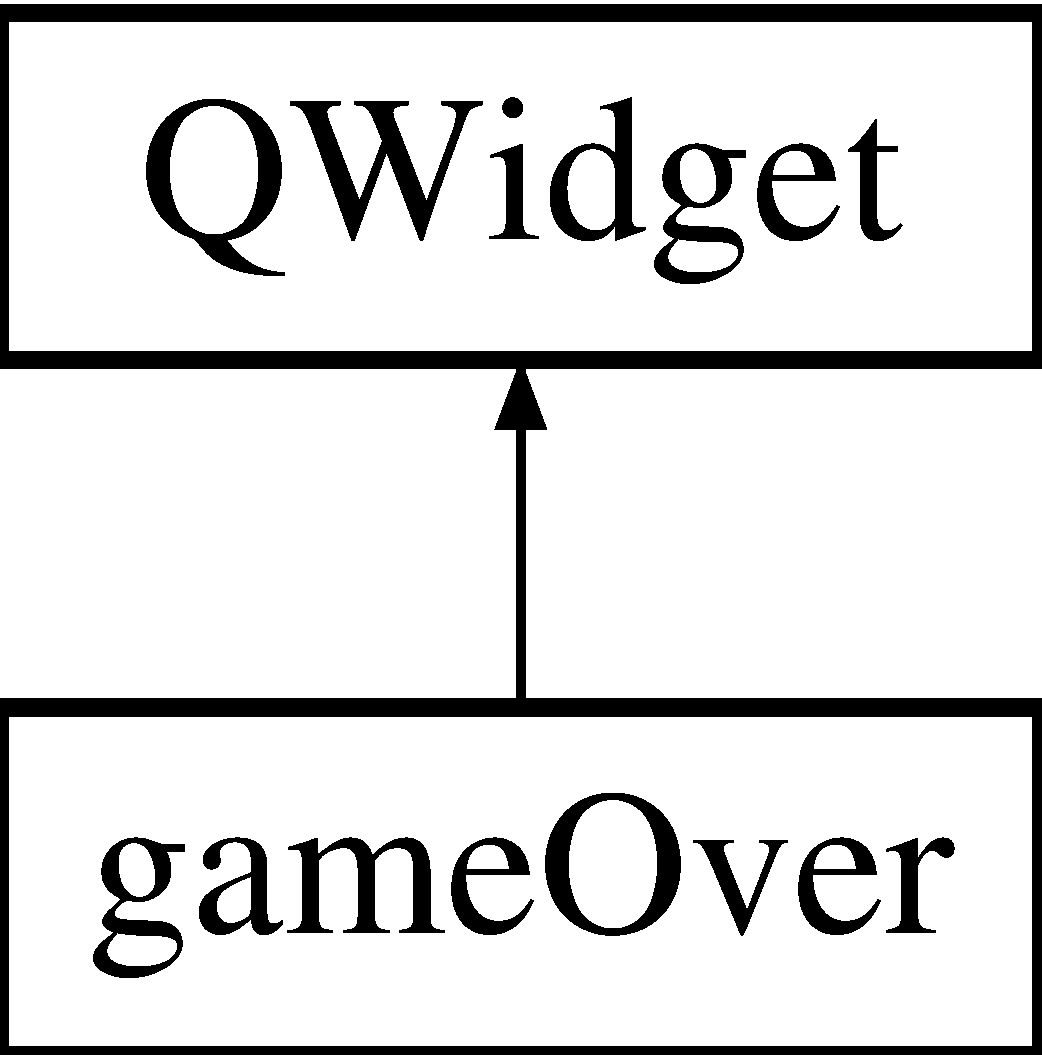
\includegraphics[height=2.000000cm]{classgameOver}
\end{center}
\end{figure}
\subsection*{Public Member Functions}
\begin{DoxyCompactItemize}
\item 
\hypertarget{classgameOver_a2aa791f3bc5d8899b4ee05210aafe69e}{\hyperlink{classgameOver_a2aa791f3bc5d8899b4ee05210aafe69e}{game\-Over} (Q\-Widget $\ast$parent=nullptr)}\label{classgameOver_a2aa791f3bc5d8899b4ee05210aafe69e}

\begin{DoxyCompactList}\small\item\em Setting the message pop up window content. \end{DoxyCompactList}\end{DoxyCompactItemize}


The documentation for this class was generated from the following files\-:\begin{DoxyCompactItemize}
\item 
gameover.\-h\item 
gameover.\-cpp\end{DoxyCompactItemize}

\hypertarget{classgamesWidget}{\section{games\-Widget Class Reference}
\label{classgamesWidget}\index{games\-Widget@{games\-Widget}}
}
Inheritance diagram for games\-Widget\-:\begin{figure}[H]
\begin{center}
\leavevmode
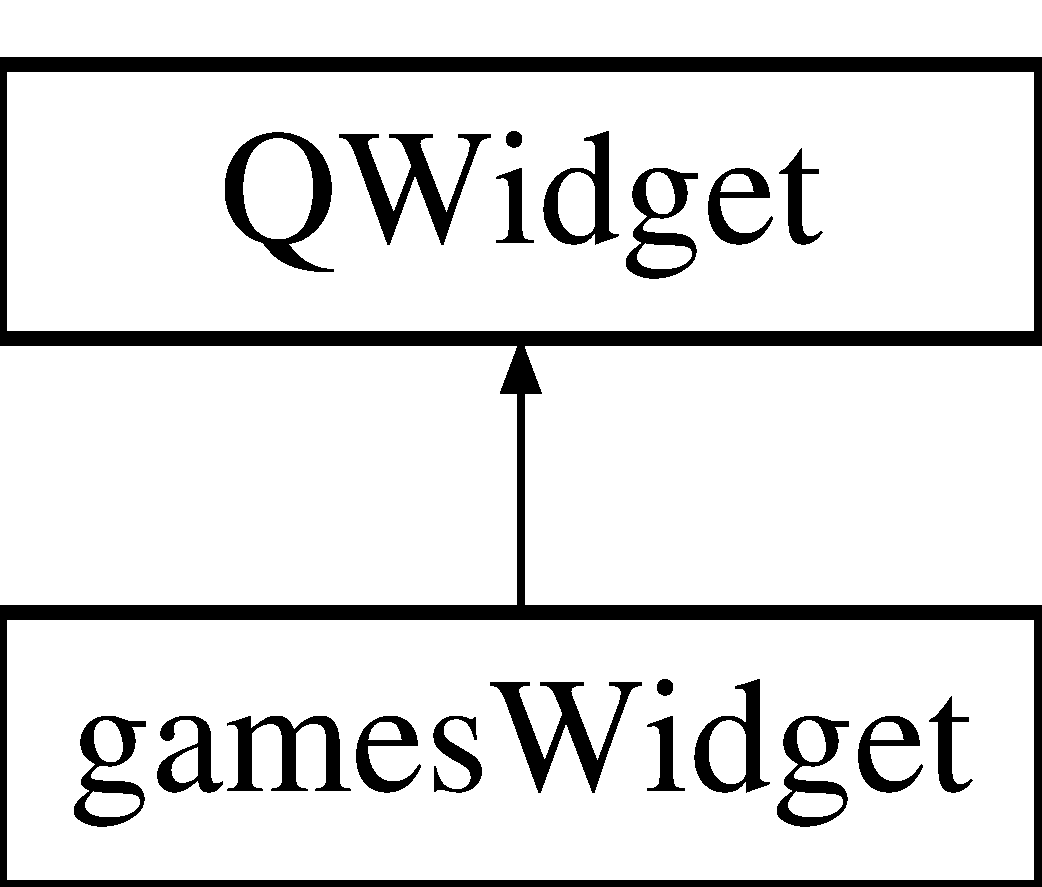
\includegraphics[height=2.000000cm]{classgamesWidget}
\end{center}
\end{figure}
\subsection*{Public Slots}
\begin{DoxyCompactItemize}
\item 
void \hyperlink{classgamesWidget_a746df5e5817b9c6bb1bc41dd97e0bd62}{start\-Game1} ()
\begin{DoxyCompactList}\small\item\em Slot to take the user to Game1\-Scene. \end{DoxyCompactList}\item 
\hypertarget{classgamesWidget_a6b9d62057de5bac6b65b4aa3a9dee61b}{void \hyperlink{classgamesWidget_a6b9d62057de5bac6b65b4aa3a9dee61b}{start\-Game2} ()}\label{classgamesWidget_a6b9d62057de5bac6b65b4aa3a9dee61b}

\begin{DoxyCompactList}\small\item\em Slot to take the user to \hyperlink{classGame2Scene}{Game2\-Scene}. \end{DoxyCompactList}\end{DoxyCompactItemize}
\subsection*{Public Member Functions}
\begin{DoxyCompactItemize}
\item 
\hypertarget{classgamesWidget_ac1a043599182281e3acd0f0d85a87139}{\hyperlink{classgamesWidget_ac1a043599182281e3acd0f0d85a87139}{games\-Widget} (Q\-String user)}\label{classgamesWidget_ac1a043599182281e3acd0f0d85a87139}

\begin{DoxyCompactList}\small\item\em Setting the widget's layout. \end{DoxyCompactList}\item 
\hypertarget{classgamesWidget_ae7a5777c497a04b964bd3d1acd0fa5b5}{void \hyperlink{classgamesWidget_ae7a5777c497a04b964bd3d1acd0fa5b5}{set\-Vertical\-Layout} ()}\label{classgamesWidget_ae7a5777c497a04b964bd3d1acd0fa5b5}

\begin{DoxyCompactList}\small\item\em Setting the Vertical Layout. \end{DoxyCompactList}\item 
\hypertarget{classgamesWidget_a1641bda0950365a1f6707fe56d08e004}{void \hyperlink{classgamesWidget_a1641bda0950365a1f6707fe56d08e004}{set\-Grid\-Layout} ()}\label{classgamesWidget_a1641bda0950365a1f6707fe56d08e004}

\begin{DoxyCompactList}\small\item\em Setting the Grid Layout. \end{DoxyCompactList}\end{DoxyCompactItemize}
\subsection*{Public Attributes}
\begin{DoxyCompactItemize}
\item 
\hypertarget{classgamesWidget_a96c63105c5ac277fc2549027d34624de}{Q\-Push\-Button $\ast$ {\bfseries game1}}\label{classgamesWidget_a96c63105c5ac277fc2549027d34624de}

\item 
\hypertarget{classgamesWidget_aebf0664e037955f85a1e46aa8d48ebd2}{Q\-Push\-Button $\ast$ {\bfseries game2}}\label{classgamesWidget_aebf0664e037955f85a1e46aa8d48ebd2}

\item 
\hypertarget{classgamesWidget_af077298d98486e4f58be7738d10ebd3c}{Q\-String {\bfseries user}}\label{classgamesWidget_af077298d98486e4f58be7738d10ebd3c}

\item 
\hypertarget{classgamesWidget_a68f0846d48f0c645eaa2dd1800405bd5}{Q\-V\-Box\-Layout $\ast$ {\bfseries Vertical\-L}}\label{classgamesWidget_a68f0846d48f0c645eaa2dd1800405bd5}

\item 
\hypertarget{classgamesWidget_ae91fa77d8e2d034136c58a1872b692e0}{Q\-Grid\-Layout $\ast$ {\bfseries Grid\-L}}\label{classgamesWidget_ae91fa77d8e2d034136c58a1872b692e0}

\item 
\hypertarget{classgamesWidget_a591d0422974904742d3c3d099e9e7439}{\hyperlink{classgame1scene}{game1scene} $\ast$ \hyperlink{classgamesWidget_a591d0422974904742d3c3d099e9e7439}{scene1}}\label{classgamesWidget_a591d0422974904742d3c3d099e9e7439}

\begin{DoxyCompactList}\small\item\em pointer to an Object of type \hyperlink{classgame1scene}{game1scene} \end{DoxyCompactList}\item 
\hypertarget{classgamesWidget_a376022b09f26245884e94e317b7cfed8}{\hyperlink{classGame2Scene}{Game2\-Scene} $\ast$ {\bfseries scene2}}\label{classgamesWidget_a376022b09f26245884e94e317b7cfed8}

\item 
\hypertarget{classgamesWidget_a273cf731a3523ad946313677890151a1}{Q\-Graphics\-View $\ast$ \hyperlink{classgamesWidget_a273cf731a3523ad946313677890151a1}{view1}}\label{classgamesWidget_a273cf731a3523ad946313677890151a1}

\begin{DoxyCompactList}\small\item\em pointer to an Object of type Q\-Graphics\-View \end{DoxyCompactList}\item 
\hypertarget{classgamesWidget_a431bcc98e9763d5fa02240e44e7e1844}{Q\-Graphics\-View $\ast$ {\bfseries view2}}\label{classgamesWidget_a431bcc98e9763d5fa02240e44e7e1844}

\end{DoxyCompactItemize}


\subsection{Member Function Documentation}
\hypertarget{classgamesWidget_a746df5e5817b9c6bb1bc41dd97e0bd62}{\index{games\-Widget@{games\-Widget}!start\-Game1@{start\-Game1}}
\index{start\-Game1@{start\-Game1}!gamesWidget@{games\-Widget}}
\subsubsection[{start\-Game1}]{\setlength{\rightskip}{0pt plus 5cm}void games\-Widget\-::start\-Game1 (
\begin{DoxyParamCaption}
{}
\end{DoxyParamCaption}
)\hspace{0.3cm}{\ttfamily [slot]}}}\label{classgamesWidget_a746df5e5817b9c6bb1bc41dd97e0bd62}


Slot to take the user to Game1\-Scene. 

$<$ pointer to an Object of type \hyperlink{classgame1scene}{game1scene}

$<$ pointer to an Object of type Q\-Graphics\-View 

The documentation for this class was generated from the following files\-:\begin{DoxyCompactItemize}
\item 
gameswidget.\-h\item 
\hyperlink{gameswidget_8cpp}{gameswidget.\-cpp}\end{DoxyCompactItemize}

\hypertarget{classhints}{\section{hints Class Reference}
\label{classhints}\index{hints@{hints}}
}
Inheritance diagram for hints\-:\begin{figure}[H]
\begin{center}
\leavevmode
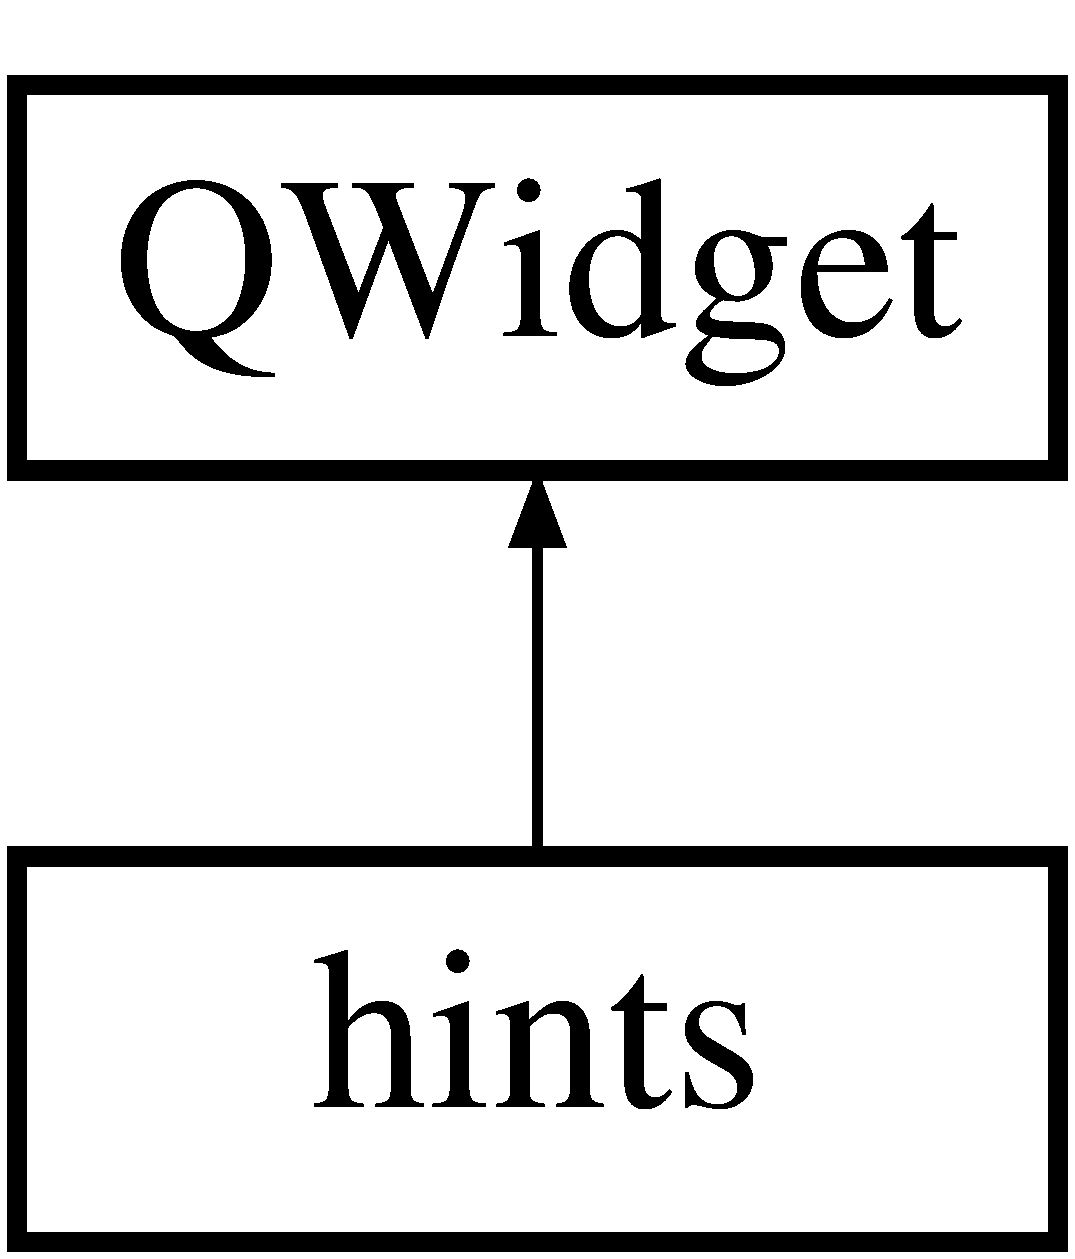
\includegraphics[height=2.000000cm]{classhints}
\end{center}
\end{figure}
\subsection*{Public Member Functions}
\begin{DoxyCompactItemize}
\item 
\hypertarget{classhints_a2d10c2dc601483be08f4ee46f1a6f209}{\hyperlink{classhints_a2d10c2dc601483be08f4ee46f1a6f209}{hints} (Q\-Widget $\ast$parent=nullptr)}\label{classhints_a2d10c2dc601483be08f4ee46f1a6f209}

\begin{DoxyCompactList}\small\item\em Setting the hints pop up window content. \end{DoxyCompactList}\item 
\hypertarget{classhints_aa0d8580e6afded471d91c78e9324c557}{{\bfseries hints} (Q\-String hint, Q\-Widget $\ast$parent=nullptr)}\label{classhints_aa0d8580e6afded471d91c78e9324c557}

\end{DoxyCompactItemize}


The documentation for this class was generated from the following files\-:\begin{DoxyCompactItemize}
\item 
\hyperlink{hints_8h}{hints.\-h}\item 
\hyperlink{hints_8cpp}{hints.\-cpp}\end{DoxyCompactItemize}

\hypertarget{classinstruction}{\section{instruction Class Reference}
\label{classinstruction}\index{instruction@{instruction}}
}
Inheritance diagram for instruction\-:\begin{figure}[H]
\begin{center}
\leavevmode
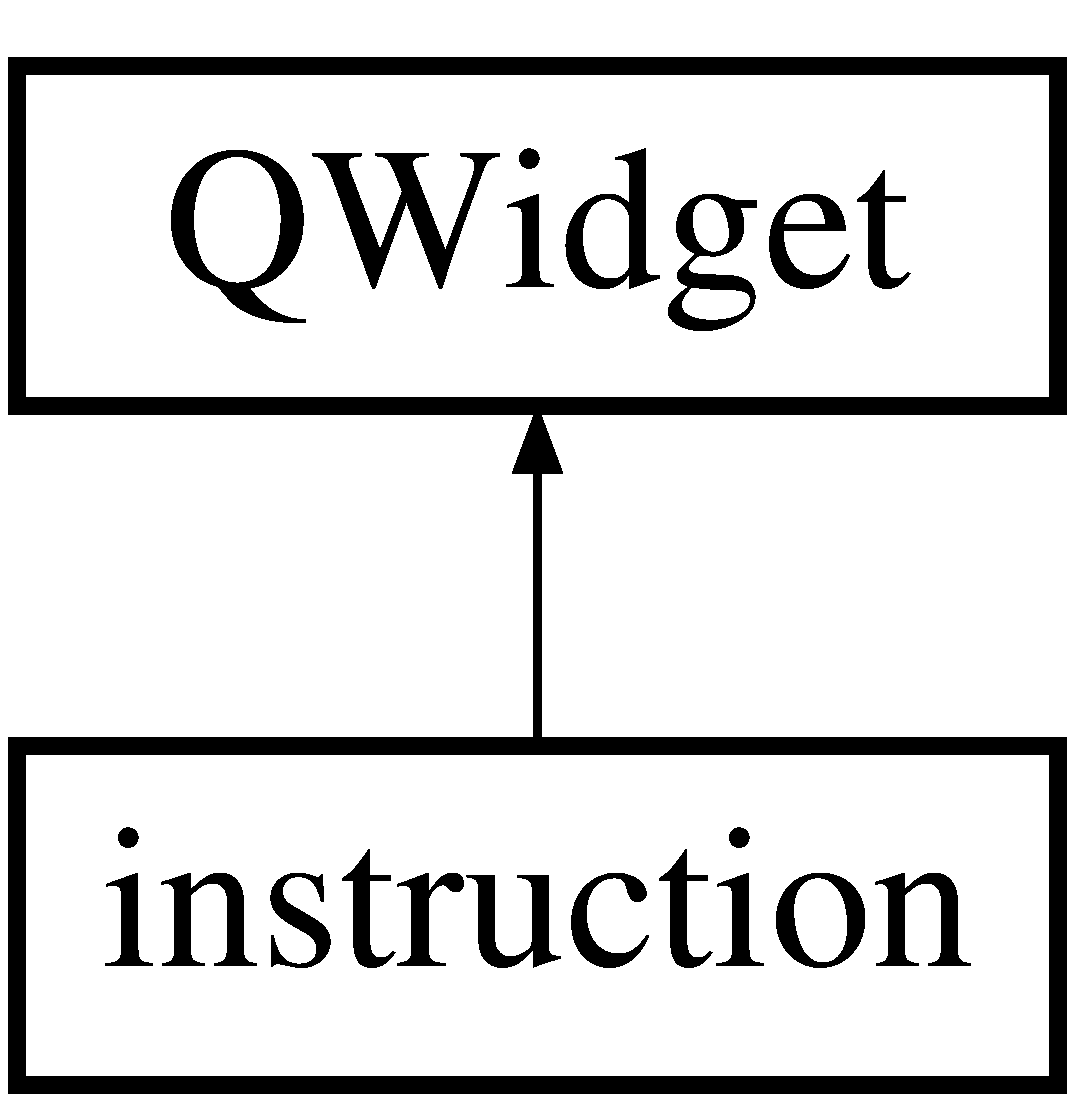
\includegraphics[height=2.000000cm]{classinstruction}
\end{center}
\end{figure}
\subsection*{Public Member Functions}
\begin{DoxyCompactItemize}
\item 
\hypertarget{classinstruction_a8d62f94c25b1e482cc5f71cdf593e70e}{\hyperlink{classinstruction_a8d62f94c25b1e482cc5f71cdf593e70e}{instruction} (Q\-Widget $\ast$parent=nullptr)}\label{classinstruction_a8d62f94c25b1e482cc5f71cdf593e70e}

\begin{DoxyCompactList}\small\item\em Setting the instruction pop up window content. \end{DoxyCompactList}\end{DoxyCompactItemize}


The documentation for this class was generated from the following files\-:\begin{DoxyCompactItemize}
\item 
\hyperlink{instruction_8h}{instruction.\-h}\item 
\hyperlink{instruction_8cpp}{instruction.\-cpp}\end{DoxyCompactItemize}

\hypertarget{classLevelParser}{\section{Level\-Parser Class Reference}
\label{classLevelParser}\index{Level\-Parser@{Level\-Parser}}
}
\subsection*{Public Member Functions}
\begin{DoxyCompactItemize}
\item 
\hypertarget{classLevelParser_aee5be22392eab36591fe956f4cf39baa}{\hyperlink{classLevelParser_aee5be22392eab36591fe956f4cf39baa}{Level\-Parser} (Q\-String \hyperlink{classLevelParser_a065b58408c0fef7d7d72930512fe069f}{file\-Path})}\label{classLevelParser_aee5be22392eab36591fe956f4cf39baa}

\begin{DoxyCompactList}\small\item\em Constructor. \end{DoxyCompactList}\item 
\hypertarget{classLevelParser_ab04f9b5381ec9ba9ab729a43b76e6284}{void \hyperlink{classLevelParser_ab04f9b5381ec9ba9ab729a43b76e6284}{parse} (\hyperlink{classGame2Scene}{Game2\-Scene} $\ast$scene)}\label{classLevelParser_ab04f9b5381ec9ba9ab729a43b76e6284}

\begin{DoxyCompactList}\small\item\em Responsible of actually parsing the file and adding the elements to the scene. \end{DoxyCompactList}\end{DoxyCompactItemize}
\subsection*{Public Attributes}
\begin{DoxyCompactItemize}
\item 
\hypertarget{classLevelParser_a065b58408c0fef7d7d72930512fe069f}{Q\-Dir $\ast$ \hyperlink{classLevelParser_a065b58408c0fef7d7d72930512fe069f}{file\-Path}}\label{classLevelParser_a065b58408c0fef7d7d72930512fe069f}

\begin{DoxyCompactList}\small\item\em Directory to the file being parsed. \end{DoxyCompactList}\end{DoxyCompactItemize}


The documentation for this class was generated from the following files\-:\begin{DoxyCompactItemize}
\item 
\hyperlink{levelparser_8h}{levelparser.\-h}\item 
\hyperlink{levelparser_8cpp}{levelparser.\-cpp}\end{DoxyCompactItemize}

\hypertarget{classlevels}{\section{levels Class Reference}
\label{classlevels}\index{levels@{levels}}
}
\subsection*{Public Member Functions}
\begin{DoxyCompactItemize}
\item 
\hypertarget{classlevels_a9e8ec5991208108571714afff927eb6d}{\hyperlink{classlevels_a9e8ec5991208108571714afff927eb6d}{levels} (int x, Q\-String user)}\label{classlevels_a9e8ec5991208108571714afff927eb6d}

\begin{DoxyCompactList}\small\item\em Setting the specs for each level. \end{DoxyCompactList}\item 
void \hyperlink{classlevels_a7034ce39cdf8b339af99155ea4950152}{set\-Popeye\-X1} (int new\-X)
\begin{DoxyCompactList}\small\item\em Setting up popeye's X and Y positions. \end{DoxyCompactList}\item 
\hypertarget{classlevels_af6ee2e921b62c41227a4e6c602bb9305}{void \hyperlink{classlevels_af6ee2e921b62c41227a4e6c602bb9305}{set\-Popeye\-Y1} (int new\-Y)}\label{classlevels_af6ee2e921b62c41227a4e6c602bb9305}

\begin{DoxyCompactList}\small\item\em Setting \hyperlink{classPopeye}{Popeye}'s New Y position. \end{DoxyCompactList}\item 
void \hyperlink{classlevels_a1591c1aaea4c1c22bf7ef9641882e47c}{increment\-Hint\-Number} ()
\begin{DoxyCompactList}\small\item\em Incrementing the hint Number. \end{DoxyCompactList}\item 
void \hyperlink{classlevels_a676d095442c1da53bbf6dbb99c7509ae}{reset\-Hint\-Number} ()
\begin{DoxyCompactList}\small\item\em Restting the hint Number. \end{DoxyCompactList}\item 
\hypertarget{classlevels_af7799e2944f4f3cf30915976ca2ebe81}{void \hyperlink{classlevels_af7799e2944f4f3cf30915976ca2ebe81}{decrement\-Lifes} ()}\label{classlevels_af7799e2944f4f3cf30915976ca2ebe81}

\begin{DoxyCompactList}\small\item\em Decrementing the number of lifes. \end{DoxyCompactList}\item 
\hypertarget{classlevels_aa11fc016871dae129e82668fc96a2494}{void \hyperlink{classlevels_aa11fc016871dae129e82668fc96a2494}{increment\-Level\-Numb} ()}\label{classlevels_aa11fc016871dae129e82668fc96a2494}

\begin{DoxyCompactList}\small\item\em Incrementing the Level Number. \end{DoxyCompactList}\item 
\hypertarget{classlevels_a7e6afe3cac1e779d5853f8dba7b4e5fc}{void \hyperlink{classlevels_a7e6afe3cac1e779d5853f8dba7b4e5fc}{increment\-Score} ()}\label{classlevels_a7e6afe3cac1e779d5853f8dba7b4e5fc}

\begin{DoxyCompactList}\small\item\em Incrementing the score. \end{DoxyCompactList}\item 
\hypertarget{classlevels_a0a822208ede36535819614b9567f514d}{void \hyperlink{classlevels_a0a822208ede36535819614b9567f514d}{decrement\-Score} ()}\label{classlevels_a0a822208ede36535819614b9567f514d}

\begin{DoxyCompactList}\small\item\em Decrementing the score. \end{DoxyCompactList}\item 
void \hyperlink{classlevels_a34d3e8e41addbd72aa48e1a9000f8fdd}{update\-Level} (Q\-String user)
\begin{DoxyCompactList}\small\item\em Updating the level Number when user passes a level. \end{DoxyCompactList}\item 
void \hyperlink{classlevels_ac87ef97458bf84ba939ec0e06833a0fc}{update\-Level\-One} (Q\-String user)
\begin{DoxyCompactList}\small\item\em Reseting the user's level to 1 if he looses the game. \end{DoxyCompactList}\item 
int \hyperlink{classlevels_afbaaf65ea0eec78856a2844a5f2effb6}{get\-Score} (Q\-String user)
\item 
void \hyperlink{classlevels_ad768338c2e60e0a55ad8655ae44e3d4f}{update\-Score} (Q\-String user)
\item 
void \hyperlink{classlevels_ab33b252392e1de5318895f306ff30be6}{reset\-Lives} ()
\begin{DoxyCompactList}\small\item\em Reseting the lifes to it's initial count of 5. \end{DoxyCompactList}\item 
\hypertarget{classlevels_a17d7e0f2c9a88471180b352bd7c7885e}{void \hyperlink{classlevels_a17d7e0f2c9a88471180b352bd7c7885e}{reset\-Score} ()}\label{classlevels_a17d7e0f2c9a88471180b352bd7c7885e}

\begin{DoxyCompactList}\small\item\em Reseting the score to it's initial count of 100. \end{DoxyCompactList}\item 
Q\-String\-List \hyperlink{classlevels_ac405da2d15ad7eb0db63b841ec243ad4}{profile\-Parser} (Q\-String)
\begin{DoxyCompactList}\small\item\em parse the line in a text file and return a list of strings \end{DoxyCompactList}\end{DoxyCompactItemize}
\subsection*{Public Attributes}
\begin{DoxyCompactItemize}
\item 
\hypertarget{classlevels_a6a07ae56f660f054725780f8c6c98d4a}{Q\-String {\bfseries hint} \mbox{[}3\mbox{]}}\label{classlevels_a6a07ae56f660f054725780f8c6c98d4a}

\item 
\hypertarget{classlevels_a0b030ae621e2134027a38ae9071be3d8}{Q\-String {\bfseries instructions}}\label{classlevels_a0b030ae621e2134027a38ae9071be3d8}

\item 
\hypertarget{classlevels_a2d25044468ead143b92458188a88720d}{int {\bfseries popeye\-X1}}\label{classlevels_a2d25044468ead143b92458188a88720d}

\item 
\hypertarget{classlevels_a7e5dd0abebbfe2a2f1706c1e1ff45d31}{int \hyperlink{classlevels_a7e5dd0abebbfe2a2f1706c1e1ff45d31}{popeye\-Y1}}\label{classlevels_a7e5dd0abebbfe2a2f1706c1e1ff45d31}

\begin{DoxyCompactList}\small\item\em popeye's X and Y positions \end{DoxyCompactList}\item 
\hypertarget{classlevels_a73c8cdfbef251072bf35c7722d478356}{int {\bfseries spinach\-X1}}\label{classlevels_a73c8cdfbef251072bf35c7722d478356}

\item 
\hypertarget{classlevels_aaae2e10293156b0bc6352cab3752e7f4}{int {\bfseries spinach\-Y1}}\label{classlevels_aaae2e10293156b0bc6352cab3752e7f4}

\item 
\hypertarget{classlevels_a1a9a5432ebebde76cae16a6c66c72ca4}{int {\bfseries spinach\-X2}}\label{classlevels_a1a9a5432ebebde76cae16a6c66c72ca4}

\item 
\hypertarget{classlevels_a5fdb199dd540d4c6ae719a3abbb0a3bf}{int {\bfseries spinach\-Y2}}\label{classlevels_a5fdb199dd540d4c6ae719a3abbb0a3bf}

\item 
\hypertarget{classlevels_a8930bfc6fc9cc515afe6a3cbb926a60a}{int {\bfseries spinach\-X3}}\label{classlevels_a8930bfc6fc9cc515afe6a3cbb926a60a}

\item 
\hypertarget{classlevels_a52e9e72bba3e0a66fdfccf7d30199b73}{int \hyperlink{classlevels_a52e9e72bba3e0a66fdfccf7d30199b73}{spinach\-Y3}}\label{classlevels_a52e9e72bba3e0a66fdfccf7d30199b73}

\begin{DoxyCompactList}\small\item\em spinach can's X and Y positions \end{DoxyCompactList}\item 
\hypertarget{classlevels_ac5ae82c88e0d7abd374474b4eefe9346}{int {\bfseries river1\-X}}\label{classlevels_ac5ae82c88e0d7abd374474b4eefe9346}

\item 
\hypertarget{classlevels_a3584b0cea2829a68285f3eca74380762}{int \hyperlink{classlevels_a3584b0cea2829a68285f3eca74380762}{river1\-Y}}\label{classlevels_a3584b0cea2829a68285f3eca74380762}

\begin{DoxyCompactList}\small\item\em the river's X and Y positions \end{DoxyCompactList}\item 
\hypertarget{classlevels_a6b56a9191845fd4d69f73c086564e638}{int {\bfseries boat1\-X}}\label{classlevels_a6b56a9191845fd4d69f73c086564e638}

\item 
\hypertarget{classlevels_a7b9433d0d89fc66d1edde51e37d0d22a}{int \hyperlink{classlevels_a7b9433d0d89fc66d1edde51e37d0d22a}{boat1\-Y}}\label{classlevels_a7b9433d0d89fc66d1edde51e37d0d22a}

\begin{DoxyCompactList}\small\item\em the boat's X and Y positions \end{DoxyCompactList}\item 
\hypertarget{classlevels_a0e02b45c06a5d80ad70dc093f2c4f060}{int {\bfseries rock1\-X}}\label{classlevels_a0e02b45c06a5d80ad70dc093f2c4f060}

\item 
\hypertarget{classlevels_a297c63c2b287658df28f941127c4ecda}{int \hyperlink{classlevels_a297c63c2b287658df28f941127c4ecda}{rock1\-Y}}\label{classlevels_a297c63c2b287658df28f941127c4ecda}

\begin{DoxyCompactList}\small\item\em the rock's X and Y positions \end{DoxyCompactList}\item 
\hypertarget{classlevels_a9146ea21b33cf73476cfd5b1e60b0b96}{int {\bfseries obstacle\-X}}\label{classlevels_a9146ea21b33cf73476cfd5b1e60b0b96}

\item 
\hypertarget{classlevels_ab81764075f081e95c05c12311556ff6b}{int \hyperlink{classlevels_ab81764075f081e95c05c12311556ff6b}{obstacle\-Y}}\label{classlevels_ab81764075f081e95c05c12311556ff6b}

\begin{DoxyCompactList}\small\item\em the obstacle's X and Y positions \end{DoxyCompactList}\item 
\hypertarget{classlevels_a91ffcd54642a5b8295120b633f2ea1ba}{int {\bfseries small\-River1\-X}}\label{classlevels_a91ffcd54642a5b8295120b633f2ea1ba}

\item 
\hypertarget{classlevels_a1804cb396c3fb68de1c9a7eae02d072b}{int \hyperlink{classlevels_a1804cb396c3fb68de1c9a7eae02d072b}{small\-River1\-Y}}\label{classlevels_a1804cb396c3fb68de1c9a7eae02d072b}

\begin{DoxyCompactList}\small\item\em the first small river's X and Y positions \end{DoxyCompactList}\item 
\hypertarget{classlevels_a6791f3ac3bd0ce71abebc9d97fdf5b99}{int {\bfseries small\-River2\-X}}\label{classlevels_a6791f3ac3bd0ce71abebc9d97fdf5b99}

\item 
\hypertarget{classlevels_accb17d0dad5fc7c43255f3a7703038a6}{int \hyperlink{classlevels_accb17d0dad5fc7c43255f3a7703038a6}{small\-River2\-Y}}\label{classlevels_accb17d0dad5fc7c43255f3a7703038a6}

\begin{DoxyCompactList}\small\item\em the second small river X and Y positions \end{DoxyCompactList}\item 
\hypertarget{classlevels_ab17e4fe300dfd85ff29f4291e1a605a5}{int {\bfseries level\-Numb}}\label{classlevels_ab17e4fe300dfd85ff29f4291e1a605a5}

\item 
\hypertarget{classlevels_aaaa0e73e933b36721beaa98a4ff1cfe6}{int {\bfseries hint\-Number}}\label{classlevels_aaaa0e73e933b36721beaa98a4ff1cfe6}

\item 
\hypertarget{classlevels_a815122a5ca11e2b46dc307e9bf7ee262}{int \hyperlink{classlevels_a815122a5ca11e2b46dc307e9bf7ee262}{lifes}}\label{classlevels_a815122a5ca11e2b46dc307e9bf7ee262}

\begin{DoxyCompactList}\small\item\em User's level Number, hint number and life number count. \end{DoxyCompactList}\item 
\hypertarget{classlevels_adbb0dc589dfeb40d7e1a422c66991647}{int \hyperlink{classlevels_adbb0dc589dfeb40d7e1a422c66991647}{score}}\label{classlevels_adbb0dc589dfeb40d7e1a422c66991647}

\begin{DoxyCompactList}\small\item\em User's score count. \end{DoxyCompactList}\end{DoxyCompactItemize}


\subsection{Member Function Documentation}
\hypertarget{classlevels_afbaaf65ea0eec78856a2844a5f2effb6}{\index{levels@{levels}!get\-Score@{get\-Score}}
\index{get\-Score@{get\-Score}!levels@{levels}}
\subsubsection[{get\-Score}]{\setlength{\rightskip}{0pt plus 5cm}int levels\-::get\-Score (
\begin{DoxyParamCaption}
\item[{Q\-String}]{user}
\end{DoxyParamCaption}
)}}\label{classlevels_afbaaf65ea0eec78856a2844a5f2effb6}
$<$ to check if it is entering the file, and it is \hypertarget{classlevels_a1591c1aaea4c1c22bf7ef9641882e47c}{\index{levels@{levels}!increment\-Hint\-Number@{increment\-Hint\-Number}}
\index{increment\-Hint\-Number@{increment\-Hint\-Number}!levels@{levels}}
\subsubsection[{increment\-Hint\-Number}]{\setlength{\rightskip}{0pt plus 5cm}void levels\-::increment\-Hint\-Number (
\begin{DoxyParamCaption}
{}
\end{DoxyParamCaption}
)}}\label{classlevels_a1591c1aaea4c1c22bf7ef9641882e47c}


Incrementing the hint Number. 

Increasing the hint Number. \hypertarget{classlevels_ac405da2d15ad7eb0db63b841ec243ad4}{\index{levels@{levels}!profile\-Parser@{profile\-Parser}}
\index{profile\-Parser@{profile\-Parser}!levels@{levels}}
\subsubsection[{profile\-Parser}]{\setlength{\rightskip}{0pt plus 5cm}Q\-String\-List levels\-::profile\-Parser (
\begin{DoxyParamCaption}
\item[{Q\-String}]{line}
\end{DoxyParamCaption}
)}}\label{classlevels_ac405da2d15ad7eb0db63b841ec243ad4}


parse the line in a text file and return a list of strings 

$<$parse the line and return a list. \hypertarget{classlevels_a676d095442c1da53bbf6dbb99c7509ae}{\index{levels@{levels}!reset\-Hint\-Number@{reset\-Hint\-Number}}
\index{reset\-Hint\-Number@{reset\-Hint\-Number}!levels@{levels}}
\subsubsection[{reset\-Hint\-Number}]{\setlength{\rightskip}{0pt plus 5cm}void levels\-::reset\-Hint\-Number (
\begin{DoxyParamCaption}
{}
\end{DoxyParamCaption}
)}}\label{classlevels_a676d095442c1da53bbf6dbb99c7509ae}


Restting the hint Number. 

Reseting the Hint Number. \hypertarget{classlevels_ab33b252392e1de5318895f306ff30be6}{\index{levels@{levels}!reset\-Lives@{reset\-Lives}}
\index{reset\-Lives@{reset\-Lives}!levels@{levels}}
\subsubsection[{reset\-Lives}]{\setlength{\rightskip}{0pt plus 5cm}void levels\-::reset\-Lives (
\begin{DoxyParamCaption}
{}
\end{DoxyParamCaption}
)}}\label{classlevels_ab33b252392e1de5318895f306ff30be6}


Reseting the lifes to it's initial count of 5. 

Reseting the number of lives. \hypertarget{classlevels_a7034ce39cdf8b339af99155ea4950152}{\index{levels@{levels}!set\-Popeye\-X1@{set\-Popeye\-X1}}
\index{set\-Popeye\-X1@{set\-Popeye\-X1}!levels@{levels}}
\subsubsection[{set\-Popeye\-X1}]{\setlength{\rightskip}{0pt plus 5cm}void levels\-::set\-Popeye\-X1 (
\begin{DoxyParamCaption}
\item[{int}]{new\-X}
\end{DoxyParamCaption}
)}}\label{classlevels_a7034ce39cdf8b339af99155ea4950152}


Setting up popeye's X and Y positions. 

Setting \hyperlink{classPopeye}{Popeye}'s new X position. \hypertarget{classlevels_a34d3e8e41addbd72aa48e1a9000f8fdd}{\index{levels@{levels}!update\-Level@{update\-Level}}
\index{update\-Level@{update\-Level}!levels@{levels}}
\subsubsection[{update\-Level}]{\setlength{\rightskip}{0pt plus 5cm}void levels\-::update\-Level (
\begin{DoxyParamCaption}
\item[{Q\-String}]{user}
\end{DoxyParamCaption}
)}}\label{classlevels_a34d3e8e41addbd72aa48e1a9000f8fdd}


Updating the level Number when user passes a level. 

$<$To update the level number in the text file (stored as the 10th entry) \hypertarget{classlevels_ac87ef97458bf84ba939ec0e06833a0fc}{\index{levels@{levels}!update\-Level\-One@{update\-Level\-One}}
\index{update\-Level\-One@{update\-Level\-One}!levels@{levels}}
\subsubsection[{update\-Level\-One}]{\setlength{\rightskip}{0pt plus 5cm}void levels\-::update\-Level\-One (
\begin{DoxyParamCaption}
\item[{Q\-String}]{user}
\end{DoxyParamCaption}
)}}\label{classlevels_ac87ef97458bf84ba939ec0e06833a0fc}


Reseting the user's level to 1 if he looses the game. 

$<$To update the level number in the text file (stored as the 10th entry) \hypertarget{classlevels_ad768338c2e60e0a55ad8655ae44e3d4f}{\index{levels@{levels}!update\-Score@{update\-Score}}
\index{update\-Score@{update\-Score}!levels@{levels}}
\subsubsection[{update\-Score}]{\setlength{\rightskip}{0pt plus 5cm}void levels\-::update\-Score (
\begin{DoxyParamCaption}
\item[{Q\-String}]{user}
\end{DoxyParamCaption}
)}}\label{classlevels_ad768338c2e60e0a55ad8655ae44e3d4f}
$<$To update the level number in the text file (stored as the 10th entry) 

The documentation for this class was generated from the following files\-:\begin{DoxyCompactItemize}
\item 
\hyperlink{levels_8h}{levels.\-h}\item 
\hyperlink{levels_8cpp}{levels.\-cpp}\end{DoxyCompactItemize}

\hypertarget{classlevelsscene}{\section{levelsscene Class Reference}
\label{classlevelsscene}\index{levelsscene@{levelsscene}}
}
Inheritance diagram for levelsscene\-:\begin{figure}[H]
\begin{center}
\leavevmode
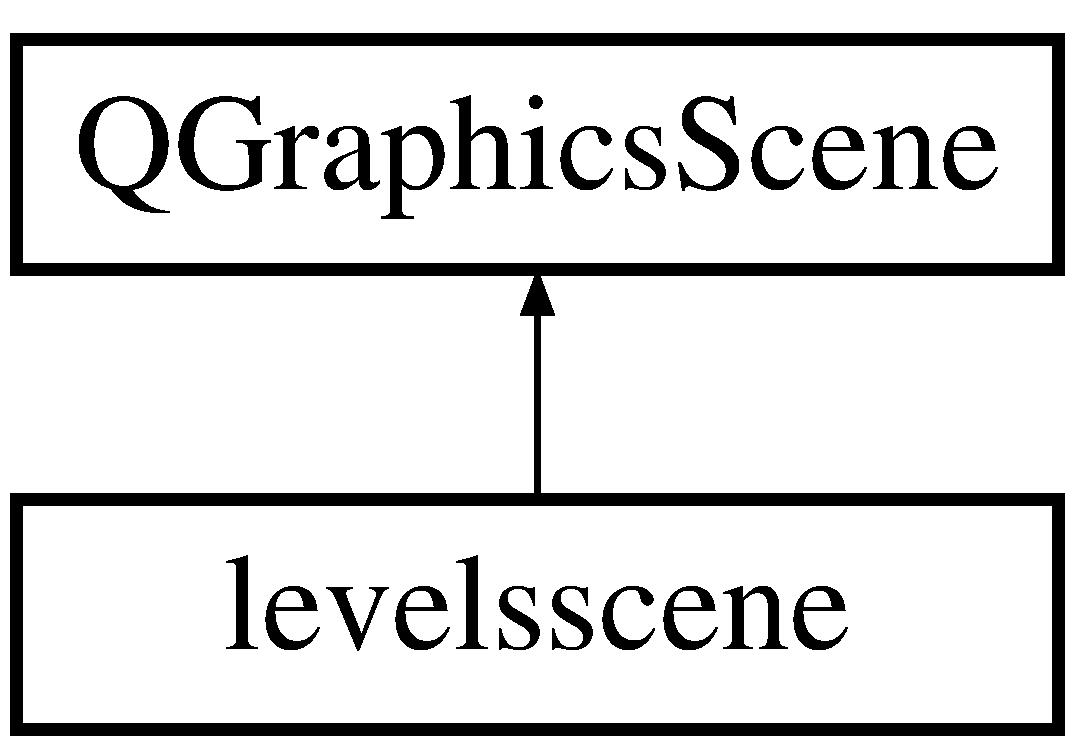
\includegraphics[height=2.000000cm]{classlevelsscene}
\end{center}
\end{figure}
\subsection*{Public Slots}
\begin{DoxyCompactItemize}
\item 
void \hyperlink{classlevelsscene_afb0be60e25586a4c1f4f2c95d8687939}{check\-Answer} ()
\begin{DoxyCompactList}\small\item\em Checking the User's input and moving popeye and the boat accordingly. If the User Clicks on the pick\-Up Spinach cans dissapear. \end{DoxyCompactList}\item 
\hypertarget{classlevelsscene_a2b34314b18b5c7af96a2ba6bb9d74616}{void \hyperlink{classlevelsscene_a2b34314b18b5c7af96a2ba6bb9d74616}{display\-Hint} ()}\label{classlevelsscene_a2b34314b18b5c7af96a2ba6bb9d74616}

\begin{DoxyCompactList}\small\item\em Displaying the 3 hints and repeating them if passed over all of them and decrement score accordingly. \end{DoxyCompactList}\item 
void \hyperlink{classlevelsscene_ae6427d1e5f4207e87dab83a4f9ec6302}{pause\-Level} ()
\begin{DoxyCompactList}\small\item\em Pause the level the user's in. \end{DoxyCompactList}\item 
void \hyperlink{classlevelsscene_a9eb73af70c2c3030be31ba44b5966d20}{retry\-Level} ()
\begin{DoxyCompactList}\small\item\em Retry level and reset positons to initial hard coded positions. \end{DoxyCompactList}\item 
void \hyperlink{classlevelsscene_ab224af4c9e09ba73a8f38345643978b9}{hide\-Scene} ()
\begin{DoxyCompactList}\small\item\em Hide the scene. \end{DoxyCompactList}\item 
void \hyperlink{classlevelsscene_a3fc9fb8b563863ca1f73109a7f94dbba}{update\-Countdown\-Timer} ()
\begin{DoxyCompactList}\small\item\em Function that will update the timer and then display it. \end{DoxyCompactList}\end{DoxyCompactItemize}
\subsection*{Public Member Functions}
\begin{DoxyCompactItemize}
\item 
\hyperlink{classlevelsscene_ac88ccf0616d65eeea4793d9b7f185fe8}{levelsscene} (Q\-String user)
\begin{DoxyCompactList}\small\item\em The constructor the this class is called, everytime the user clicks on the Let's Go! Button and thus, the corresponding level is loaded from the appropriate text file. Each Level have different specs and object that are loaded to their appropriate positions. \end{DoxyCompactList}\item 
\hypertarget{classlevelsscene_aad6a31116f8cf58b8f2240be36843657}{void {\bfseries loose\-Life} ()}\label{classlevelsscene_aad6a31116f8cf58b8f2240be36843657}

\item 
\hypertarget{classlevelsscene_a238d7f1f1542f943fb7851535a83cf52}{void {\bfseries game\-Over} ()}\label{classlevelsscene_a238d7f1f1542f943fb7851535a83cf52}

\item 
void \hyperlink{classlevelsscene_a4b0a1ba6c491db4488cd28a08c18591d}{you\-Lost} (bool)
\begin{DoxyCompactList}\small\item\em Decrementing lifes, score and showing appropriate pop up window when users' looses. \end{DoxyCompactList}\item 
void \hyperlink{classlevelsscene_ab7752c641256cdc4389ad166b421838a}{you\-Won} ()
\begin{DoxyCompactList}\small\item\em Incrementing score, proceeding to the \hyperlink{classgame1scene}{game1scene} and showing appropriate pop up window when user wins. \end{DoxyCompactList}\item 
void \hyperlink{classlevelsscene_ae380900a9cf4e534bd61946861fd350e}{set\-Up\-Countdown\-Timer} ()
\begin{DoxyCompactList}\small\item\em $<$ Timer controlling the countdown \end{DoxyCompactList}\end{DoxyCompactItemize}
\subsection*{Public Attributes}
\begin{DoxyCompactItemize}
\item 
\hypertarget{classlevelsscene_a438c5aa1d42421be740b3ffa2e0f9bac}{Q\-String {\bfseries user}}\label{classlevelsscene_a438c5aa1d42421be740b3ffa2e0f9bac}

\item 
\hypertarget{classlevelsscene_ad56713e7d1bcd6fd0a55ae375b269d19}{\hyperlink{classPopeye}{Popeye} $\ast$ \hyperlink{classlevelsscene_ad56713e7d1bcd6fd0a55ae375b269d19}{popeye} = new \hyperlink{classPopeye}{Popeye}()}\label{classlevelsscene_ad56713e7d1bcd6fd0a55ae375b269d19}

\begin{DoxyCompactList}\small\item\em Creating the references to the Objects. \end{DoxyCompactList}\item 
\hypertarget{classlevelsscene_a172c29c688ab3b992718c126a546bc5d}{\hyperlink{classspinach}{spinach} $\ast$ {\bfseries spinach1} = new \hyperlink{classspinach}{spinach}()}\label{classlevelsscene_a172c29c688ab3b992718c126a546bc5d}

\item 
\hypertarget{classlevelsscene_a47930f9f071ec2554cd259ffdd878b19}{\hyperlink{classspinach}{spinach} $\ast$ {\bfseries spinach2} = new \hyperlink{classspinach}{spinach}()}\label{classlevelsscene_a47930f9f071ec2554cd259ffdd878b19}

\item 
\hypertarget{classlevelsscene_aa7a7a4ed666f12828fc4cc7e5727a4be}{\hyperlink{classspinach}{spinach} $\ast$ {\bfseries spinach3} = new \hyperlink{classspinach}{spinach}()}\label{classlevelsscene_aa7a7a4ed666f12828fc4cc7e5727a4be}

\item 
\hypertarget{classlevelsscene_a2aa538f94ab2a37a21e9cbda55f95fdc}{\hyperlink{classriver}{river} $\ast$ {\bfseries river1} = new \hyperlink{classriver}{river}()}\label{classlevelsscene_a2aa538f94ab2a37a21e9cbda55f95fdc}

\item 
\hypertarget{classlevelsscene_afde2853c70466d2650f2d22a8a38476f}{\hyperlink{classboat}{boat} $\ast$ {\bfseries boat1} = new \hyperlink{classboat}{boat}()}\label{classlevelsscene_afde2853c70466d2650f2d22a8a38476f}

\item 
\hypertarget{classlevelsscene_a3360b5541677c90abe0dc578fa23d9cd}{\hyperlink{classrock}{rock} $\ast$ {\bfseries rock1} = new \hyperlink{classrock}{rock}()}\label{classlevelsscene_a3360b5541677c90abe0dc578fa23d9cd}

\item 
\hypertarget{classlevelsscene_a0ad43dd80f27a36ca3e7199c499322fd}{\hyperlink{classriverObstacle}{river\-Obstacle} $\ast$ {\bfseries obstacle} = new \hyperlink{classriverObstacle}{river\-Obstacle}}\label{classlevelsscene_a0ad43dd80f27a36ca3e7199c499322fd}

\item 
\hypertarget{classlevelsscene_a36a5a006fa44ef570bf00320a50dc6ae}{\hyperlink{classsmallRiver}{small\-River} $\ast$ {\bfseries small\-River1} = new \hyperlink{classsmallRiver}{small\-River}()}\label{classlevelsscene_a36a5a006fa44ef570bf00320a50dc6ae}

\item 
\hypertarget{classlevelsscene_a7362f819c35583c27a1746357f1b2f76}{\hyperlink{classsmallRiver}{small\-River} $\ast$ {\bfseries small\-River2} = new \hyperlink{classsmallRiver}{small\-River}()}\label{classlevelsscene_a7362f819c35583c27a1746357f1b2f76}

\item 
\hypertarget{classlevelsscene_a9bb43edcf6f4c22bf3400a3758578062}{\hyperlink{classlevels}{levels} $\ast$ {\bfseries l}}\label{classlevelsscene_a9bb43edcf6f4c22bf3400a3758578062}

\item 
\hypertarget{classlevelsscene_a5e0a538e398629d89dcc62d620eff88a}{Q\-Push\-Button $\ast$ {\bfseries run}}\label{classlevelsscene_a5e0a538e398629d89dcc62d620eff88a}

\item 
\hypertarget{classlevelsscene_a12e277418e8d7d9e4ef44d931686f1c6}{Q\-Push\-Button $\ast$ {\bfseries hint}}\label{classlevelsscene_a12e277418e8d7d9e4ef44d931686f1c6}

\item 
\hypertarget{classlevelsscene_a603f99a93fc6f8e97c2121ad59480c95}{Q\-Push\-Button $\ast$ {\bfseries pause}}\label{classlevelsscene_a603f99a93fc6f8e97c2121ad59480c95}

\item 
\hypertarget{classlevelsscene_ae01db667588208787b85257483b461f1}{Q\-Push\-Button $\ast$ {\bfseries retry}}\label{classlevelsscene_ae01db667588208787b85257483b461f1}

\item 
\hypertarget{classlevelsscene_a54b0e28d9331156ecbb5184c723dbafe}{Q\-Push\-Button $\ast$ \hyperlink{classlevelsscene_a54b0e28d9331156ecbb5184c723dbafe}{proceed}}\label{classlevelsscene_a54b0e28d9331156ecbb5184c723dbafe}

\begin{DoxyCompactList}\small\item\em Q\-Widgets that will displayed on the screen. \end{DoxyCompactList}\item 
\hypertarget{classlevelsscene_a62b85c060b3cb074bb0974da5d4580e3}{Q\-Text\-Edit $\ast$ {\bfseries text}}\label{classlevelsscene_a62b85c060b3cb074bb0974da5d4580e3}

\item 
\hypertarget{classlevelsscene_a223b1278a33e4a828ae6ad08d703c25a}{Q\-Label $\ast$ {\bfseries instructions}}\label{classlevelsscene_a223b1278a33e4a828ae6ad08d703c25a}

\item 
\hypertarget{classlevelsscene_a49ebdc6c1f0f718aee0fa693c179e3a9}{Q\-Graphics\-Text\-Item $\ast$ {\bfseries count\-Down\-Text}}\label{classlevelsscene_a49ebdc6c1f0f718aee0fa693c179e3a9}

\item 
\hypertarget{classlevelsscene_a1d9581d7120c445327855fb7fa979ec1}{int {\bfseries countdown} = 120}\label{classlevelsscene_a1d9581d7120c445327855fb7fa979ec1}

\item 
\hypertarget{classlevelsscene_a33ff8c59114eb2a898ae03602a03d81d}{Q\-Timer $\ast$ \hyperlink{classlevelsscene_a33ff8c59114eb2a898ae03602a03d81d}{countdown\-Timer}}\label{classlevelsscene_a33ff8c59114eb2a898ae03602a03d81d}

\begin{DoxyCompactList}\small\item\em $<$ value of the countdown at the start of the game that is = to 120 i.\-e. 2 mins for each level \end{DoxyCompactList}\end{DoxyCompactItemize}


\subsection{Constructor \& Destructor Documentation}
\hypertarget{classlevelsscene_ac88ccf0616d65eeea4793d9b7f185fe8}{\index{levelsscene@{levelsscene}!levelsscene@{levelsscene}}
\index{levelsscene@{levelsscene}!levelsscene@{levelsscene}}
\subsubsection[{levelsscene}]{\setlength{\rightskip}{0pt plus 5cm}levelsscene\-::levelsscene (
\begin{DoxyParamCaption}
\item[{Q\-String}]{user}
\end{DoxyParamCaption}
)}}\label{classlevelsscene_ac88ccf0616d65eeea4793d9b7f185fe8}


The constructor the this class is called, everytime the user clicks on the Let's Go! Button and thus, the corresponding level is loaded from the appropriate text file. Each Level have different specs and object that are loaded to their appropriate positions. 

$<$ User can only pause after level 1 is completed

$<$ if the levels has ot not other spinach cans 

\subsection{Member Function Documentation}
\hypertarget{classlevelsscene_afb0be60e25586a4c1f4f2c95d8687939}{\index{levelsscene@{levelsscene}!check\-Answer@{check\-Answer}}
\index{check\-Answer@{check\-Answer}!levelsscene@{levelsscene}}
\subsubsection[{check\-Answer}]{\setlength{\rightskip}{0pt plus 5cm}void levelsscene\-::check\-Answer (
\begin{DoxyParamCaption}
{}
\end{DoxyParamCaption}
)\hspace{0.3cm}{\ttfamily [slot]}}}\label{classlevelsscene_afb0be60e25586a4c1f4f2c95d8687939}


Checking the User's input and moving popeye and the boat accordingly. If the User Clicks on the pick\-Up Spinach cans dissapear. 

$<$ Run push button function

$<$direction of movement, 0 to the right and anticlockwise

$<$check the argument of the Repeat(args) from the user

$<$get the number of iterations

$<$start reading after we get the number of iterations

$<$ iterate j times over the user's Code

$<$ i is either = 0 or 2 and at the end of the first for loop i is reseted to 2 if there is repetition

popeye cannot move in level 5; boat collides with him only

to check if popeye can pass on the bridge or if there is a river

$<$If popeye collides with the boat, they should both move in the same manner if Boat.\-Move is inputed

$<$In level 7 the boat can only move on a horizontal line

$<$ Each Rotate will rotate popeye by 90 degrees

$<$if the colliding object is of type spinach

$<$ decrement the number of lifes before showing it to the user and show appropriate syntax error \hypertarget{classlevelsscene_ab224af4c9e09ba73a8f38345643978b9}{\index{levelsscene@{levelsscene}!hide\-Scene@{hide\-Scene}}
\index{hide\-Scene@{hide\-Scene}!levelsscene@{levelsscene}}
\subsubsection[{hide\-Scene}]{\setlength{\rightskip}{0pt plus 5cm}void levelsscene\-::hide\-Scene (
\begin{DoxyParamCaption}
{}
\end{DoxyParamCaption}
)\hspace{0.3cm}{\ttfamily [slot]}}}\label{classlevelsscene_ab224af4c9e09ba73a8f38345643978b9}


Hide the scene. 

Hide the levelsscene. \hypertarget{classlevelsscene_ae6427d1e5f4207e87dab83a4f9ec6302}{\index{levelsscene@{levelsscene}!pause\-Level@{pause\-Level}}
\index{pause\-Level@{pause\-Level}!levelsscene@{levelsscene}}
\subsubsection[{pause\-Level}]{\setlength{\rightskip}{0pt plus 5cm}void levelsscene\-::pause\-Level (
\begin{DoxyParamCaption}
{}
\end{DoxyParamCaption}
)\hspace{0.3cm}{\ttfamily [slot]}}}\label{classlevelsscene_ae6427d1e5f4207e87dab83a4f9ec6302}


Pause the level the user's in. 

$<$Since everything is loaded from the text file; the lives, scores, timer and level number, the pause simply closes the scene and when the user re-\/logs in, he just continues where he left off when he clicks on the Let's Start! button \hypertarget{classlevelsscene_a9eb73af70c2c3030be31ba44b5966d20}{\index{levelsscene@{levelsscene}!retry\-Level@{retry\-Level}}
\index{retry\-Level@{retry\-Level}!levelsscene@{levelsscene}}
\subsubsection[{retry\-Level}]{\setlength{\rightskip}{0pt plus 5cm}void levelsscene\-::retry\-Level (
\begin{DoxyParamCaption}
{}
\end{DoxyParamCaption}
)\hspace{0.3cm}{\ttfamily [slot]}}}\label{classlevelsscene_a9eb73af70c2c3030be31ba44b5966d20}


Retry level and reset positons to initial hard coded positions. 

$<$retry -\/$>$ reset popeye's position

$<$ if the levels has ot not other spinach cans \hypertarget{classlevelsscene_ae380900a9cf4e534bd61946861fd350e}{\index{levelsscene@{levelsscene}!set\-Up\-Countdown\-Timer@{set\-Up\-Countdown\-Timer}}
\index{set\-Up\-Countdown\-Timer@{set\-Up\-Countdown\-Timer}!levelsscene@{levelsscene}}
\subsubsection[{set\-Up\-Countdown\-Timer}]{\setlength{\rightskip}{0pt plus 5cm}void levelsscene\-::set\-Up\-Countdown\-Timer (
\begin{DoxyParamCaption}
{}
\end{DoxyParamCaption}
)}}\label{classlevelsscene_ae380900a9cf4e534bd61946861fd350e}


$<$ Timer controlling the countdown 

Initializes Text\-Item that indicates the Countdown at the start of each level.

Setting up the timer \hypertarget{classlevelsscene_a3fc9fb8b563863ca1f73109a7f94dbba}{\index{levelsscene@{levelsscene}!update\-Countdown\-Timer@{update\-Countdown\-Timer}}
\index{update\-Countdown\-Timer@{update\-Countdown\-Timer}!levelsscene@{levelsscene}}
\subsubsection[{update\-Countdown\-Timer}]{\setlength{\rightskip}{0pt plus 5cm}void levelsscene\-::update\-Countdown\-Timer (
\begin{DoxyParamCaption}
{}
\end{DoxyParamCaption}
)\hspace{0.3cm}{\ttfamily [slot]}}}\label{classlevelsscene_a3fc9fb8b563863ca1f73109a7f94dbba}


Function that will update the timer and then display it. 

update S\-L\-O\-T that controls the Countdown to display it when adjusted, every second \hypertarget{classlevelsscene_a4b0a1ba6c491db4488cd28a08c18591d}{\index{levelsscene@{levelsscene}!you\-Lost@{you\-Lost}}
\index{you\-Lost@{you\-Lost}!levelsscene@{levelsscene}}
\subsubsection[{you\-Lost}]{\setlength{\rightskip}{0pt plus 5cm}void levelsscene\-::you\-Lost (
\begin{DoxyParamCaption}
\item[{bool}]{time\-Is\-Up}
\end{DoxyParamCaption}
)}}\label{classlevelsscene_a4b0a1ba6c491db4488cd28a08c18591d}


Decrementing lifes, score and showing appropriate pop up window when users' looses. 

$<$reset the user to level 1

$<$reset the user to level 1 \hypertarget{classlevelsscene_ab7752c641256cdc4389ad166b421838a}{\index{levelsscene@{levelsscene}!you\-Won@{you\-Won}}
\index{you\-Won@{you\-Won}!levelsscene@{levelsscene}}
\subsubsection[{you\-Won}]{\setlength{\rightskip}{0pt plus 5cm}void levelsscene\-::you\-Won (
\begin{DoxyParamCaption}
{}
\end{DoxyParamCaption}
)}}\label{classlevelsscene_ab7752c641256cdc4389ad166b421838a}


Incrementing score, proceeding to the \hyperlink{classgame1scene}{game1scene} and showing appropriate pop up window when user wins. 

$<$Increment the score according the count of lifes, the higher the lifes, the higher the score

$<$ Increment the score according to the player's time 

The documentation for this class was generated from the following files\-:\begin{DoxyCompactItemize}
\item 
levelsscene.\-h\item 
\hyperlink{levelsscene_8cpp}{levelsscene.\-cpp}\end{DoxyCompactItemize}

\hypertarget{classLifeCounter}{\section{Life\-Counter Class Reference}
\label{classLifeCounter}\index{Life\-Counter@{Life\-Counter}}
}
Inheritance diagram for Life\-Counter\-:\begin{figure}[H]
\begin{center}
\leavevmode
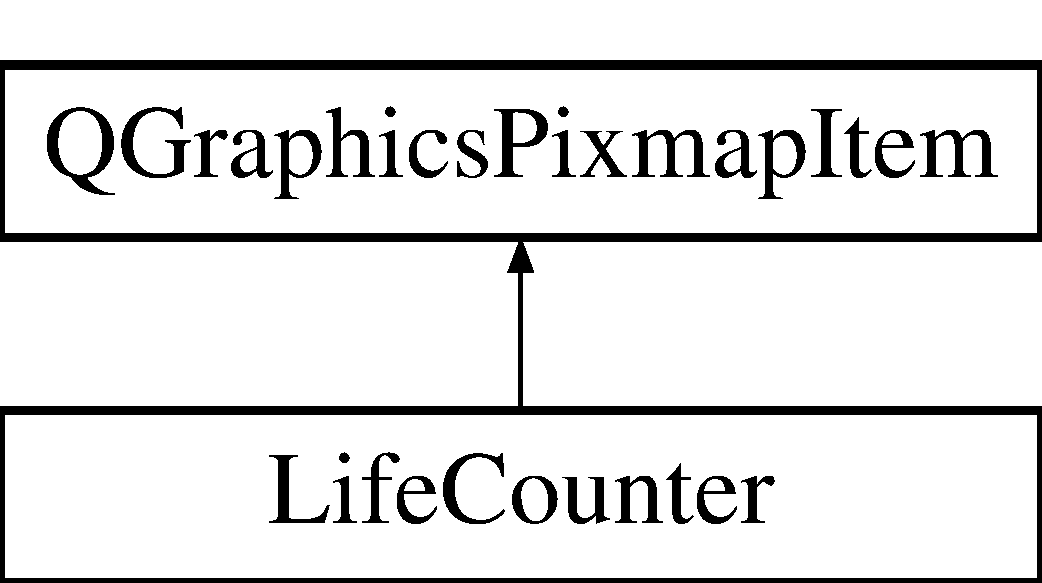
\includegraphics[height=2.000000cm]{classLifeCounter}
\end{center}
\end{figure}
\subsection*{Public Member Functions}
\begin{DoxyCompactItemize}
\item 
\hypertarget{classLifeCounter_a855f3024526e01622a4e2cdc7700b1ff}{\hyperlink{classLifeCounter_a855f3024526e01622a4e2cdc7700b1ff}{Life\-Counter} (int life)}\label{classLifeCounter_a855f3024526e01622a4e2cdc7700b1ff}

\begin{DoxyCompactList}\small\item\em Constructor. \end{DoxyCompactList}\end{DoxyCompactItemize}


The documentation for this class was generated from the following files\-:\begin{DoxyCompactItemize}
\item 
\hyperlink{lifecounter_8h}{lifecounter.\-h}\item 
\hyperlink{lifecounter_8cpp}{lifecounter.\-cpp}\end{DoxyCompactItemize}

\hypertarget{classlocks}{\section{locks Class Reference}
\label{classlocks}\index{locks@{locks}}
}
Inheritance diagram for locks\-:\begin{figure}[H]
\begin{center}
\leavevmode
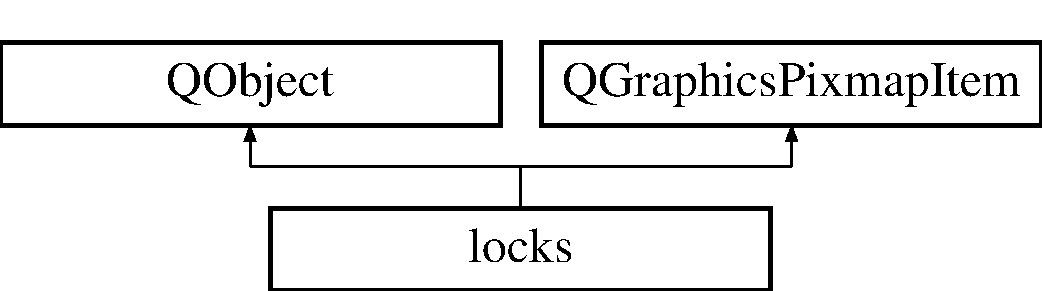
\includegraphics[height=2.000000cm]{classlocks}
\end{center}
\end{figure}
\subsection*{Public Member Functions}
\begin{DoxyCompactItemize}
\item 
\hypertarget{classlocks_a66bc229b3a60f6baa5d3f34f218a5114}{\hyperlink{classlocks_a66bc229b3a60f6baa5d3f34f218a5114}{locks} (Q\-Object $\ast$parent=nullptr)}\label{classlocks_a66bc229b3a60f6baa5d3f34f218a5114}

\begin{DoxyCompactList}\small\item\em Setting the lock Image. \end{DoxyCompactList}\end{DoxyCompactItemize}


The documentation for this class was generated from the following files\-:\begin{DoxyCompactItemize}
\item 
\hyperlink{locks_8h}{locks.\-h}\item 
\hyperlink{locks_8cpp}{locks.\-cpp}\end{DoxyCompactItemize}

\hypertarget{classloggInWidget}{\section{logg\-In\-Widget Class Reference}
\label{classloggInWidget}\index{logg\-In\-Widget@{logg\-In\-Widget}}
}
Inheritance diagram for logg\-In\-Widget\-:\begin{figure}[H]
\begin{center}
\leavevmode
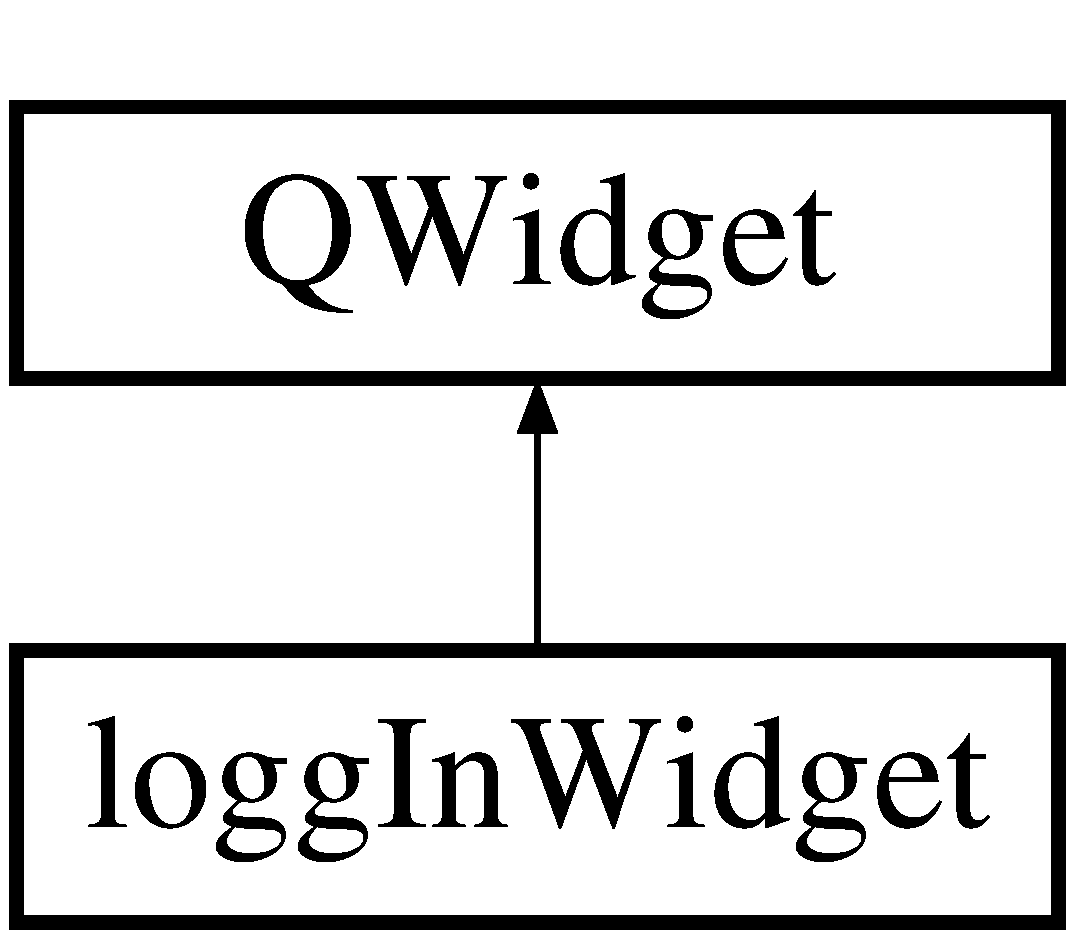
\includegraphics[height=2.000000cm]{classloggInWidget}
\end{center}
\end{figure}
\subsection*{Public Slots}
\begin{DoxyCompactItemize}
\item 
\hypertarget{classloggInWidget_abcc1aa0d2f8ecdee120a3b0461086ce0}{void {\bfseries start\-Games} ()}\label{classloggInWidget_abcc1aa0d2f8ecdee120a3b0461086ce0}

\end{DoxyCompactItemize}
\subsection*{Public Member Functions}
\begin{DoxyCompactItemize}
\item 
\hypertarget{classloggInWidget_a04dcda82efc89df69c734e5077ad564e}{{\bfseries logg\-In\-Widget} (Q\-String user=\char`\"{}guest\char`\"{})}\label{classloggInWidget_a04dcda82efc89df69c734e5077ad564e}

\item 
\hypertarget{classloggInWidget_ab3c883a2d4741be42d58bc2841b19d4c}{void {\bfseries set\-Vertical\-Layout} ()}\label{classloggInWidget_ab3c883a2d4741be42d58bc2841b19d4c}

\item 
\hypertarget{classloggInWidget_a3c068d2539ba9a9932d5144d6b0888bc}{void {\bfseries set\-Grid\-Layout} ()}\label{classloggInWidget_a3c068d2539ba9a9932d5144d6b0888bc}

\end{DoxyCompactItemize}
\subsection*{Public Attributes}
\begin{DoxyCompactItemize}
\item 
\hypertarget{classloggInWidget_a993b2cb5c5a849fbd52247c73217f0e4}{Q\-Label $\ast$ {\bfseries user\-Name}}\label{classloggInWidget_a993b2cb5c5a849fbd52247c73217f0e4}

\item 
\hypertarget{classloggInWidget_a3a96d17dbd0ef6c867bd9e974cd1e099}{Q\-Label $\ast$ {\bfseries log\-In}}\label{classloggInWidget_a3a96d17dbd0ef6c867bd9e974cd1e099}

\item 
\hypertarget{classloggInWidget_a51725943ce38347537ad933b0d12a456}{Q\-Push\-Button $\ast$ {\bfseries games}}\label{classloggInWidget_a51725943ce38347537ad933b0d12a456}

\item 
\hypertarget{classloggInWidget_a4acf8b02bcc79d610be1211d142fe7e0}{Q\-String {\bfseries user}}\label{classloggInWidget_a4acf8b02bcc79d610be1211d142fe7e0}

\item 
\hypertarget{classloggInWidget_a57d62601628a5766a2f910ddd7f945f8}{Q\-V\-Box\-Layout $\ast$ {\bfseries Vertical\-L}}\label{classloggInWidget_a57d62601628a5766a2f910ddd7f945f8}

\item 
\hypertarget{classloggInWidget_a605b4324830843e3f51201dcec9bd042}{Q\-Grid\-Layout $\ast$ {\bfseries Grid\-L}}\label{classloggInWidget_a605b4324830843e3f51201dcec9bd042}

\end{DoxyCompactItemize}


The documentation for this class was generated from the following files\-:\begin{DoxyCompactItemize}
\item 
logginwidget.\-h\item 
logginwidget.\-cpp\item 
logginwidget.\-cpp.\-B\-A\-C\-K\-U\-P.\-3062.\-cpp\item 
logginwidget.\-cpp.\-B\-A\-S\-E.\-3062.\-cpp\item 
logginwidget.\-cpp.\-L\-O\-C\-A\-L.\-3062.\-cpp\item 
logginwidget.\-cpp.\-R\-E\-M\-O\-T\-E.\-3062.\-cpp\end{DoxyCompactItemize}

\hypertarget{classLogOnWidget}{\section{Log\-On\-Widget Class Reference}
\label{classLogOnWidget}\index{Log\-On\-Widget@{Log\-On\-Widget}}
}
Inheritance diagram for Log\-On\-Widget\-:\begin{figure}[H]
\begin{center}
\leavevmode
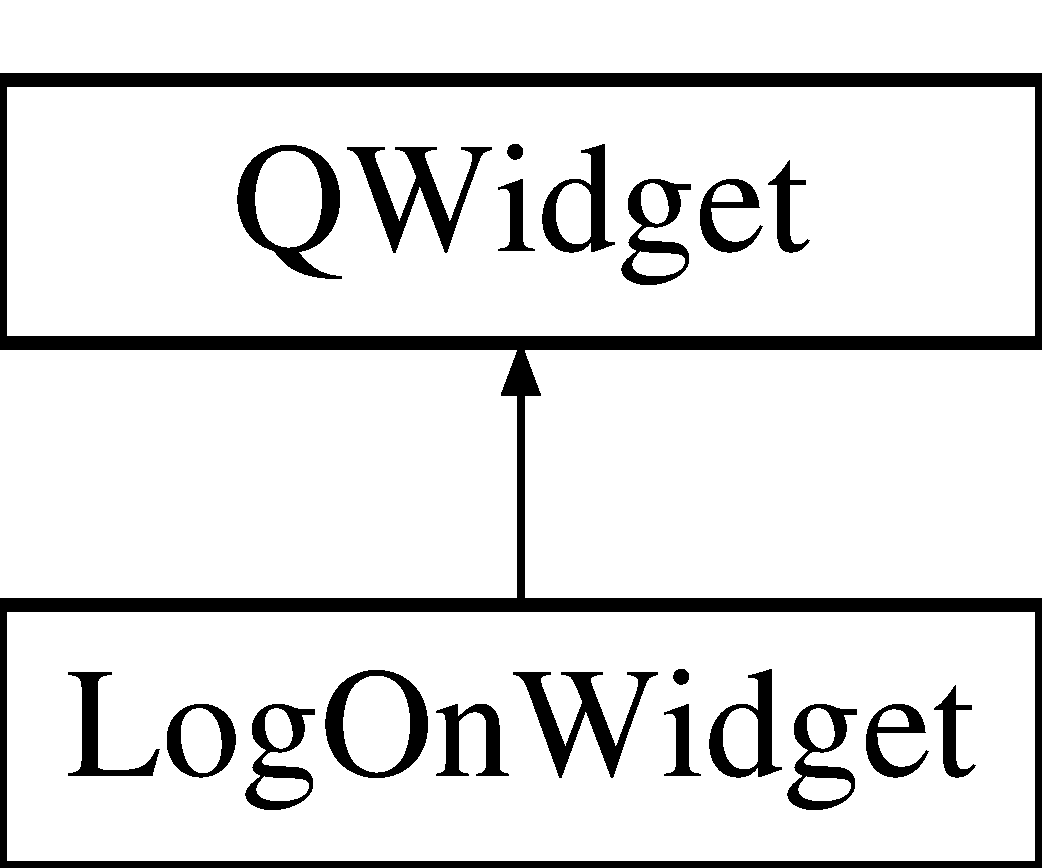
\includegraphics[height=2.000000cm]{classLogOnWidget}
\end{center}
\end{figure}
\subsection*{Public Slots}
\begin{DoxyCompactItemize}
\item 
\hypertarget{classLogOnWidget_a8954686daf8ae217858582249e8d12e5}{void {\bfseries Goto\-Sign\-Up\-Page} ()}\label{classLogOnWidget_a8954686daf8ae217858582249e8d12e5}

\item 
\hypertarget{classLogOnWidget_a650ea5d3139aa86728006cbd3e865f26}{void {\bfseries Log\-In\-As\-Guest} ()}\label{classLogOnWidget_a650ea5d3139aa86728006cbd3e865f26}

\item 
\hypertarget{classLogOnWidget_aefc58cfadb68a5ef7b57bc47a9c90622}{void {\bfseries Goto\-Sign\-In\-Page} ()}\label{classLogOnWidget_aefc58cfadb68a5ef7b57bc47a9c90622}

\end{DoxyCompactItemize}
\subsection*{Public Member Functions}
\begin{DoxyCompactItemize}
\item 
\hypertarget{classLogOnWidget_afae1360f1879334a759db2e3a9aa3037}{{\bfseries Log\-On\-Widget} (Q\-Widget $\ast$parent=nullptr)}\label{classLogOnWidget_afae1360f1879334a759db2e3a9aa3037}

\item 
\hypertarget{classLogOnWidget_aa2da3f5ed0e5a22511e197b8446700ca}{void {\bfseries set\-Vertical\-Layout} ()}\label{classLogOnWidget_aa2da3f5ed0e5a22511e197b8446700ca}

\item 
\hypertarget{classLogOnWidget_ad8b097280c12841ce3e2ce6a4d6a847f}{void {\bfseries set\-Grid\-Layout} ()}\label{classLogOnWidget_ad8b097280c12841ce3e2ce6a4d6a847f}

\end{DoxyCompactItemize}
\subsection*{Public Attributes}
\begin{DoxyCompactItemize}
\item 
\hypertarget{classLogOnWidget_a278b4aef2ed697a807caf122765bba14}{Q\-Push\-Button $\ast$ {\bfseries Sign\-Up\-Button}}\label{classLogOnWidget_a278b4aef2ed697a807caf122765bba14}

\item 
\hypertarget{classLogOnWidget_a03c8de69df4213f5c20ccb85e0bac36a}{Q\-Push\-Button $\ast$ {\bfseries Sign\-In\-Button}}\label{classLogOnWidget_a03c8de69df4213f5c20ccb85e0bac36a}

\item 
\hypertarget{classLogOnWidget_ab102bcf828c0221a21b541c864ea452c}{Q\-Push\-Button $\ast$ {\bfseries Guest\-Button}}\label{classLogOnWidget_ab102bcf828c0221a21b541c864ea452c}

\item 
\hypertarget{classLogOnWidget_acd4a39c90fb3fb618d0bd69a5af7b856}{Q\-Label $\ast$ {\bfseries Title\-Label}}\label{classLogOnWidget_acd4a39c90fb3fb618d0bd69a5af7b856}

\item 
\hypertarget{classLogOnWidget_a91f18d4e66949d4e689195a53f840272}{Q\-Label $\ast$ {\bfseries Info\-Label}}\label{classLogOnWidget_a91f18d4e66949d4e689195a53f840272}

\item 
\hypertarget{classLogOnWidget_a55af2f5d84c099c242635dc057fea89c}{Q\-V\-Box\-Layout $\ast$ {\bfseries Vertical\-Layout}}\label{classLogOnWidget_a55af2f5d84c099c242635dc057fea89c}

\item 
\hypertarget{classLogOnWidget_aa2f97eb976a762dfef72222e70fc9d2f}{Q\-Grid\-Layout $\ast$ {\bfseries Grid\-Layout}}\label{classLogOnWidget_aa2f97eb976a762dfef72222e70fc9d2f}

\item 
\hypertarget{classLogOnWidget_a73d767c2ed43e2327c8200307f73657d}{Q\-Graphics\-Scene $\ast$ {\bfseries Scene}}\label{classLogOnWidget_a73d767c2ed43e2327c8200307f73657d}

\end{DoxyCompactItemize}


The documentation for this class was generated from the following files\-:\begin{DoxyCompactItemize}
\item 
logonwidget.\-h\item 
logonwidget.\-cpp\end{DoxyCompactItemize}

\hypertarget{classlost}{\section{lost Class Reference}
\label{classlost}\index{lost@{lost}}
}
Inheritance diagram for lost\-:\begin{figure}[H]
\begin{center}
\leavevmode
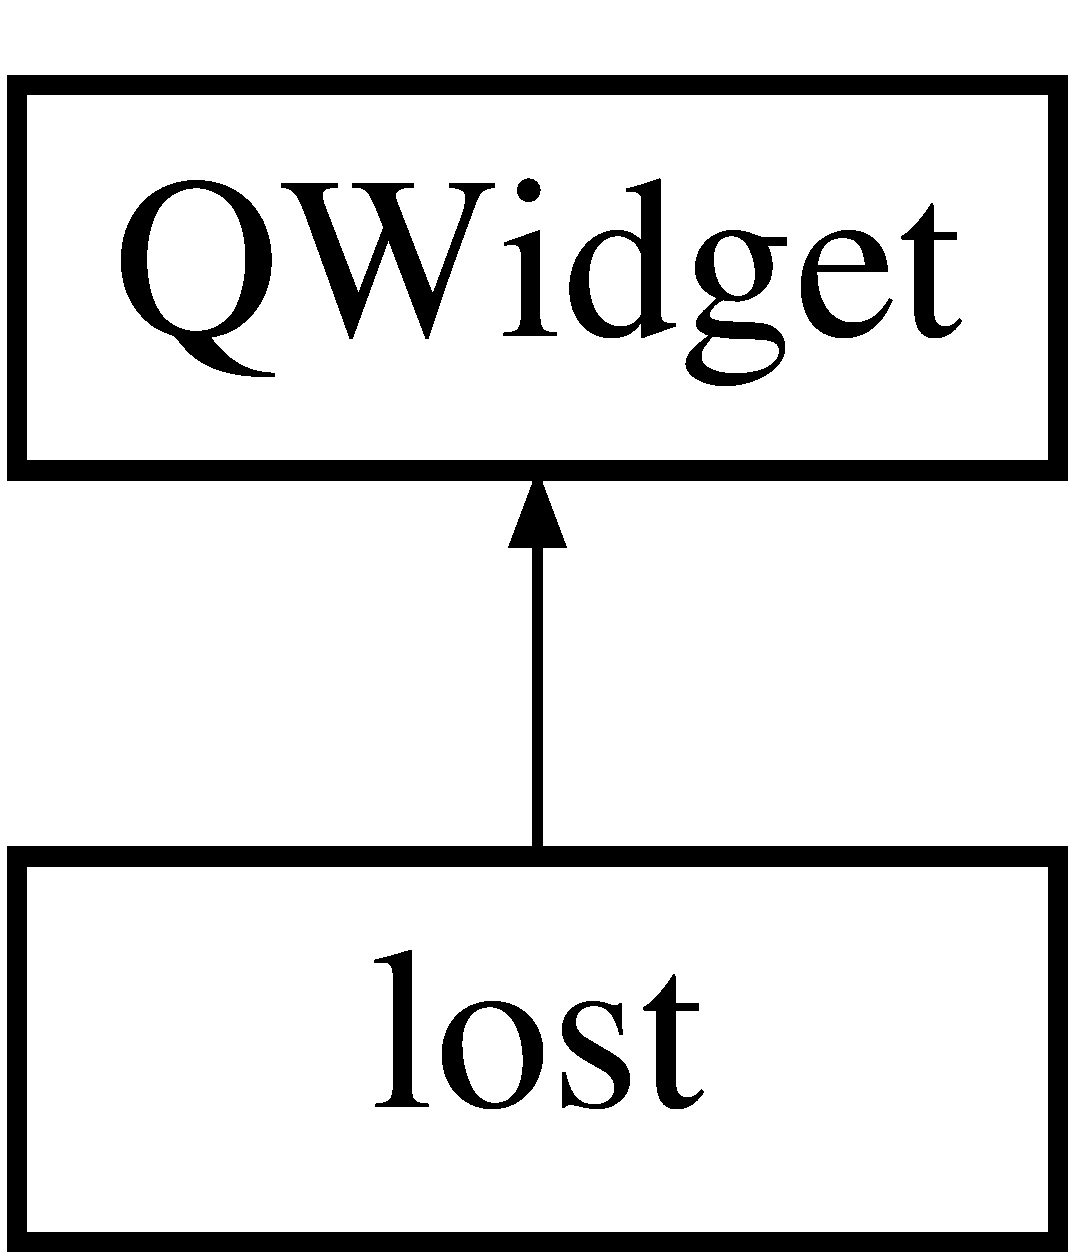
\includegraphics[height=2.000000cm]{classlost}
\end{center}
\end{figure}
\subsection*{Public Member Functions}
\begin{DoxyCompactItemize}
\item 
\hypertarget{classlost_ab0f3e550330f6431091188db0a27d559}{\hyperlink{classlost_ab0f3e550330f6431091188db0a27d559}{lost} (Q\-Widget $\ast$parent=nullptr)}\label{classlost_ab0f3e550330f6431091188db0a27d559}

\begin{DoxyCompactList}\small\item\em Setting the lost pop up window content, displaying the total number of lifes left and any syntax error when needed. \end{DoxyCompactList}\item 
\hyperlink{classlost_ac722377b01564776ab8f9e3b4ae000ce}{lost} (int lifes, Q\-Widget $\ast$parent=nullptr)
\item 
\hyperlink{classlost_ab4341492387749792920ce0e93cb7684}{lost} (int lifes, Q\-String command, Q\-Widget $\ast$parent=nullptr)
\end{DoxyCompactItemize}


\subsection{Constructor \& Destructor Documentation}
\hypertarget{classlost_ac722377b01564776ab8f9e3b4ae000ce}{\index{lost@{lost}!lost@{lost}}
\index{lost@{lost}!lost@{lost}}
\subsubsection[{lost}]{\setlength{\rightskip}{0pt plus 5cm}lost\-::lost (
\begin{DoxyParamCaption}
\item[{int}]{lifes, }
\item[{Q\-Widget $\ast$}]{parent = {\ttfamily nullptr}}
\end{DoxyParamCaption}
)}}\label{classlost_ac722377b01564776ab8f9e3b4ae000ce}
$<$If the lives count is less than 0 the user would have lost completely and therefore would have to restart the game \hypertarget{classlost_ab4341492387749792920ce0e93cb7684}{\index{lost@{lost}!lost@{lost}}
\index{lost@{lost}!lost@{lost}}
\subsubsection[{lost}]{\setlength{\rightskip}{0pt plus 5cm}lost\-::lost (
\begin{DoxyParamCaption}
\item[{int}]{lifes, }
\item[{Q\-String}]{command, }
\item[{Q\-Widget $\ast$}]{parent = {\ttfamily nullptr}}
\end{DoxyParamCaption}
)}}\label{classlost_ab4341492387749792920ce0e93cb7684}
$<$ not checking for the in entered in the Move(\#) function 

The documentation for this class was generated from the following files\-:\begin{DoxyCompactItemize}
\item 
\hyperlink{lost_8h}{lost.\-h}\item 
\hyperlink{lost_8cpp}{lost.\-cpp}\end{DoxyCompactItemize}

\hypertarget{classminiBug}{\section{mini\-Bug Class Reference}
\label{classminiBug}\index{mini\-Bug@{mini\-Bug}}
}
Inheritance diagram for mini\-Bug\-:\begin{figure}[H]
\begin{center}
\leavevmode
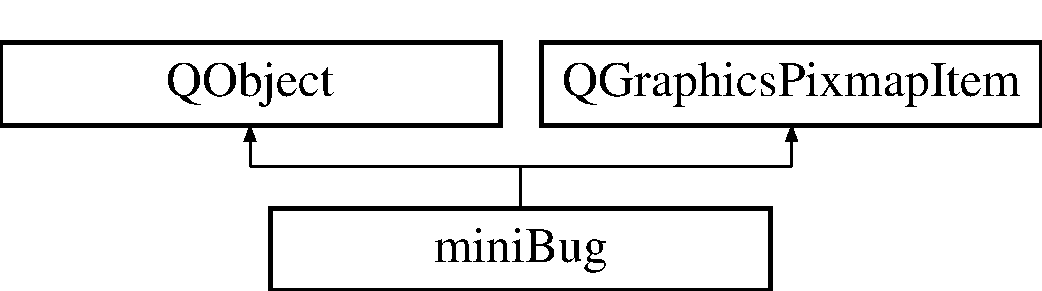
\includegraphics[height=2.000000cm]{classminiBug}
\end{center}
\end{figure}
\subsection*{Public Slots}
\begin{DoxyCompactItemize}
\item 
\hypertarget{classminiBug_a990a1d581da44901dd81386e4196a766}{void \hyperlink{classminiBug_a990a1d581da44901dd81386e4196a766}{move} ()}\label{classminiBug_a990a1d581da44901dd81386e4196a766}

\begin{DoxyCompactList}\small\item\em responsible of moving the \hyperlink{classminiBug}{mini\-Bug} on each timer timeout \end{DoxyCompactList}\end{DoxyCompactItemize}
\subsection*{Public Member Functions}
\begin{DoxyCompactItemize}
\item 
\hypertarget{classminiBug_a38ba11cf31a4539b7d2993370bfe92a7}{\hyperlink{classminiBug_a38ba11cf31a4539b7d2993370bfe92a7}{mini\-Bug} (\hyperlink{classGame2Scene}{Game2\-Scene} $\ast$, \hyperlink{classBug}{Bug} $\ast$, int)}\label{classminiBug_a38ba11cf31a4539b7d2993370bfe92a7}

\begin{DoxyCompactList}\small\item\em Constructor. \end{DoxyCompactList}\end{DoxyCompactItemize}
\subsection*{Public Attributes}
\begin{DoxyCompactItemize}
\item 
\hypertarget{classminiBug_ab360b707ed5e40c2a74e3a8eabaf8514}{Q\-Pixmap $\ast$ \hyperlink{classminiBug_ab360b707ed5e40c2a74e3a8eabaf8514}{icon}}\label{classminiBug_ab360b707ed5e40c2a74e3a8eabaf8514}

\begin{DoxyCompactList}\small\item\em Pixmap holding the image. \end{DoxyCompactList}\item 
\hypertarget{classminiBug_ae013b5a05edb52ba47303fa601bac4a6}{\hyperlink{classGame2Scene}{Game2\-Scene} $\ast$ \hyperlink{classminiBug_ae013b5a05edb52ba47303fa601bac4a6}{scene}}\label{classminiBug_ae013b5a05edb52ba47303fa601bac4a6}

\begin{DoxyCompactList}\small\item\em The scene where the \hyperlink{classminiBug}{mini\-Bug} is located. \end{DoxyCompactList}\item 
\hypertarget{classminiBug_aa4f549ded50743ab672687685da28250}{\hyperlink{classBug}{Bug} $\ast$ \hyperlink{classminiBug_aa4f549ded50743ab672687685da28250}{bug}}\label{classminiBug_aa4f549ded50743ab672687685da28250}

\begin{DoxyCompactList}\small\item\em The parent \hyperlink{classBug}{Bug}. \end{DoxyCompactList}\item 
\hypertarget{classminiBug_a3e213df3a33778cf561e8eda60c5b43b}{Q\-Timer $\ast$ \hyperlink{classminiBug_a3e213df3a33778cf561e8eda60c5b43b}{timer}}\label{classminiBug_a3e213df3a33778cf561e8eda60c5b43b}

\begin{DoxyCompactList}\small\item\em Q\-Timer used to move the \hyperlink{classminiBug}{mini\-Bug} periodically. \end{DoxyCompactList}\item 
\hypertarget{classminiBug_a77b0631d176aba6eab8f7127b34e0e46}{int \hyperlink{classminiBug_a77b0631d176aba6eab8f7127b34e0e46}{steps}}\label{classminiBug_a77b0631d176aba6eab8f7127b34e0e46}

\begin{DoxyCompactList}\small\item\em Number of steps taken already used in determining the range. \end{DoxyCompactList}\item 
\hypertarget{classminiBug_a41ac911a268d263e14ab345b1376d53a}{int \hyperlink{classminiBug_a41ac911a268d263e14ab345b1376d53a}{dir}}\label{classminiBug_a41ac911a268d263e14ab345b1376d53a}

\begin{DoxyCompactList}\small\item\em Integer holding the direction of the \hyperlink{classminiBug}{mini\-Bug}. \end{DoxyCompactList}\end{DoxyCompactItemize}


The documentation for this class was generated from the following files\-:\begin{DoxyCompactItemize}
\item 
minibug.\-h\item 
\hyperlink{minibug_8cpp}{minibug.\-cpp}\end{DoxyCompactItemize}

\hypertarget{classPopeye}{\section{Popeye Class Reference}
\label{classPopeye}\index{Popeye@{Popeye}}
}
Inheritance diagram for Popeye\-:\begin{figure}[H]
\begin{center}
\leavevmode
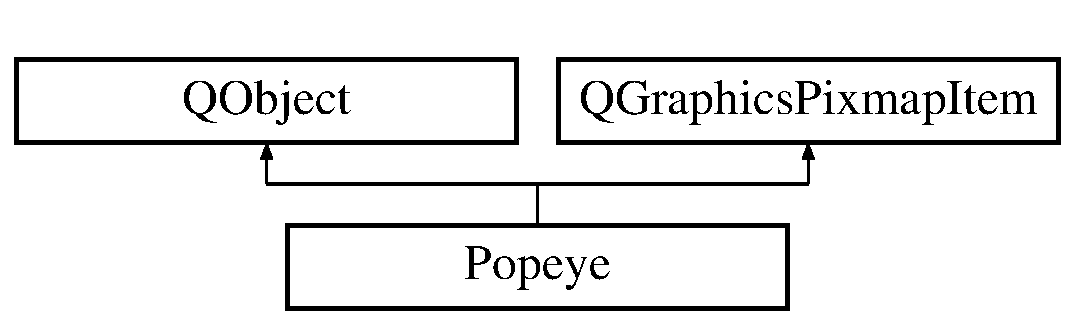
\includegraphics[height=2.000000cm]{classPopeye}
\end{center}
\end{figure}
\subsection*{Public Member Functions}
\begin{DoxyCompactItemize}
\item 
\hypertarget{classPopeye_ae4a4d6f5e847b9b316067130239c47f9}{\hyperlink{classPopeye_ae4a4d6f5e847b9b316067130239c47f9}{Popeye} (Q\-Object $\ast$parent=nullptr)}\label{classPopeye_ae4a4d6f5e847b9b316067130239c47f9}

\begin{DoxyCompactList}\small\item\em Setting \hyperlink{classPopeye}{Popeye}'s Image. \end{DoxyCompactList}\item 
\hypertarget{classPopeye_a9d6721f8f275b6eb1747408fa292cd71}{void {\bfseries collision} ()}\label{classPopeye_a9d6721f8f275b6eb1747408fa292cd71}

\end{DoxyCompactItemize}


The documentation for this class was generated from the following files\-:\begin{DoxyCompactItemize}
\item 
\hyperlink{popeye_8h}{popeye.\-h}\item 
\hyperlink{popeye_8cpp}{popeye.\-cpp}\end{DoxyCompactItemize}

\hypertarget{classQualityControlIcon}{\section{Quality\-Control\-Icon Class Reference}
\label{classQualityControlIcon}\index{Quality\-Control\-Icon@{Quality\-Control\-Icon}}
}
Inheritance diagram for Quality\-Control\-Icon\-:\begin{figure}[H]
\begin{center}
\leavevmode
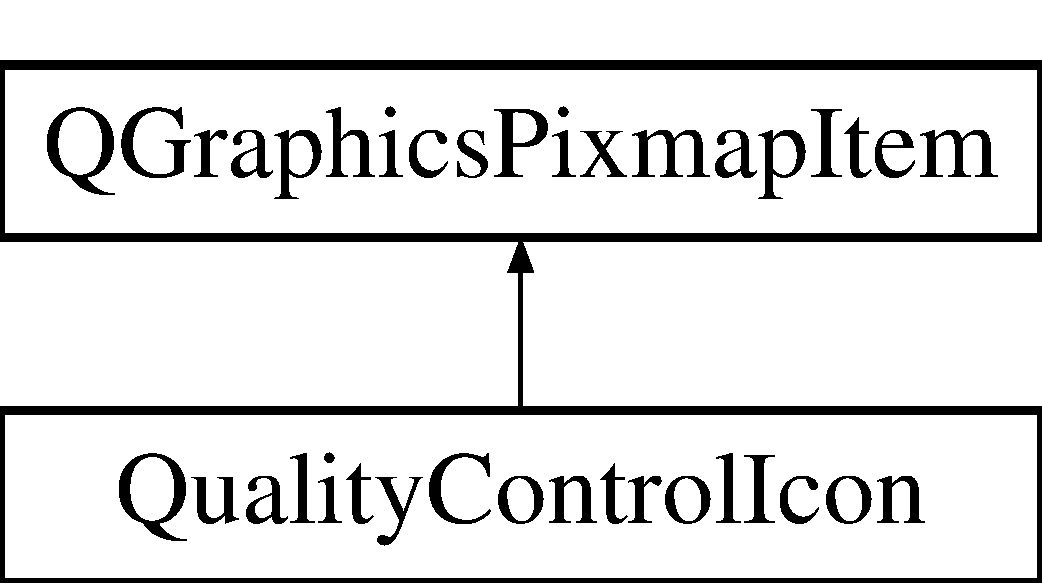
\includegraphics[height=2.000000cm]{classQualityControlIcon}
\end{center}
\end{figure}
\subsection*{Public Member Functions}
\begin{DoxyCompactItemize}
\item 
\hypertarget{classQualityControlIcon_abc6bd22cb8fd253c3f777b7e0a970569}{\hyperlink{classQualityControlIcon_abc6bd22cb8fd253c3f777b7e0a970569}{Quality\-Control\-Icon} ()}\label{classQualityControlIcon_abc6bd22cb8fd253c3f777b7e0a970569}

\begin{DoxyCompactList}\small\item\em Constructor. \end{DoxyCompactList}\end{DoxyCompactItemize}
\subsection*{Public Attributes}
\begin{DoxyCompactItemize}
\item 
\hypertarget{classQualityControlIcon_a0b31fdbf5db70c271d23055cfb64190d}{Q\-Pixmap $\ast$ \hyperlink{classQualityControlIcon_a0b31fdbf5db70c271d23055cfb64190d}{icon}}\label{classQualityControlIcon_a0b31fdbf5db70c271d23055cfb64190d}

\begin{DoxyCompactList}\small\item\em Pixmap holding the image of the Q\-C icon. \end{DoxyCompactList}\end{DoxyCompactItemize}


The documentation for this class was generated from the following files\-:\begin{DoxyCompactItemize}
\item 
\hyperlink{qualitycontrolicon_8h}{qualitycontrolicon.\-h}\item 
\hyperlink{qualitycontrolicon_8cpp}{qualitycontrolicon.\-cpp}\end{DoxyCompactItemize}

\hypertarget{classriver}{\section{river Class Reference}
\label{classriver}\index{river@{river}}
}
Inheritance diagram for river\-:\begin{figure}[H]
\begin{center}
\leavevmode
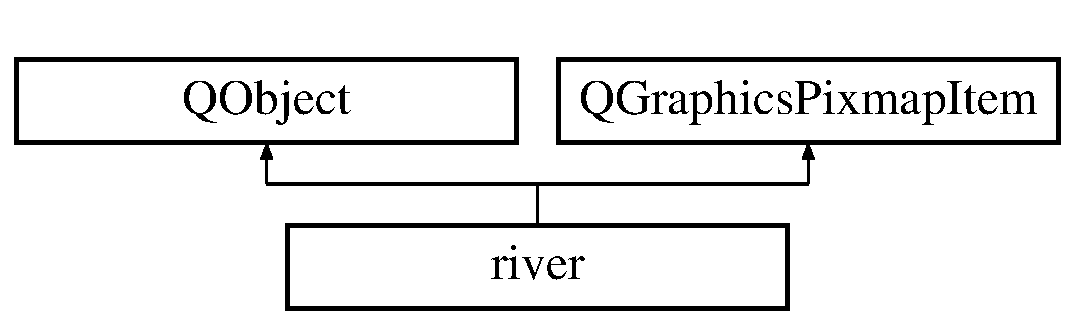
\includegraphics[height=2.000000cm]{classriver}
\end{center}
\end{figure}
\subsection*{Public Member Functions}
\begin{DoxyCompactItemize}
\item 
\hypertarget{classriver_a960a997e38e4de2984933b59b5f54a41}{\hyperlink{classriver_a960a997e38e4de2984933b59b5f54a41}{river} (Q\-Object $\ast$parent=nullptr)}\label{classriver_a960a997e38e4de2984933b59b5f54a41}

\begin{DoxyCompactList}\small\item\em Setting the river's Image. \end{DoxyCompactList}\end{DoxyCompactItemize}


The documentation for this class was generated from the following files\-:\begin{DoxyCompactItemize}
\item 
\hyperlink{river_8h}{river.\-h}\item 
\hyperlink{river_8cpp}{river.\-cpp}\end{DoxyCompactItemize}

\hypertarget{classriverObstacle}{\section{river\-Obstacle Class Reference}
\label{classriverObstacle}\index{river\-Obstacle@{river\-Obstacle}}
}
Inheritance diagram for river\-Obstacle\-:\begin{figure}[H]
\begin{center}
\leavevmode
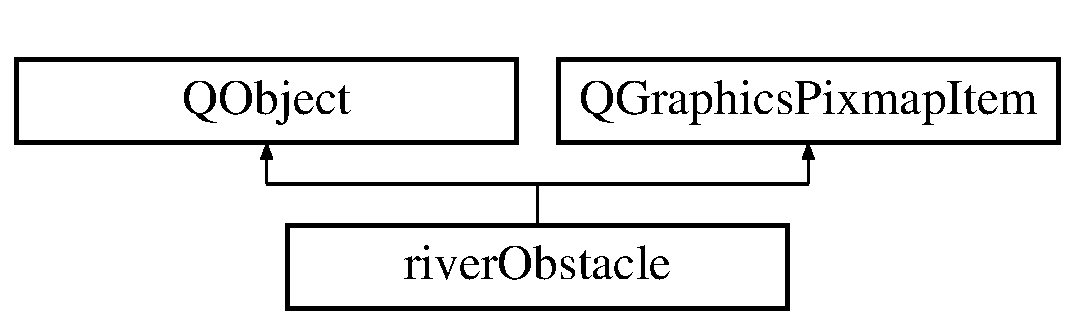
\includegraphics[height=2.000000cm]{classriverObstacle}
\end{center}
\end{figure}
\subsection*{Public Member Functions}
\begin{DoxyCompactItemize}
\item 
\hypertarget{classriverObstacle_ae2f932cd576cd8297809d0ed8d494867}{\hyperlink{classriverObstacle_ae2f932cd576cd8297809d0ed8d494867}{river\-Obstacle} (Q\-Object $\ast$parent=nullptr)}\label{classriverObstacle_ae2f932cd576cd8297809d0ed8d494867}

\begin{DoxyCompactList}\small\item\em Setting the river obstacle's Image. \end{DoxyCompactList}\end{DoxyCompactItemize}


The documentation for this class was generated from the following files\-:\begin{DoxyCompactItemize}
\item 
\hyperlink{riverobstacle_8h}{riverobstacle.\-h}\item 
\hyperlink{riverobstacle_8cpp}{riverobstacle.\-cpp}\end{DoxyCompactItemize}

\hypertarget{classrock}{\section{rock Class Reference}
\label{classrock}\index{rock@{rock}}
}
Inheritance diagram for rock\-:\begin{figure}[H]
\begin{center}
\leavevmode
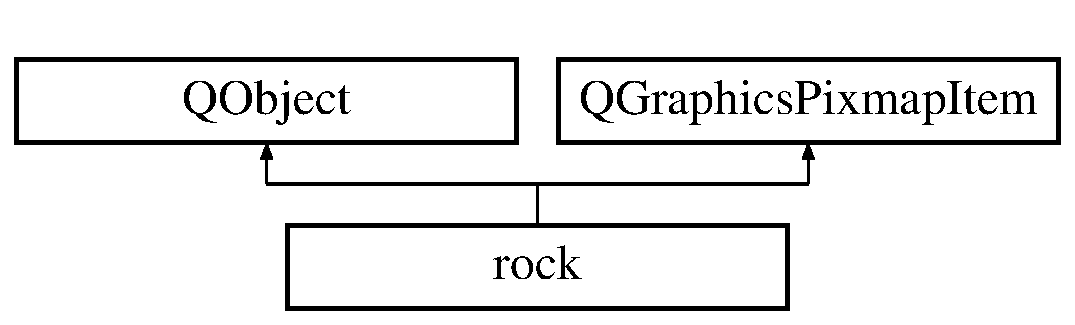
\includegraphics[height=2.000000cm]{classrock}
\end{center}
\end{figure}
\subsection*{Public Member Functions}
\begin{DoxyCompactItemize}
\item 
\hypertarget{classrock_a023e10ff3627f233473609340b1d4f46}{\hyperlink{classrock_a023e10ff3627f233473609340b1d4f46}{rock} (Q\-Object $\ast$parent=nullptr)}\label{classrock_a023e10ff3627f233473609340b1d4f46}

\begin{DoxyCompactList}\small\item\em Setting the rock's Image. \end{DoxyCompactList}\end{DoxyCompactItemize}


The documentation for this class was generated from the following files\-:\begin{DoxyCompactItemize}
\item 
\hyperlink{rock_8h}{rock.\-h}\item 
\hyperlink{rock_8cpp}{rock.\-cpp}\end{DoxyCompactItemize}

\hypertarget{classShield}{\section{Shield Class Reference}
\label{classShield}\index{Shield@{Shield}}
}
Inheritance diagram for Shield\-:\begin{figure}[H]
\begin{center}
\leavevmode
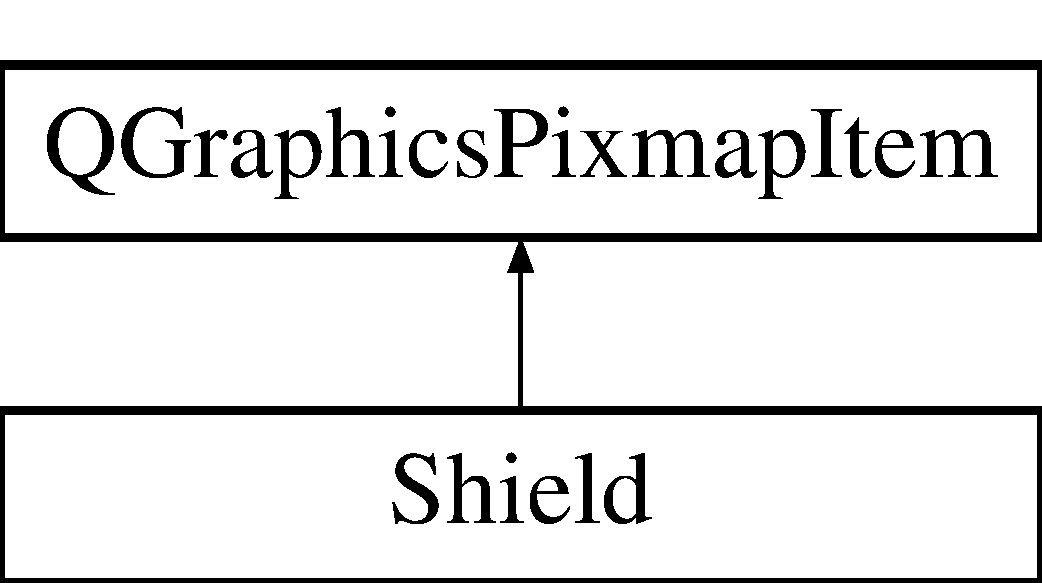
\includegraphics[height=2.000000cm]{classShield}
\end{center}
\end{figure}
\subsection*{Public Member Functions}
\begin{DoxyCompactItemize}
\item 
\hypertarget{classShield_a8a6e827c94750d8c1a1d523cb1b105de}{\hyperlink{classShield_a8a6e827c94750d8c1a1d523cb1b105de}{Shield} ()}\label{classShield_a8a6e827c94750d8c1a1d523cb1b105de}

\begin{DoxyCompactList}\small\item\em Constructor. \end{DoxyCompactList}\end{DoxyCompactItemize}
\subsection*{Public Attributes}
\begin{DoxyCompactItemize}
\item 
\hypertarget{classShield_af36ad92a06058965a4bdc6c21559983b}{Q\-Pixmap $\ast$ \hyperlink{classShield_af36ad92a06058965a4bdc6c21559983b}{icon}}\label{classShield_af36ad92a06058965a4bdc6c21559983b}

\begin{DoxyCompactList}\small\item\em Pixmap holding the image of the shield. \end{DoxyCompactList}\end{DoxyCompactItemize}


The documentation for this class was generated from the following files\-:\begin{DoxyCompactItemize}
\item 
\hyperlink{shield_8h}{shield.\-h}\item 
\hyperlink{shield_8cpp}{shield.\-cpp}\end{DoxyCompactItemize}

\hypertarget{classsignInWidget}{\section{sign\-In\-Widget Class Reference}
\label{classsignInWidget}\index{sign\-In\-Widget@{sign\-In\-Widget}}
}
Inheritance diagram for sign\-In\-Widget\-:\begin{figure}[H]
\begin{center}
\leavevmode
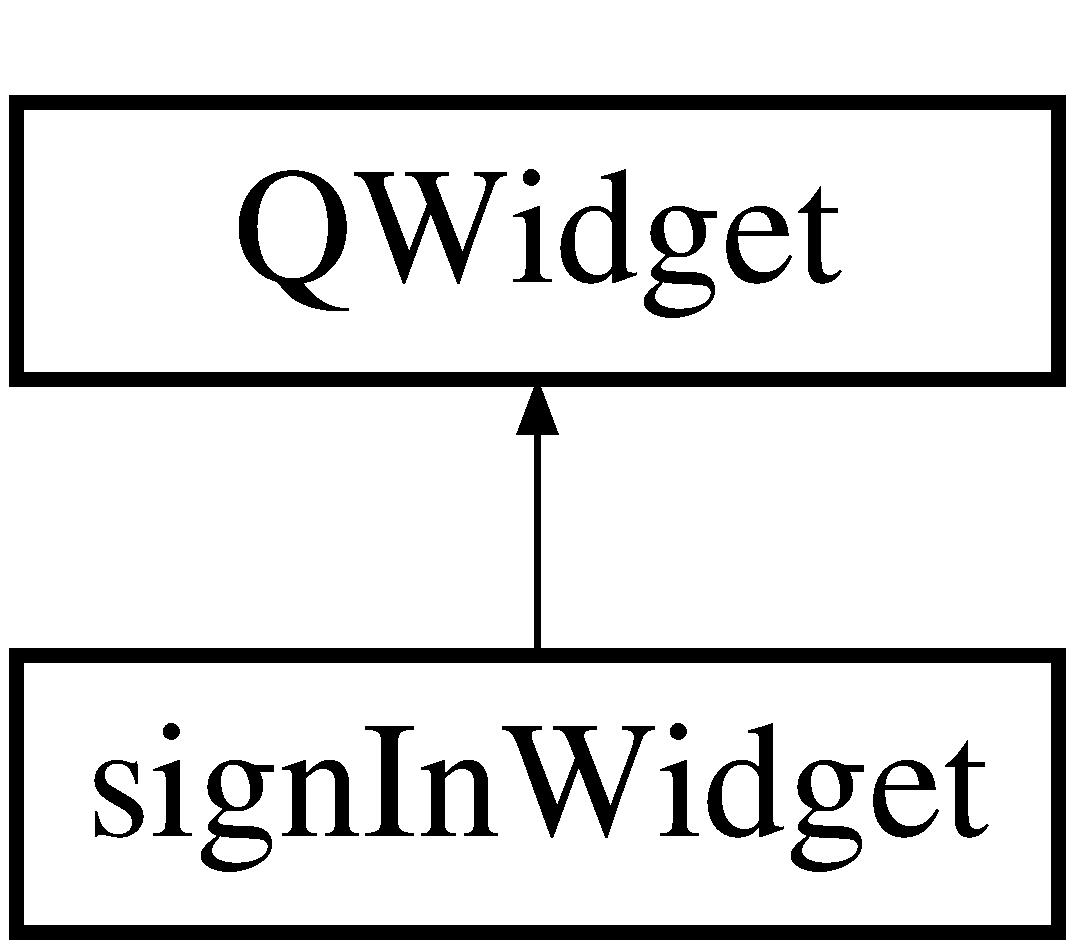
\includegraphics[height=2.000000cm]{classsignInWidget}
\end{center}
\end{figure}
\subsection*{Public Slots}
\begin{DoxyCompactItemize}
\item 
\hypertarget{classsignInWidget_a9baeda329f3f0de1a3b0daeba0829b7d}{void {\bfseries logged\-In} ()}\label{classsignInWidget_a9baeda329f3f0de1a3b0daeba0829b7d}

\item 
\hypertarget{classsignInWidget_aad9c43bc9d4305b6739e7abc8f5e7e51}{void {\bfseries homepage} ()}\label{classsignInWidget_aad9c43bc9d4305b6739e7abc8f5e7e51}

\end{DoxyCompactItemize}
\subsection*{Public Member Functions}
\begin{DoxyCompactItemize}
\item 
\hypertarget{classsignInWidget_a8af614959c9469bc1782a94a955239be}{{\bfseries sign\-In\-Widget} (Q\-Widget $\ast$parent=nullptr)}\label{classsignInWidget_a8af614959c9469bc1782a94a955239be}

\item 
\hypertarget{classsignInWidget_af93991c2a177e15727b97819e94cec30}{void {\bfseries set\-Vertical\-Layout} ()}\label{classsignInWidget_af93991c2a177e15727b97819e94cec30}

\item 
\hypertarget{classsignInWidget_af5fe3a0f9d409a8dcef869812944786c}{void {\bfseries set\-Grid\-Layout} ()}\label{classsignInWidget_af5fe3a0f9d409a8dcef869812944786c}

\end{DoxyCompactItemize}
\subsection*{Public Attributes}
\begin{DoxyCompactItemize}
\item 
\hypertarget{classsignInWidget_ae4ab0ed7451d4bbfe61d8328e83e3766}{Q\-Label $\ast$ {\bfseries user\-Name}}\label{classsignInWidget_ae4ab0ed7451d4bbfe61d8328e83e3766}

\item 
\hypertarget{classsignInWidget_aa753e14dd5bbffccd53966d4d1633e91}{Q\-Label $\ast$ {\bfseries password}}\label{classsignInWidget_aa753e14dd5bbffccd53966d4d1633e91}

\item 
\hypertarget{classsignInWidget_a7632081071e38d207e33a209f8788680}{Q\-Label $\ast$ {\bfseries sign\-In}}\label{classsignInWidget_a7632081071e38d207e33a209f8788680}

\item 
\hypertarget{classsignInWidget_afc7125ac8e5cc70b86e35b14f8da530c}{Q\-Line\-Edit $\ast$ {\bfseries Luser\-Name}}\label{classsignInWidget_afc7125ac8e5cc70b86e35b14f8da530c}

\item 
\hypertarget{classsignInWidget_ac67d104f98b8d0a287ad1e0706df390b}{Q\-Line\-Edit $\ast$ {\bfseries Lpassword}}\label{classsignInWidget_ac67d104f98b8d0a287ad1e0706df390b}

\item 
\hypertarget{classsignInWidget_acb6ab5b841a66c8a29a110f701f07280}{Q\-Push\-Button $\ast$ {\bfseries submit}}\label{classsignInWidget_acb6ab5b841a66c8a29a110f701f07280}

\item 
\hypertarget{classsignInWidget_a17d9ba4c4b39786aaf8f647490479bd1}{Q\-Push\-Button $\ast$ {\bfseries back}}\label{classsignInWidget_a17d9ba4c4b39786aaf8f647490479bd1}

\item 
\hypertarget{classsignInWidget_af8d41288ebb746bba83745a0f69c2317}{const Q\-String {\bfseries esc} =\char`\"{}7727\char`\"{}}\label{classsignInWidget_af8d41288ebb746bba83745a0f69c2317}

\item 
\hypertarget{classsignInWidget_a8f856df0c75d4cc339def8fc414c5f02}{Q\-V\-Box\-Layout $\ast$ {\bfseries Vertical\-L}}\label{classsignInWidget_a8f856df0c75d4cc339def8fc414c5f02}

\item 
\hypertarget{classsignInWidget_ab1633e2a3f7faa14b294122f91468792}{Q\-Grid\-Layout $\ast$ {\bfseries Grid\-L}}\label{classsignInWidget_ab1633e2a3f7faa14b294122f91468792}

\end{DoxyCompactItemize}


The documentation for this class was generated from the following files\-:\begin{DoxyCompactItemize}
\item 
\hyperlink{signinwidget_8h}{signinwidget.\-h}\item 
signinwidget.\-cpp\end{DoxyCompactItemize}

\hypertarget{classSignUpWidget}{\section{Sign\-Up\-Widget Class Reference}
\label{classSignUpWidget}\index{Sign\-Up\-Widget@{Sign\-Up\-Widget}}
}
Inheritance diagram for Sign\-Up\-Widget\-:\begin{figure}[H]
\begin{center}
\leavevmode
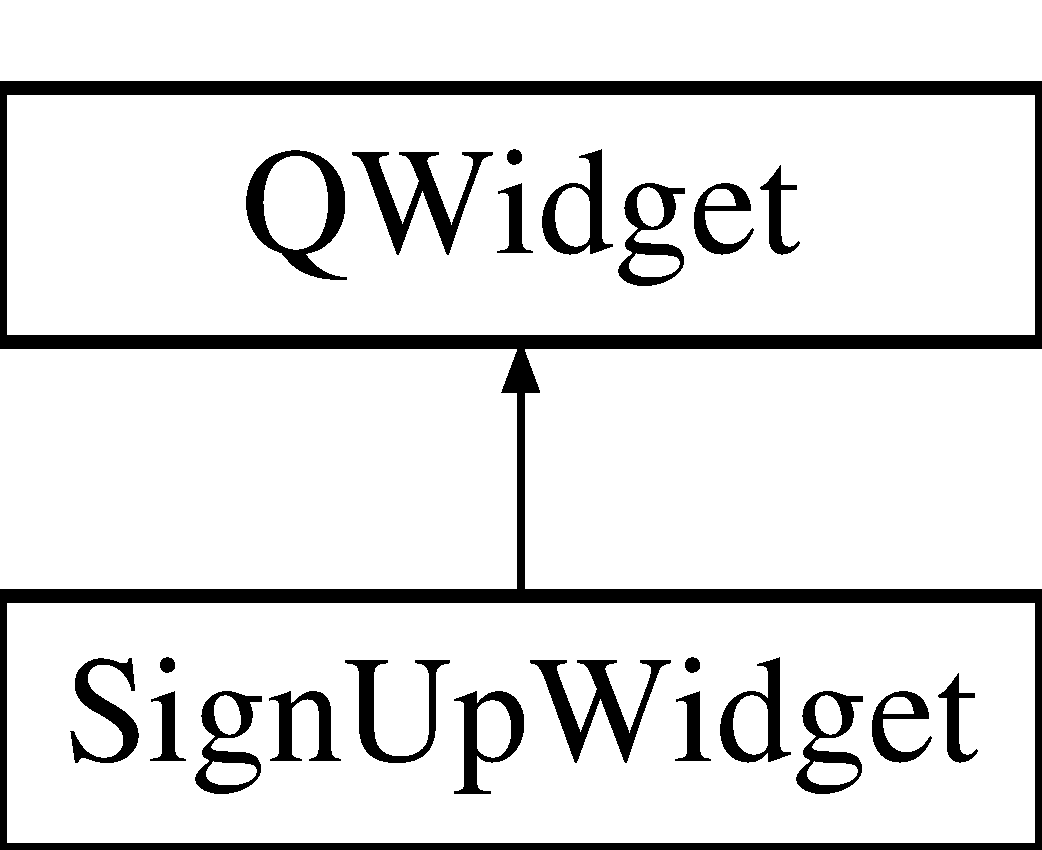
\includegraphics[height=2.000000cm]{classSignUpWidget}
\end{center}
\end{figure}
\subsection*{Public Slots}
\begin{DoxyCompactItemize}
\item 
\hypertarget{classSignUpWidget_abd2b2b0b1b915e3660aa06bf39ee35ab}{void {\bfseries Verify\-Submit\-Slot} ()}\label{classSignUpWidget_abd2b2b0b1b915e3660aa06bf39ee35ab}

\item 
\hypertarget{classSignUpWidget_aadadacbeaa56392604ba4433140568b3}{void {\bfseries Go\-Back\-To\-Log\-On\-Slot} ()}\label{classSignUpWidget_aadadacbeaa56392604ba4433140568b3}

\item 
\hypertarget{classSignUpWidget_a0d4727d741c170dd1f414195d92161a8}{void {\bfseries homepage} ()}\label{classSignUpWidget_a0d4727d741c170dd1f414195d92161a8}

\end{DoxyCompactItemize}
\subsection*{Public Member Functions}
\begin{DoxyCompactItemize}
\item 
\hypertarget{classSignUpWidget_aa6ee3a3bcdfe86cc64a340ffdcc64088}{{\bfseries Sign\-Up\-Widget} (Q\-Widget $\ast$parent=nullptr)}\label{classSignUpWidget_aa6ee3a3bcdfe86cc64a340ffdcc64088}

\end{DoxyCompactItemize}
\subsection*{Public Attributes}
\begin{DoxyCompactItemize}
\item 
\hypertarget{classSignUpWidget_adf986b6b437a72c4e9260d67cb4205d0}{Q\-Label $\ast$ {\bfseries First\-Name}}\label{classSignUpWidget_adf986b6b437a72c4e9260d67cb4205d0}

\item 
\hypertarget{classSignUpWidget_afb060b649dafc986e19ee3f31c9ec05c}{Q\-Label $\ast$ {\bfseries Last\-Name}}\label{classSignUpWidget_afb060b649dafc986e19ee3f31c9ec05c}

\item 
\hypertarget{classSignUpWidget_afd5fc347768a1cae9999586fcc9b9262}{Q\-Label $\ast$ {\bfseries User\-Name}}\label{classSignUpWidget_afd5fc347768a1cae9999586fcc9b9262}

\item 
\hypertarget{classSignUpWidget_a2a9e09af1c22bba762a1624bc84bb89e}{Q\-Label $\ast$ {\bfseries Password}}\label{classSignUpWidget_a2a9e09af1c22bba762a1624bc84bb89e}

\item 
\hypertarget{classSignUpWidget_af289a12775f2439d847d9200ba82e8db}{Q\-Label $\ast$ {\bfseries Confirm\-Pass}}\label{classSignUpWidget_af289a12775f2439d847d9200ba82e8db}

\item 
\hypertarget{classSignUpWidget_a0a03d1cb3203e915867b549943193f03}{Q\-Label $\ast$ {\bfseries Profile\-Picture}}\label{classSignUpWidget_a0a03d1cb3203e915867b549943193f03}

\item 
\hypertarget{classSignUpWidget_aa7ce87272227cedb9fdffac00b9e888b}{Q\-Label $\ast$ {\bfseries Gender}}\label{classSignUpWidget_aa7ce87272227cedb9fdffac00b9e888b}

\item 
\hypertarget{classSignUpWidget_a3f8cdf0e7e5ee8b2eac1bb767a4b7a70}{Q\-Line\-Edit $\ast$ {\bfseries First}}\label{classSignUpWidget_a3f8cdf0e7e5ee8b2eac1bb767a4b7a70}

\item 
\hypertarget{classSignUpWidget_a31a05ead0afc6e4a58086c8be6d39fd0}{Q\-Line\-Edit $\ast$ {\bfseries Last}}\label{classSignUpWidget_a31a05ead0afc6e4a58086c8be6d39fd0}

\item 
\hypertarget{classSignUpWidget_a089503830b77e774b289dbdbe427dec7}{Q\-Line\-Edit $\ast$ {\bfseries User}}\label{classSignUpWidget_a089503830b77e774b289dbdbe427dec7}

\item 
\hypertarget{classSignUpWidget_a935e31891e2dec0532c6225feea3e562}{Q\-Line\-Edit $\ast$ {\bfseries Pass}}\label{classSignUpWidget_a935e31891e2dec0532c6225feea3e562}

\item 
\hypertarget{classSignUpWidget_a3a95b944f5cdd6550b7187a7c90a0d57}{Q\-Line\-Edit $\ast$ {\bfseries Confirm}}\label{classSignUpWidget_a3a95b944f5cdd6550b7187a7c90a0d57}

\item 
\hypertarget{classSignUpWidget_ac4dc8ce992d2730ac8d58cfc45cc2c7f}{Q\-Push\-Button $\ast$ {\bfseries Submit}}\label{classSignUpWidget_ac4dc8ce992d2730ac8d58cfc45cc2c7f}

\item 
\hypertarget{classSignUpWidget_a3003132c3722ebb056bf1332e474e92f}{Q\-Push\-Button $\ast$ {\bfseries back}}\label{classSignUpWidget_a3003132c3722ebb056bf1332e474e92f}

\item 
\hypertarget{classSignUpWidget_a7578b6c691e3f7b1ed4d6c3bb4f99b3c}{Q\-Radio\-Button $\ast$ {\bfseries Male}}\label{classSignUpWidget_a7578b6c691e3f7b1ed4d6c3bb4f99b3c}

\item 
\hypertarget{classSignUpWidget_a356eb348eaf6b373ad9f66041892c85e}{Q\-Radio\-Button $\ast$ {\bfseries Female}}\label{classSignUpWidget_a356eb348eaf6b373ad9f66041892c85e}

\item 
\hypertarget{classSignUpWidget_a747089b24ec2048bf525ffad4edcd4e9}{Q\-Radio\-Button $\ast$ {\bfseries Profile\-Pic1}}\label{classSignUpWidget_a747089b24ec2048bf525ffad4edcd4e9}

\item 
\hypertarget{classSignUpWidget_a9d5a1bf184a799e49112723e3fc310c3}{Q\-Radio\-Button $\ast$ {\bfseries Profile\-Pic2}}\label{classSignUpWidget_a9d5a1bf184a799e49112723e3fc310c3}

\item 
\hypertarget{classSignUpWidget_add7ce942f2f980bfc7fcfd6d0eac50a9}{Q\-Radio\-Button $\ast$ {\bfseries Profile\-Pic3}}\label{classSignUpWidget_add7ce942f2f980bfc7fcfd6d0eac50a9}

\item 
\hypertarget{classSignUpWidget_a47f2fe8025d78c0e9b52e2579aa10cfd}{Q\-Radio\-Button $\ast$ {\bfseries Profile\-Pic4}}\label{classSignUpWidget_a47f2fe8025d78c0e9b52e2579aa10cfd}

\item 
\hypertarget{classSignUpWidget_a4fe807a61e34137d84dd709ef3af434c}{Q\-Group\-Box $\ast$ {\bfseries group\-Box}}\label{classSignUpWidget_a4fe807a61e34137d84dd709ef3af434c}

\item 
\hypertarget{classSignUpWidget_a8cbab0787f691e50dad611971126eae0}{Q\-Grid\-Layout $\ast$ {\bfseries Grid\-Layout}}\label{classSignUpWidget_a8cbab0787f691e50dad611971126eae0}

\item 
\hypertarget{classSignUpWidget_ad88330f83eea902c6334a9a668cae698}{Q\-V\-Box\-Layout $\ast$ {\bfseries Vertical\-Layout}}\label{classSignUpWidget_ad88330f83eea902c6334a9a668cae698}

\item 
\hypertarget{classSignUpWidget_a565b3333be79f3851fdbbb03a59b6cdb}{Q\-Group\-Box $\ast$ {\bfseries preview\-Group\-Box}}\label{classSignUpWidget_a565b3333be79f3851fdbbb03a59b6cdb}

\item 
\hypertarget{classSignUpWidget_a809720773e0d5d303e0773f8626d1e1a}{Q\-Grid\-Layout $\ast$ {\bfseries preview\-Layout}}\label{classSignUpWidget_a809720773e0d5d303e0773f8626d1e1a}

\item 
\hypertarget{classSignUpWidget_a8284b30d58c68e442cbdbf814ef466e4}{Q\-Calendar\-Widget $\ast$ {\bfseries calendar}}\label{classSignUpWidget_a8284b30d58c68e442cbdbf814ef466e4}

\item 
\hypertarget{classSignUpWidget_a231bc2480defd545864f3330d0096127}{const Q\-String {\bfseries esc} =\char`\"{}7727\char`\"{}}\label{classSignUpWidget_a231bc2480defd545864f3330d0096127}

\end{DoxyCompactItemize}


The documentation for this class was generated from the following files\-:\begin{DoxyCompactItemize}
\item 
\hyperlink{signupwidget_8h}{signupwidget.\-h}\item 
signupwidget.\-cpp\end{DoxyCompactItemize}

\hypertarget{classsmallRiver}{\section{small\-River Class Reference}
\label{classsmallRiver}\index{small\-River@{small\-River}}
}
Inheritance diagram for small\-River\-:\begin{figure}[H]
\begin{center}
\leavevmode
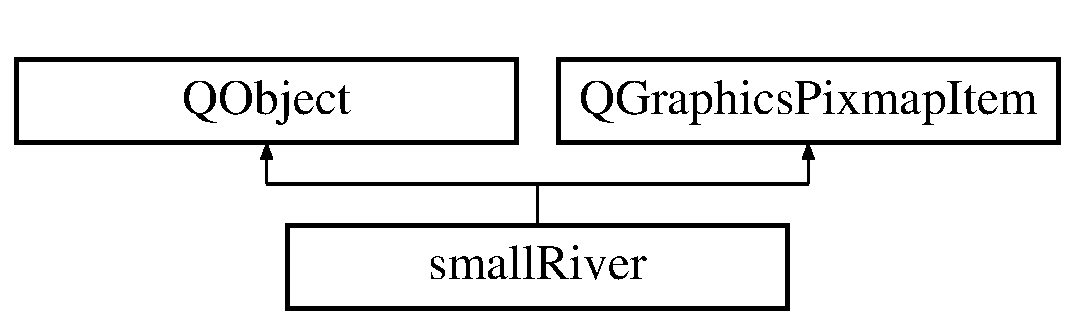
\includegraphics[height=2.000000cm]{classsmallRiver}
\end{center}
\end{figure}
\subsection*{Public Member Functions}
\begin{DoxyCompactItemize}
\item 
\hypertarget{classsmallRiver_ac7dfbda2dce90b878b6b1d7289b6fd5b}{\hyperlink{classsmallRiver_ac7dfbda2dce90b878b6b1d7289b6fd5b}{small\-River} (Q\-Object $\ast$parent=nullptr)}\label{classsmallRiver_ac7dfbda2dce90b878b6b1d7289b6fd5b}

\begin{DoxyCompactList}\small\item\em Setting the small river's Image. \end{DoxyCompactList}\end{DoxyCompactItemize}


The documentation for this class was generated from the following files\-:\begin{DoxyCompactItemize}
\item 
\hyperlink{smallriver_8h}{smallriver.\-h}\item 
\hyperlink{smallriver_8cpp}{smallriver.\-cpp}\end{DoxyCompactItemize}

\hypertarget{classspinach}{\section{spinach Class Reference}
\label{classspinach}\index{spinach@{spinach}}
}
Inheritance diagram for spinach\-:\begin{figure}[H]
\begin{center}
\leavevmode
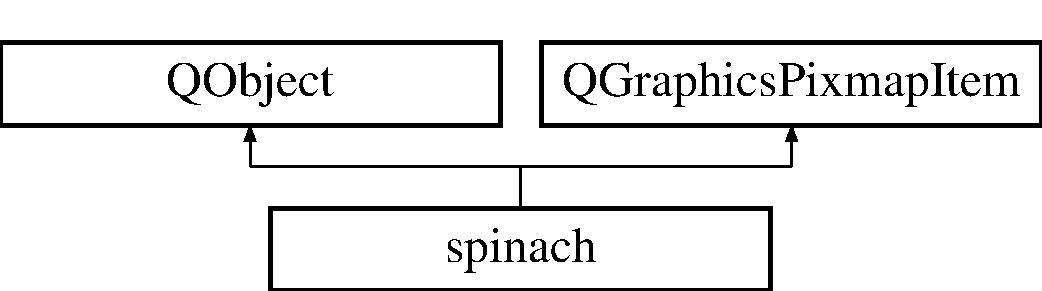
\includegraphics[height=2.000000cm]{classspinach}
\end{center}
\end{figure}
\subsection*{Public Member Functions}
\begin{DoxyCompactItemize}
\item 
\hypertarget{classspinach_aa673f40ede69591ff0e09e2228eafde4}{\hyperlink{classspinach_aa673f40ede69591ff0e09e2228eafde4}{spinach} (Q\-Object $\ast$parent=nullptr)}\label{classspinach_aa673f40ede69591ff0e09e2228eafde4}

\begin{DoxyCompactList}\small\item\em Setting the spinach can's Image. \end{DoxyCompactList}\end{DoxyCompactItemize}


The documentation for this class was generated from the following files\-:\begin{DoxyCompactItemize}
\item 
\hyperlink{spinach_8h}{spinach.\-h}\item 
\hyperlink{spinach_8cpp}{spinach.\-cpp}\end{DoxyCompactItemize}

\hypertarget{classTester}{\section{Tester Class Reference}
\label{classTester}\index{Tester@{Tester}}
}
Inheritance diagram for Tester\-:\begin{figure}[H]
\begin{center}
\leavevmode
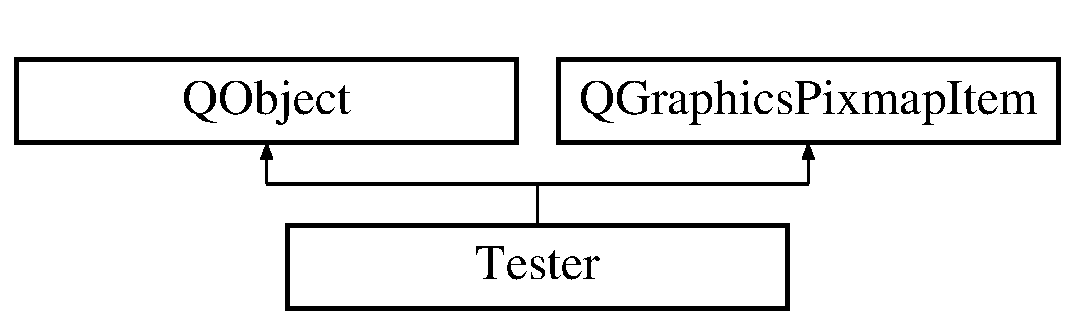
\includegraphics[height=2.000000cm]{classTester}
\end{center}
\end{figure}
\subsection*{Public Member Functions}
\begin{DoxyCompactItemize}
\item 
\hypertarget{classTester_afb0aa17f262b935a12fd05ad3e251164}{{\bfseries Tester} (int, int)}\label{classTester_afb0aa17f262b935a12fd05ad3e251164}

\item 
\hypertarget{classTester_a28def7e2c183306398147efbdd2c4065}{void {\bfseries decrement\-Lives} ()}\label{classTester_a28def7e2c183306398147efbdd2c4065}

\item 
\hypertarget{classTester_a1b36883ccf998c0f71f639483c9bb5ff}{void {\bfseries lose\-Life} ()}\label{classTester_a1b36883ccf998c0f71f639483c9bb5ff}

\item 
\hypertarget{classTester_aac5a0da7cac293ec43ac668f51731d96}{void {\bfseries drink\-Coffee} ()}\label{classTester_aac5a0da7cac293ec43ac668f51731d96}

\item 
\hypertarget{classTester_a6a66686d4d4c4598a327c408ba090dd9}{void {\bfseries show\-Stats} ()}\label{classTester_a6a66686d4d4c4598a327c408ba090dd9}

\end{DoxyCompactItemize}
\subsection*{Public Attributes}
\begin{DoxyCompactItemize}
\item 
\hypertarget{classTester_a893d45f8f768403c93e0892668744cf1}{Q\-Pixmap $\ast$ {\bfseries icon}}\label{classTester_a893d45f8f768403c93e0892668744cf1}

\item 
\hypertarget{classTester_ad1d75f921be24ad1c4ca52250f631655}{Q\-Timer $\ast$ {\bfseries timer}}\label{classTester_ad1d75f921be24ad1c4ca52250f631655}

\item 
\hypertarget{classTester_a59495affb31a5fa5daa0fe96ef5bfa28}{int {\bfseries lives}}\label{classTester_a59495affb31a5fa5daa0fe96ef5bfa28}

\item 
\hypertarget{classTester_af42e09fb691bbbf3ba2fd0826e2c84bd}{int {\bfseries souls}}\label{classTester_af42e09fb691bbbf3ba2fd0826e2c84bd}

\item 
\hypertarget{classTester_af967debae52b5edefbd81b8c6feab26b}{int {\bfseries starting\-X}}\label{classTester_af967debae52b5edefbd81b8c6feab26b}

\item 
\hypertarget{classTester_a56259a760a37339190abe1d41f4a270c}{int {\bfseries starting\-Y}}\label{classTester_a56259a760a37339190abe1d41f4a270c}

\end{DoxyCompactItemize}


The documentation for this class was generated from the following files\-:\begin{DoxyCompactItemize}
\item 
\hyperlink{tester_8h}{tester.\-h}\item 
\hyperlink{tester_8cpp}{tester.\-cpp}\end{DoxyCompactItemize}

\hypertarget{classTestingIcon}{\section{Testing\-Icon Class Reference}
\label{classTestingIcon}\index{Testing\-Icon@{Testing\-Icon}}
}
Inheritance diagram for Testing\-Icon\-:\begin{figure}[H]
\begin{center}
\leavevmode
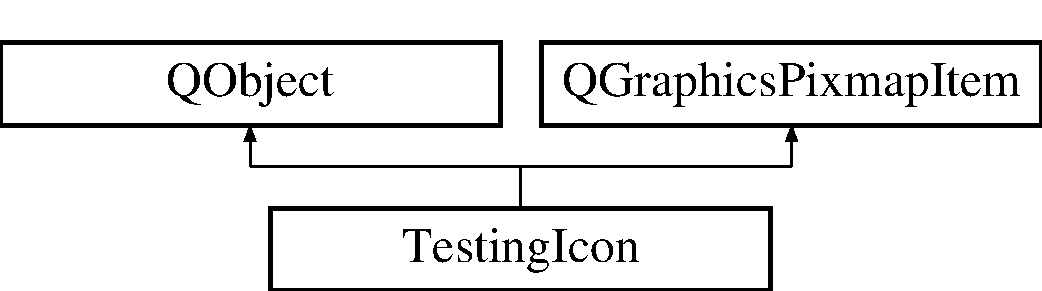
\includegraphics[height=2.000000cm]{classTestingIcon}
\end{center}
\end{figure}
\subsection*{Public Slots}
\begin{DoxyCompactItemize}
\item 
\hypertarget{classTestingIcon_a075c1421405dfeca57ce328f5fa6bd04}{void {\bfseries re\-Activate} ()}\label{classTestingIcon_a075c1421405dfeca57ce328f5fa6bd04}

\end{DoxyCompactItemize}
\subsection*{Public Member Functions}
\begin{DoxyCompactItemize}
\item 
\hypertarget{classTestingIcon_a2c069d959088b157cbcdf4d60656f426}{void {\bfseries de\-Activate} ()}\label{classTestingIcon_a2c069d959088b157cbcdf4d60656f426}

\end{DoxyCompactItemize}
\subsection*{Public Attributes}
\begin{DoxyCompactItemize}
\item 
\hypertarget{classTestingIcon_ae78a033bb145ea88596d504a8ef32d4b}{Q\-Pixmap $\ast$ {\bfseries icon}}\label{classTestingIcon_ae78a033bb145ea88596d504a8ef32d4b}

\item 
\hypertarget{classTestingIcon_a9391584daf10f909a82dd428e6641281}{bool {\bfseries is\-Hidden}}\label{classTestingIcon_a9391584daf10f909a82dd428e6641281}

\item 
\hypertarget{classTestingIcon_a5c8e56116c090b6867ca7c548e841366}{Q\-Timer $\ast$ {\bfseries timer}}\label{classTestingIcon_a5c8e56116c090b6867ca7c548e841366}

\end{DoxyCompactItemize}


The documentation for this class was generated from the following files\-:\begin{DoxyCompactItemize}
\item 
\hyperlink{testingicon_8h}{testingicon.\-h}\item 
\hyperlink{testingicon_8cpp}{testingicon.\-cpp}\end{DoxyCompactItemize}

\hypertarget{classWall}{\section{Wall Class Reference}
\label{classWall}\index{Wall@{Wall}}
}
Inheritance diagram for Wall\-:\begin{figure}[H]
\begin{center}
\leavevmode
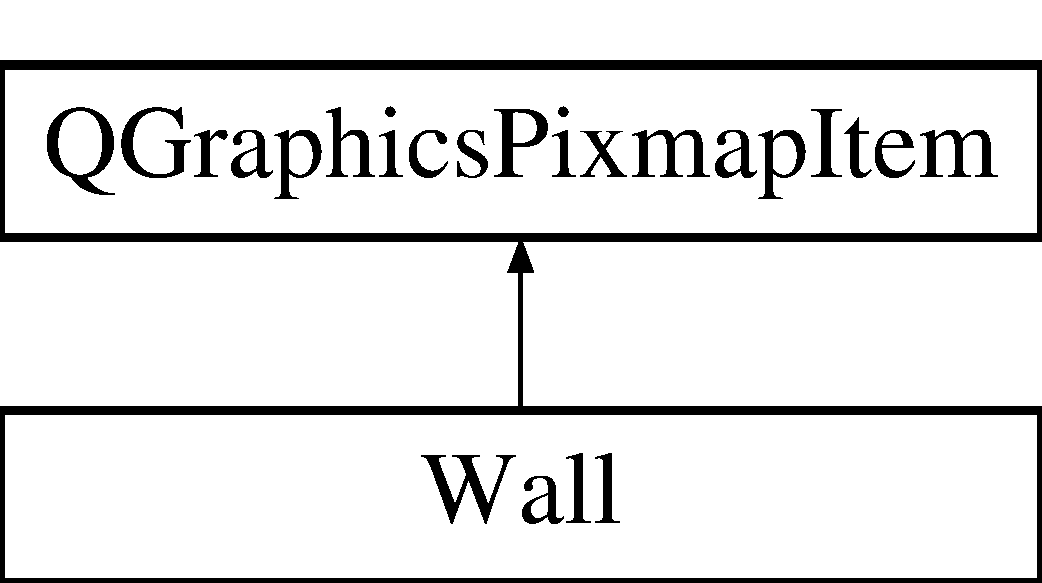
\includegraphics[height=2.000000cm]{classWall}
\end{center}
\end{figure}
\subsection*{Public Attributes}
\begin{DoxyCompactItemize}
\item 
\hypertarget{classWall_a815f7b9b4b8d1c3c8747978830572bc0}{Q\-Pixmap $\ast$ {\bfseries icon}}\label{classWall_a815f7b9b4b8d1c3c8747978830572bc0}

\end{DoxyCompactItemize}


The documentation for this class was generated from the following files\-:\begin{DoxyCompactItemize}
\item 
wall.\-h\item 
wall.\-cpp\end{DoxyCompactItemize}

\hypertarget{classWon}{\section{Won Class Reference}
\label{classWon}\index{Won@{Won}}
}
Inheritance diagram for Won\-:\begin{figure}[H]
\begin{center}
\leavevmode
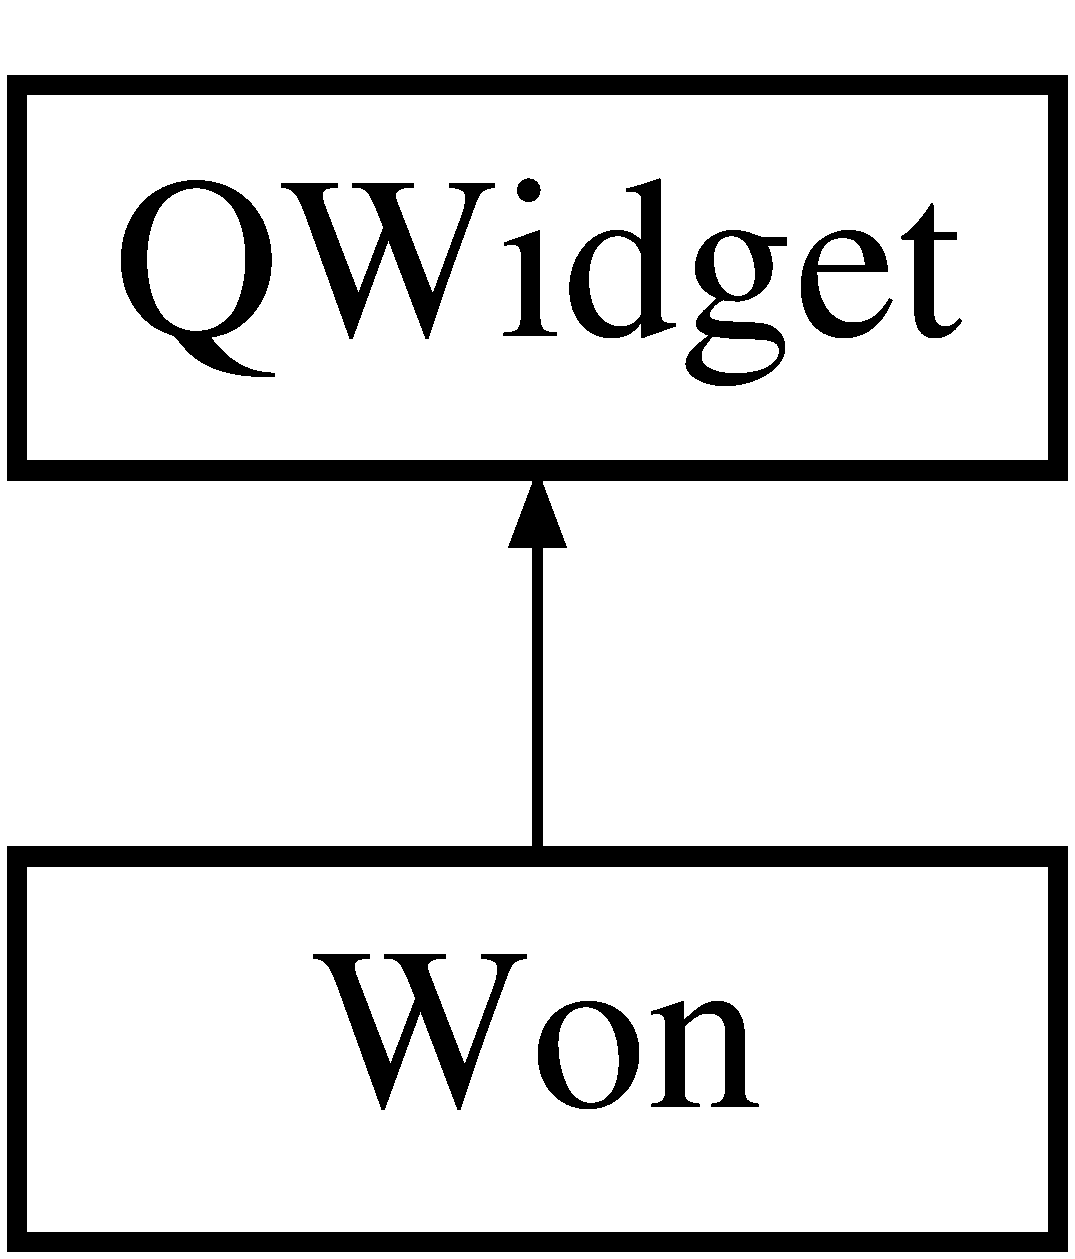
\includegraphics[height=2.000000cm]{classWon}
\end{center}
\end{figure}
\subsection*{Public Member Functions}
\begin{DoxyCompactItemize}
\item 
\hypertarget{classWon_ac5dce31ed2c2d4a9c2f14443e9cd3ca9}{\hyperlink{classWon_ac5dce31ed2c2d4a9c2f14443e9cd3ca9}{Won} (Q\-Widget $\ast$parent)}\label{classWon_ac5dce31ed2c2d4a9c2f14443e9cd3ca9}

\begin{DoxyCompactList}\small\item\em Setting the win pop up window content. \end{DoxyCompactList}\item 
\hyperlink{classWon_ad1d2faac43a1e445889e6d1f9de1ed1d}{Won} (int, int)
\end{DoxyCompactItemize}


\subsection{Constructor \& Destructor Documentation}
\hypertarget{classWon_ad1d2faac43a1e445889e6d1f9de1ed1d}{\index{Won@{Won}!Won@{Won}}
\index{Won@{Won}!Won@{Won}}
\subsubsection[{Won}]{\setlength{\rightskip}{0pt plus 5cm}Won\-::\-Won (
\begin{DoxyParamCaption}
\item[{int}]{level, }
\item[{int}]{lives}
\end{DoxyParamCaption}
)}}\label{classWon_ad1d2faac43a1e445889e6d1f9de1ed1d}
$<$If level is 8 and user won therefore he would have the entire game. 

The documentation for this class was generated from the following files\-:\begin{DoxyCompactItemize}
\item 
\hyperlink{won_8h}{won.\-h}\item 
\hyperlink{won_8cpp}{won.\-cpp}\end{DoxyCompactItemize}

\chapter{File Documentation}
\hypertarget{boat_8cpp}{\section{boat.\-cpp File Reference}
\label{boat_8cpp}\index{boat.\-cpp@{boat.\-cpp}}
}


Contains \hyperlink{classPopeye}{Popeye} class definition.  


{\ttfamily \#include \char`\"{}boat.\-h\char`\"{}}\\*


\subsection{Detailed Description}
Contains \hyperlink{classPopeye}{Popeye} class definition. \begin{DoxyAuthor}{Author}
Camille Farhat \& Ali Haidoura 
\end{DoxyAuthor}

\hypertarget{boat_8h}{\section{boat.\-h File Reference}
\label{boat_8h}\index{boat.\-h@{boat.\-h}}
}


contains boat class definition  


{\ttfamily \#include $<$Q\-Object$>$}\\*
{\ttfamily \#include $<$Q\-Graphics\-Pixmap\-Item$>$}\\*
\subsection*{Classes}
\begin{DoxyCompactItemize}
\item 
class \hyperlink{classboat}{boat}
\end{DoxyCompactItemize}


\subsection{Detailed Description}
contains boat class definition \begin{DoxyAuthor}{Author}
Camille Farhat \& Ali Haidar 
\end{DoxyAuthor}

\hypertarget{bug_8cpp}{\section{bug.\-cpp File Reference}
\label{bug_8cpp}\index{bug.\-cpp@{bug.\-cpp}}
}


contains \hyperlink{classBug}{Bug} class definitions  


{\ttfamily \#include \char`\"{}bug.\-h\char`\"{}}\\*
{\ttfamily \#include \char`\"{}tester.\-h\char`\"{}}\\*
{\ttfamily \#include \char`\"{}minibug.\-h\char`\"{}}\\*
{\ttfamily \#include $<$Q\-Transform$>$}\\*


\subsection{Detailed Description}
contains \hyperlink{classBug}{Bug} class definitions \begin{DoxyAuthor}{Author}
Ali Al Akbar Haidoura 
\end{DoxyAuthor}

\hypertarget{bug_8h}{\section{bug.\-h File Reference}
\label{bug_8h}\index{bug.\-h@{bug.\-h}}
}


Q\-Graphics\-Pixmap\-Item representing the bugs.  


{\ttfamily \#include $<$Q\-Graphics\-Pixmap\-Item$>$}\\*
{\ttfamily \#include $<$Q\-Timer$>$}\\*
\subsection*{Classes}
\begin{DoxyCompactItemize}
\item 
class \hyperlink{classBug}{Bug}
\end{DoxyCompactItemize}


\subsection{Detailed Description}
Q\-Graphics\-Pixmap\-Item representing the bugs. \hyperlink{classBug}{Bug} objects move horizentally, shoot at the player when in sight also contains collision logic

\begin{DoxyAuthor}{Author}
Ali Al Akbar Haidoura 
\end{DoxyAuthor}

\hypertarget{bullet_8cpp}{\section{bullet.\-cpp File Reference}
\label{bullet_8cpp}\index{bullet.\-cpp@{bullet.\-cpp}}
}


contains \hyperlink{classBullet}{Bullet} class definitions  


{\ttfamily \#include \char`\"{}bullet.\-h\char`\"{}}\\*
{\ttfamily \#include \char`\"{}wall.\-h\char`\"{}}\\*
{\ttfamily \#include \char`\"{}bug.\-h\char`\"{}}\\*
{\ttfamily \#include \char`\"{}minibug.\-h\char`\"{}}\\*
{\ttfamily \#include $<$Q\-Transform$>$}\\*


\subsection{Detailed Description}
contains \hyperlink{classBullet}{Bullet} class definitions \begin{DoxyAuthor}{Author}
Ali Al Akbar Haidoura 
\end{DoxyAuthor}

\hypertarget{bullet_8h}{\section{bullet.\-h File Reference}
\label{bullet_8h}\index{bullet.\-h@{bullet.\-h}}
}


Q\-Graphics\-Pixmap\-Item representing the bullets.  


{\ttfamily \#include $<$Q\-Graphics\-Pixmap\-Item$>$}\\*
{\ttfamily \#include $<$Q\-Timer$>$}\\*
{\ttfamily \#include $<$Q\-Debug$>$}\\*
{\ttfamily \#include \char`\"{}game2scene.\-h\char`\"{}}\\*
\subsection*{Classes}
\begin{DoxyCompactItemize}
\item 
class \hyperlink{classBullet}{Bullet}
\end{DoxyCompactItemize}


\subsection{Detailed Description}
Q\-Graphics\-Pixmap\-Item representing the bullets. \begin{DoxyAuthor}{Author}
Ali Al Akbar Haidoura 
\end{DoxyAuthor}

\hypertarget{coffeecup_8cpp}{\section{coffeecup.\-cpp File Reference}
\label{coffeecup_8cpp}\index{coffeecup.\-cpp@{coffeecup.\-cpp}}
}


Contains \hyperlink{classCoffeeCup}{Coffee\-Cup} Class definitions.  


{\ttfamily \#include \char`\"{}coffeecup.\-h\char`\"{}}\\*


\subsection{Detailed Description}
Contains \hyperlink{classCoffeeCup}{Coffee\-Cup} Class definitions. \begin{DoxyAuthor}{Author}
Ali Al Akbar Haidoura 
\end{DoxyAuthor}

\hypertarget{coffeecup_8h}{\section{coffeecup.\-h File Reference}
\label{coffeecup_8h}\index{coffeecup.\-h@{coffeecup.\-h}}
}


Q\-Graphics\-Pixmap\-Item representing the Coffee Cup.  


{\ttfamily \#include $<$Q\-Graphics\-Pixmap\-Item$>$}\\*
\subsection*{Classes}
\begin{DoxyCompactItemize}
\item 
class \hyperlink{classCoffeeCup}{Coffee\-Cup}
\end{DoxyCompactItemize}


\subsection{Detailed Description}
Q\-Graphics\-Pixmap\-Item representing the Coffee Cup. \begin{DoxyAuthor}{Author}
Ali Al Akbar Haidoura 
\end{DoxyAuthor}

\hypertarget{game1scene_8cpp}{\section{game1scene.\-cpp File Reference}
\label{game1scene_8cpp}\index{game1scene.\-cpp@{game1scene.\-cpp}}
}


contains Game1's class definition  


{\ttfamily \#include $<$Q\-Object$>$}\\*
{\ttfamily \#include $<$Q\-Graphics\-Pixmap\-Item$>$}\\*
{\ttfamily \#include $<$Q\-Graphics\-Scene$>$}\\*
{\ttfamily \#include $<$Qt\-Events$>$}\\*
{\ttfamily \#include $<$Q\-Timer$>$}\\*
{\ttfamily \#include \char`\"{}popeye.\-h\char`\"{}}\\*
{\ttfamily \#include \char`\"{}locks.\-h\char`\"{}}\\*
{\ttfamily \#include \char`\"{}game1scene.\-h\char`\"{}}\\*
{\ttfamily \#include \char`\"{}gameswidget.\-h\char`\"{}}\\*
{\ttfamily \#include \char`\"{}gameover.\-h\char`\"{}}\\*


\subsection{Detailed Description}
contains Game1's class definition This is the scene where we see \hyperlink{classPopeye}{Popeye}, Olive and the locks. Each time time popeye passes a level, the corresponding lock is hiden and popeye's position is updated. The let's Go Button is the button that lunches the user to the corresponding level.

\begin{DoxyAuthor}{Author}
Camille Farhat \& Ali Haidoura 
\end{DoxyAuthor}

\hypertarget{game1scene_8h}{\section{game1scene.\-h File Reference}
\label{game1scene_8h}\index{game1scene.\-h@{game1scene.\-h}}
}


The Game's scene.  


{\ttfamily \#include $<$Q\-Object$>$}\\*
{\ttfamily \#include $<$Q\-Graphics\-Scene$>$}\\*
{\ttfamily \#include $<$Q\-Graphics\-Pixmap\-Item$>$}\\*
{\ttfamily \#include $<$Qt\-Events$>$}\\*
{\ttfamily \#include $<$Q\-Timer$>$}\\*
{\ttfamily \#include $<$Qt\-Widgets$>$}\\*
{\ttfamily \#include \char`\"{}popeye.\-h\char`\"{}}\\*
{\ttfamily \#include \char`\"{}locks.\-h\char`\"{}}\\*
{\ttfamily \#include \char`\"{}levelsscene.\-h\char`\"{}}\\*
\subsection*{Classes}
\begin{DoxyCompactItemize}
\item 
class \hyperlink{classgame1scene}{game1scene}
\end{DoxyCompactItemize}


\subsection{Detailed Description}
The Game's scene. This is the header file for our first game's scene. It publicly inherits from Q\-Graphics\-Scene. 
\hypertarget{game2scene_8cpp}{\section{game2scene.\-cpp File Reference}
\label{game2scene_8cpp}\index{game2scene.\-cpp@{game2scene.\-cpp}}
}


Contains \hyperlink{classGame2Scene}{Game2\-Scene} Class definitions.  


{\ttfamily \#include \char`\"{}game2scene.\-h\char`\"{}}\\*
{\ttfamily \#include \char`\"{}levelparser.\-h\char`\"{}}\\*
{\ttfamily \#include \char`\"{}bug.\-h\char`\"{}}\\*
{\ttfamily \#include \char`\"{}wall.\-h\char`\"{}}\\*
{\ttfamily \#include \char`\"{}coffeecup.\-h\char`\"{}}\\*
{\ttfamily \#include \char`\"{}qualitycontrolicon.\-h\char`\"{}}\\*
{\ttfamily \#include \char`\"{}testingicon.\-h\char`\"{}}\\*
{\ttfamily \#include \char`\"{}shield.\-h\char`\"{}}\\*
{\ttfamily \#include \char`\"{}bullet.\-h\char`\"{}}\\*
{\ttfamily \#include $<$Q\-Debug$>$}\\*
{\ttfamily \#include $<$Q\-Graphics\-Item$>$}\\*


\subsection{Detailed Description}
Contains \hyperlink{classGame2Scene}{Game2\-Scene} Class definitions. \begin{DoxyAuthor}{Author}
Ali Al Akbar Haidoura 
\end{DoxyAuthor}

\hypertarget{game2scene_8h}{\section{game2scene.\-h File Reference}
\label{game2scene_8h}\index{game2scene.\-h@{game2scene.\-h}}
}


The scene in which all the logic and items of Game2 are located.  


{\ttfamily \#include $<$Q\-Graphics\-Scene$>$}\\*
{\ttfamily \#include $<$Q\-Graphics\-View$>$}\\*
{\ttfamily \#include $<$Q\-Timer$>$}\\*
{\ttfamily \#include $<$Q\-Label$>$}\\*
{\ttfamily \#include $<$Q\-Push\-Button$>$}\\*
{\ttfamily \#include \char`\"{}tester.\-h\char`\"{}}\\*
{\ttfamily \#include \char`\"{}qualitycontrolicon.\-h\char`\"{}}\\*
{\ttfamily \#include \char`\"{}lifecounter.\-h\char`\"{}}\\*
{\ttfamily \#include \char`\"{}testingicon.\-h\char`\"{}}\\*
{\ttfamily \#include \char`\"{}bug.\-h\char`\"{}}\\*
\subsection*{Classes}
\begin{DoxyCompactItemize}
\item 
class \hyperlink{classGame2Scene}{Game2\-Scene}
\end{DoxyCompactItemize}


\subsection{Detailed Description}
The scene in which all the logic and items of Game2 are located. \begin{DoxyAuthor}{Author}
Ali Al Akbar Haidoura 
\end{DoxyAuthor}

\hypertarget{gameswidget_8cpp}{\section{gameswidget.\-cpp File Reference}
\label{gameswidget_8cpp}\index{gameswidget.\-cpp@{gameswidget.\-cpp}}
}


contains Game1-\/2 Links  


{\ttfamily \#include $<$Qt\-Widgets$>$}\\*
{\ttfamily \#include $<$Q\-Object$>$}\\*
{\ttfamily \#include $<$Q\-Pixmap$>$}\\*
{\ttfamily \#include $<$Q\-Graphics\-Item$>$}\\*
{\ttfamily \#include $<$Q\-Graphics\-Pixmap\-Item$>$}\\*
{\ttfamily \#include $<$Q\-Graphics\-Scene$>$}\\*
{\ttfamily \#include $<$Q\-Graphics\-View$>$}\\*
{\ttfamily \#include $<$Q\-Application$>$}\\*
{\ttfamily \#include $<$Q\-Dir$>$}\\*
{\ttfamily \#include \char`\"{}game1scene.\-h\char`\"{}}\\*
{\ttfamily \#include \char`\"{}gameswidget.\-h\char`\"{}}\\*
{\ttfamily \#include \char`\"{}levelparser.\-h\char`\"{}}\\*


\subsection{Detailed Description}
contains Game1-\/2 Links \begin{DoxyAuthor}{Author}
Camille Farhat \& Ali Haidoura 
\end{DoxyAuthor}

\hypertarget{hints_8cpp}{\section{hints.\-cpp File Reference}
\label{hints_8cpp}\index{hints.\-cpp@{hints.\-cpp}}
}


Shows the appropriate hints in a pop up window.  


{\ttfamily \#include \char`\"{}hints.\-h\char`\"{}}\\*
{\ttfamily \#include \char`\"{}levels.\-h\char`\"{}}\\*
{\ttfamily \#include $<$Q\-Label$>$}\\*
{\ttfamily \#include $<$Q\-V\-Box\-Layout$>$}\\*


\subsection{Detailed Description}
Shows the appropriate hints in a pop up window. \begin{DoxyAuthor}{Author}
Camille Farhat \& Ali Haidoura 
\end{DoxyAuthor}

\hypertarget{hints_8h}{\section{hints.\-h File Reference}
\label{hints_8h}\index{hints.\-h@{hints.\-h}}
}


The Level's scene's Hints.  


{\ttfamily \#include $<$Q\-Widget$>$}\\*
\subsection*{Classes}
\begin{DoxyCompactItemize}
\item 
class \hyperlink{classhints}{hints}
\end{DoxyCompactItemize}


\subsection{Detailed Description}
The Level's scene's Hints. Pop up window that will display the hints. 
\hypertarget{instruction_8cpp}{\section{instruction.\-cpp File Reference}
\label{instruction_8cpp}\index{instruction.\-cpp@{instruction.\-cpp}}
}


Shows the initial instructions to start the game in a pop up window.  


{\ttfamily \#include \char`\"{}instruction.\-h\char`\"{}}\\*
{\ttfamily \#include $<$Q\-Label$>$}\\*
{\ttfamily \#include $<$Q\-Layout$>$}\\*


\subsection{Detailed Description}
Shows the initial instructions to start the game in a pop up window. \begin{DoxyAuthor}{Author}
Camille Farhat \& Ali Haidoura 
\end{DoxyAuthor}

\hypertarget{instruction_8h}{\section{instruction.\-h File Reference}
\label{instruction_8h}\index{instruction.\-h@{instruction.\-h}}
}


The Level's scene's levels pop up used for displaying instructions.  


{\ttfamily \#include $<$Q\-Widget$>$}\\*
\subsection*{Classes}
\begin{DoxyCompactItemize}
\item 
class \hyperlink{classinstruction}{instruction}
\end{DoxyCompactItemize}


\subsection{Detailed Description}
The Level's scene's levels pop up used for displaying instructions. Pop up window that will display the Initial Instructions before starting the Game. 
\hypertarget{levelparser_8cpp}{\section{levelparser.\-cpp File Reference}
\label{levelparser_8cpp}\index{levelparser.\-cpp@{levelparser.\-cpp}}
}


Contains \hyperlink{classLevelParser}{Level\-Parser} Class definitions.  


{\ttfamily \#include \char`\"{}levelparser.\-h\char`\"{}}\\*
{\ttfamily \#include $<$Q\-Debug$>$}\\*
{\ttfamily \#include $<$bug.\-h$>$}\\*
{\ttfamily \#include \char`\"{}wall.\-h\char`\"{}}\\*
{\ttfamily \#include \char`\"{}tester.\-h\char`\"{}}\\*
{\ttfamily \#include \char`\"{}testingicon.\-h\char`\"{}}\\*
{\ttfamily \#include \char`\"{}shield.\-h\char`\"{}}\\*
{\ttfamily \#include \char`\"{}coffeecup.\-h\char`\"{}}\\*
{\ttfamily \#include \char`\"{}qualitycontrolicon.\-h\char`\"{}}\\*


\subsection{Detailed Description}
Contains \hyperlink{classLevelParser}{Level\-Parser} Class definitions. \begin{DoxyAuthor}{Author}
Ali Al Akbar Haidoura 
\end{DoxyAuthor}

\hypertarget{levelparser_8h}{\section{levelparser.\-h File Reference}
\label{levelparser_8h}\index{levelparser.\-h@{levelparser.\-h}}
}


Parses the game2 levels from the text files.  


{\ttfamily \#include $<$Q\-String$>$}\\*
{\ttfamily \#include $<$Q\-Dir$>$}\\*
{\ttfamily \#include \char`\"{}game2scene.\-h\char`\"{}}\\*
\subsection*{Classes}
\begin{DoxyCompactItemize}
\item 
class \hyperlink{classLevelParser}{Level\-Parser}
\end{DoxyCompactItemize}


\subsection{Detailed Description}
Parses the game2 levels from the text files. \begin{DoxyAuthor}{Author}
Ali Al Akbar Haidoura 
\end{DoxyAuthor}

\hypertarget{levels_8cpp}{\section{levels.\-cpp File Reference}
\label{levels_8cpp}\index{levels.\-cpp@{levels.\-cpp}}
}


Setting up the different specs for each level to load them dynamically everytime a user starts a level.  


{\ttfamily \#include \char`\"{}levels.\-h\char`\"{}}\\*


\subsection{Detailed Description}
Setting up the different specs for each level to load them dynamically everytime a user starts a level. \begin{DoxyAuthor}{Author}
Camille Farhat \& Ali Haidoura 
\end{DoxyAuthor}

\hypertarget{levels_8h}{\section{levels.\-h File Reference}
\label{levels_8h}\index{levels.\-h@{levels.\-h}}
}


The Level Object.  


{\ttfamily \#include $<$Q\-Widget$>$}\\*
{\ttfamily \#include $<$Q\-String$>$}\\*
{\ttfamily \#include $<$Q\-Timer$>$}\\*
{\ttfamily \#include $<$Qt\-Widgets$>$}\\*
{\ttfamily \#include $<$Q\-Object$>$}\\*
{\ttfamily \#include \char`\"{}spinach.\-h\char`\"{}}\\*
{\ttfamily \#include \char`\"{}popeye.\-h\char`\"{}}\\*
\subsection*{Classes}
\begin{DoxyCompactItemize}
\item 
class \hyperlink{classlevels}{levels}
\end{DoxyCompactItemize}


\subsection{Detailed Description}
The Level Object. Creating a Level Object that will be passed to every scene to load the respective level. 
\hypertarget{levelsscene_8cpp}{\section{levelsscene.\-cpp File Reference}
\label{levelsscene_8cpp}\index{levelsscene.\-cpp@{levelsscene.\-cpp}}
}


Contains Game1's class definition.  


{\ttfamily \#include \char`\"{}levelsscene.\-h\char`\"{}}\\*
{\ttfamily \#include \char`\"{}levels.\-h\char`\"{}}\\*
{\ttfamily \#include \char`\"{}hints.\-h\char`\"{}}\\*
{\ttfamily \#include \char`\"{}lost.\-h\char`\"{}}\\*
{\ttfamily \#include \char`\"{}won.\-h\char`\"{}}\\*
{\ttfamily \#include \char`\"{}instruction.\-h\char`\"{}}\\*
{\ttfamily \#include \char`\"{}boat.\-h\char`\"{}}\\*


\subsection{Detailed Description}
Contains Game1's class definition. This file is creating the enviorment of our game. Setting everything from background image to the timer, popeye, the spinach cans, the boat and the river obstacles and other level-\/specific specifications. The user will be writing code into the text editor. This code will be chekcked and popeye will move accordingly.

\begin{DoxyAuthor}{Author}
Camille Farhat \& Ali Haidoura 
\end{DoxyAuthor}

\hypertarget{lifecounter_8cpp}{\section{lifecounter.\-cpp File Reference}
\label{lifecounter_8cpp}\index{lifecounter.\-cpp@{lifecounter.\-cpp}}
}


Contains \hyperlink{classLifeCounter}{Life\-Counter} Class definitions.  


{\ttfamily \#include \char`\"{}lifecounter.\-h\char`\"{}}\\*


\subsection{Detailed Description}
Contains \hyperlink{classLifeCounter}{Life\-Counter} Class definitions. \begin{DoxyAuthor}{Author}
Ali Al Akbar Haidoura 
\end{DoxyAuthor}

\hypertarget{lifecounter_8h}{\section{lifecounter.\-h File Reference}
\label{lifecounter_8h}\index{lifecounter.\-h@{lifecounter.\-h}}
}


Q\-Graphics\-Pixmap\-Item representing.  


{\ttfamily \#include $<$Q\-Graphics\-Pixmap\-Item$>$}\\*
\subsection*{Classes}
\begin{DoxyCompactItemize}
\item 
class \hyperlink{classLifeCounter}{Life\-Counter}
\end{DoxyCompactItemize}


\subsection{Detailed Description}
Q\-Graphics\-Pixmap\-Item representing. \begin{DoxyAuthor}{Author}
Ali Al Akbar Haidoura 
\end{DoxyAuthor}

\hypertarget{locks_8cpp}{\section{locks.\-cpp File Reference}
\label{locks_8cpp}\index{locks.\-cpp@{locks.\-cpp}}
}


Contains Lock class definition.  


{\ttfamily \#include \char`\"{}locks.\-h\char`\"{}}\\*
{\ttfamily \#include $<$Q\-Graphics\-Pixmap\-Item$>$}\\*


\subsection{Detailed Description}
Contains Lock class definition. \begin{DoxyAuthor}{Author}
Camille Farhat \& Ali Haidar 
\end{DoxyAuthor}

\hypertarget{locks_8h}{\section{locks.\-h File Reference}
\label{locks_8h}\index{locks.\-h@{locks.\-h}}
}


Contains Lock class definition.  


{\ttfamily \#include $<$Q\-Widget$>$}\\*
{\ttfamily \#include $<$Q\-Graphics\-Pixmap\-Item$>$}\\*
{\ttfamily \#include $<$Q\-Object$>$}\\*
\subsection*{Classes}
\begin{DoxyCompactItemize}
\item 
class \hyperlink{classlocks}{locks}
\end{DoxyCompactItemize}


\subsection{Detailed Description}
Contains Lock class definition. \begin{DoxyAuthor}{Author}
Camille Farhat \& Ali Haidar 
\end{DoxyAuthor}

\hypertarget{lost_8cpp}{\section{lost.\-cpp File Reference}
\label{lost_8cpp}\index{lost.\-cpp@{lost.\-cpp}}
}


Shows the appropriate loose message in a pop up window.  


{\ttfamily \#include \char`\"{}lost.\-h\char`\"{}}\\*
{\ttfamily \#include $<$Q\-Label$>$}\\*
{\ttfamily \#include $<$Q\-V\-Box\-Layout$>$}\\*


\subsection{Detailed Description}
Shows the appropriate loose message in a pop up window. \begin{DoxyAuthor}{Author}
Camille Farhat \& Ali Haidoura 
\end{DoxyAuthor}

\hypertarget{lost_8h}{\section{lost.\-h File Reference}
\label{lost_8h}\index{lost.\-h@{lost.\-h}}
}


The Level's scene's loose pop up.  


{\ttfamily \#include $<$Q\-Widget$>$}\\*
\subsection*{Classes}
\begin{DoxyCompactItemize}
\item 
class \hyperlink{classlost}{lost}
\end{DoxyCompactItemize}


\subsection{Detailed Description}
The Level's scene's loose pop up. Pop up window that will display the number of lifes remaining and that the player lost. 
\hypertarget{minibug_8cpp}{\section{minibug.\-cpp File Reference}
\label{minibug_8cpp}\index{minibug.\-cpp@{minibug.\-cpp}}
}


Contains \hyperlink{classminiBug}{mini\-Bug} Class definitions.  


{\ttfamily \#include \char`\"{}minibug.\-h\char`\"{}}\\*
{\ttfamily \#include \char`\"{}bullet.\-h\char`\"{}}\\*


\subsection{Detailed Description}
Contains \hyperlink{classminiBug}{mini\-Bug} Class definitions. \begin{DoxyAuthor}{Author}
Ali Al Akbar Haidoura 
\end{DoxyAuthor}

\hypertarget{popeye_8cpp}{\section{popeye.\-cpp File Reference}
\label{popeye_8cpp}\index{popeye.\-cpp@{popeye.\-cpp}}
}


Contains \hyperlink{classPopeye}{Popeye} class definition.  


{\ttfamily \#include \char`\"{}popeye.\-h\char`\"{}}\\*


\subsection{Detailed Description}
Contains \hyperlink{classPopeye}{Popeye} class definition. \begin{DoxyAuthor}{Author}
Camille Farhat \& Ali Haidoura 
\end{DoxyAuthor}

\hypertarget{popeye_8h}{\section{popeye.\-h File Reference}
\label{popeye_8h}\index{popeye.\-h@{popeye.\-h}}
}


Contains \hyperlink{classPopeye}{Popeye} class definition.  


{\ttfamily \#include $<$Q\-Object$>$}\\*
{\ttfamily \#include $<$Q\-Graphics\-Pixmap\-Item$>$}\\*
\subsection*{Classes}
\begin{DoxyCompactItemize}
\item 
class \hyperlink{classPopeye}{Popeye}
\end{DoxyCompactItemize}


\subsection{Detailed Description}
Contains \hyperlink{classPopeye}{Popeye} class definition. \begin{DoxyAuthor}{Author}
Camille Farhat \& Ali Haidar 
\end{DoxyAuthor}

\hypertarget{qualitycontrolicon_8cpp}{\section{qualitycontrolicon.\-cpp File Reference}
\label{qualitycontrolicon_8cpp}\index{qualitycontrolicon.\-cpp@{qualitycontrolicon.\-cpp}}
}


Contains \hyperlink{classQualityControlIcon}{Quality\-Control\-Icon} Class definitions.  


{\ttfamily \#include \char`\"{}qualitycontrolicon.\-h\char`\"{}}\\*


\subsection{Detailed Description}
Contains \hyperlink{classQualityControlIcon}{Quality\-Control\-Icon} Class definitions. \begin{DoxyAuthor}{Author}
Ali Al Akbar Haidoura 
\end{DoxyAuthor}

\hypertarget{qualitycontrolicon_8h}{\section{qualitycontrolicon.\-h File Reference}
\label{qualitycontrolicon_8h}\index{qualitycontrolicon.\-h@{qualitycontrolicon.\-h}}
}


Q\-Graphics\-Pixmap\-Item representing the quality control icon.  


{\ttfamily \#include $<$Q\-Graphics\-Pixmap\-Item$>$}\\*
\subsection*{Classes}
\begin{DoxyCompactItemize}
\item 
class \hyperlink{classQualityControlIcon}{Quality\-Control\-Icon}
\end{DoxyCompactItemize}


\subsection{Detailed Description}
Q\-Graphics\-Pixmap\-Item representing the quality control icon. \begin{DoxyAuthor}{Author}
Ali Al Akbar Haidoura 
\end{DoxyAuthor}

\hypertarget{river_8cpp}{\section{river.\-cpp File Reference}
\label{river_8cpp}\index{river.\-cpp@{river.\-cpp}}
}


Contains river class definition.  


{\ttfamily \#include \char`\"{}river.\-h\char`\"{}}\\*
{\ttfamily \#include $<$Q\-Graphics\-Pixmap\-Item$>$}\\*


\subsection{Detailed Description}
Contains river class definition. \begin{DoxyAuthor}{Author}
Camille Farhat \& Ali Haidoura 
\end{DoxyAuthor}

\hypertarget{river_8h}{\section{river.\-h File Reference}
\label{river_8h}\index{river.\-h@{river.\-h}}
}


Contains \hyperlink{classPopeye}{Popeye} class definition.  


{\ttfamily \#include $<$Q\-Object$>$}\\*
{\ttfamily \#include $<$Q\-Graphics\-Pixmap\-Item$>$}\\*
\subsection*{Classes}
\begin{DoxyCompactItemize}
\item 
class \hyperlink{classriver}{river}
\end{DoxyCompactItemize}


\subsection{Detailed Description}
Contains \hyperlink{classPopeye}{Popeye} class definition. \begin{DoxyAuthor}{Author}
Camille Farhat \& Ali Haidar 
\end{DoxyAuthor}

\hypertarget{riverobstacle_8cpp}{\section{riverobstacle.\-cpp File Reference}
\label{riverobstacle_8cpp}\index{riverobstacle.\-cpp@{riverobstacle.\-cpp}}
}


Contains River Obstacle class definition.  


{\ttfamily \#include \char`\"{}riverobstacle.\-h\char`\"{}}\\*
{\ttfamily \#include $<$Q\-Graphics\-Pixmap\-Item$>$}\\*


\subsection{Detailed Description}
Contains River Obstacle class definition. \begin{DoxyAuthor}{Author}
Camille Farhat \& Ali Haidar 
\end{DoxyAuthor}

\hypertarget{riverobstacle_8h}{\section{riverobstacle.\-h File Reference}
\label{riverobstacle_8h}\index{riverobstacle.\-h@{riverobstacle.\-h}}
}


Contains River Obstacle class definition.  


{\ttfamily \#include $<$Q\-Object$>$}\\*
{\ttfamily \#include $<$Q\-Graphics\-Pixmap\-Item$>$}\\*
\subsection*{Classes}
\begin{DoxyCompactItemize}
\item 
class \hyperlink{classriverObstacle}{river\-Obstacle}
\end{DoxyCompactItemize}


\subsection{Detailed Description}
Contains River Obstacle class definition. \begin{DoxyAuthor}{Author}
Camille Farhat \& Ali Haidar 
\end{DoxyAuthor}

\hypertarget{rock_8cpp}{\section{rock.\-cpp File Reference}
\label{rock_8cpp}\index{rock.\-cpp@{rock.\-cpp}}
}


contains rock class definition  


{\ttfamily \#include \char`\"{}rock.\-h\char`\"{}}\\*
{\ttfamily \#include $<$Q\-Graphics\-Pixmap\-Item$>$}\\*


\subsection{Detailed Description}
contains rock class definition \begin{DoxyAuthor}{Author}
Camille Farhat \& Ali Haidoura 
\end{DoxyAuthor}

\hypertarget{rock_8h}{\section{rock.\-h File Reference}
\label{rock_8h}\index{rock.\-h@{rock.\-h}}
}


contains rock class definition  


{\ttfamily \#include $<$Q\-Object$>$}\\*
{\ttfamily \#include $<$Q\-Graphics\-Pixmap\-Item$>$}\\*
\subsection*{Classes}
\begin{DoxyCompactItemize}
\item 
class \hyperlink{classrock}{rock}
\end{DoxyCompactItemize}


\subsection{Detailed Description}
contains rock class definition \begin{DoxyAuthor}{Author}
Camille Farhat \& Ali Haidar 
\end{DoxyAuthor}

\hypertarget{shield_8cpp}{\section{shield.\-cpp File Reference}
\label{shield_8cpp}\index{shield.\-cpp@{shield.\-cpp}}
}


Contains shield Class definitions.  


{\ttfamily \#include \char`\"{}shield.\-h\char`\"{}}\\*


\subsection{Detailed Description}
Contains shield Class definitions. \begin{DoxyAuthor}{Author}
Ali Al Akbar Haidoura 
\end{DoxyAuthor}

\hypertarget{shield_8h}{\section{shield.\-h File Reference}
\label{shield_8h}\index{shield.\-h@{shield.\-h}}
}


Q\-Graphics\-Pixmap\-Item representing the shield icon.  


{\ttfamily \#include $<$Q\-Graphics\-Pixmap\-Item$>$}\\*
\subsection*{Classes}
\begin{DoxyCompactItemize}
\item 
class \hyperlink{classShield}{Shield}
\end{DoxyCompactItemize}


\subsection{Detailed Description}
Q\-Graphics\-Pixmap\-Item representing the shield icon. \begin{DoxyAuthor}{Author}
Ali Al Akbar Haidoura 
\end{DoxyAuthor}

\hypertarget{signinwidget_8h}{\section{signinwidget.\-h File Reference}
\label{signinwidget_8h}\index{signinwidget.\-h@{signinwidget.\-h}}
}


User sign in widget.  


{\ttfamily \#include $<$Q\-Widget$>$}\\*
{\ttfamily \#include $<$Qt\-Widgets$>$}\\*
{\ttfamily \#include $<$Q\-Object$>$}\\*
{\ttfamily \#include $<$Q\-Dir$>$}\\*
{\ttfamily \#include $<$Q\-File\-Dialog$>$}\\*
{\ttfamily \#include $<$iostream$>$}\\*
{\ttfamily \#include $<$Q\-File$>$}\\*
{\ttfamily \#include $<$fstream$>$}\\*
\subsection*{Classes}
\begin{DoxyCompactItemize}
\item 
class \hyperlink{classsignInWidget}{sign\-In\-Widget}
\end{DoxyCompactItemize}


\subsection{Detailed Description}
User sign in widget. This is the header file for our the sign in widget where the user enters his username and password to Log in 
\hypertarget{signupwidget_8h}{\section{signupwidget.\-h File Reference}
\label{signupwidget_8h}\index{signupwidget.\-h@{signupwidget.\-h}}
}


User sign up widget.  


{\ttfamily \#include \char`\"{}logonwidget.\-h\char`\"{}}\\*
{\ttfamily \#include $<$Q\-Widget$>$}\\*
{\ttfamily \#include $<$Qt\-Widgets$>$}\\*
{\ttfamily \#include $<$fstream$>$}\\*
{\ttfamily \#include $<$Q\-File\-Info$>$}\\*
{\ttfamily \#include $<$Q\-Calendar\-Widget$>$}\\*
\subsection*{Classes}
\begin{DoxyCompactItemize}
\item 
class \hyperlink{classSignUpWidget}{Sign\-Up\-Widget}
\end{DoxyCompactItemize}


\subsection{Detailed Description}
User sign up widget. This is the header file for our the sign up widget where the user enters his information before signing in 
\hypertarget{smallriver_8cpp}{\section{smallriver.\-cpp File Reference}
\label{smallriver_8cpp}\index{smallriver.\-cpp@{smallriver.\-cpp}}
}


contains Small River class definition  


{\ttfamily \#include \char`\"{}smallriver.\-h\char`\"{}}\\*
{\ttfamily \#include $<$Q\-Graphics\-Pixmap\-Item$>$}\\*


\subsection{Detailed Description}
contains Small River class definition \begin{DoxyAuthor}{Author}
Camille Farhat \& Ali Haidoura 
\end{DoxyAuthor}

\hypertarget{smallriver_8h}{\section{smallriver.\-h File Reference}
\label{smallriver_8h}\index{smallriver.\-h@{smallriver.\-h}}
}


contains Small River class definition  


{\ttfamily \#include $<$Q\-Object$>$}\\*
{\ttfamily \#include $<$Q\-Graphics\-Pixmap\-Item$>$}\\*
\subsection*{Classes}
\begin{DoxyCompactItemize}
\item 
class \hyperlink{classsmallRiver}{small\-River}
\end{DoxyCompactItemize}


\subsection{Detailed Description}
contains Small River class definition \begin{DoxyAuthor}{Author}
Camille Farhat \& Ali Haidar 
\end{DoxyAuthor}

\hypertarget{spinach_8cpp}{\section{spinach.\-cpp File Reference}
\label{spinach_8cpp}\index{spinach.\-cpp@{spinach.\-cpp}}
}


Contains Spinach class definition.  


{\ttfamily \#include \char`\"{}spinach.\-h\char`\"{}}\\*
{\ttfamily \#include $<$Q\-Object$>$}\\*


\subsection{Detailed Description}
Contains Spinach class definition. \begin{DoxyAuthor}{Author}
Camille Farhat \& Ali Haidoura 
\end{DoxyAuthor}

\hypertarget{spinach_8h}{\section{spinach.\-h File Reference}
\label{spinach_8h}\index{spinach.\-h@{spinach.\-h}}
}


Contains Spinach class definition.  


{\ttfamily \#include $<$Q\-Object$>$}\\*
{\ttfamily \#include $<$Q\-Graphics\-Pixmap\-Item$>$}\\*
\subsection*{Classes}
\begin{DoxyCompactItemize}
\item 
class \hyperlink{classspinach}{spinach}
\end{DoxyCompactItemize}


\subsection{Detailed Description}
Contains Spinach class definition. \begin{DoxyAuthor}{Author}
Camille Farhat \& Ali Haidar 
\end{DoxyAuthor}

\hypertarget{tester_8cpp}{\section{tester.\-cpp File Reference}
\label{tester_8cpp}\index{tester.\-cpp@{tester.\-cpp}}
}


Contains tester Class definitions.  


{\ttfamily \#include \char`\"{}tester.\-h\char`\"{}}\\*
{\ttfamily \#include $<$Q\-Timer$>$}\\*


\subsection{Detailed Description}
Contains tester Class definitions. \begin{DoxyAuthor}{Author}
Ali Al Akbar Haidoura 
\end{DoxyAuthor}

\hypertarget{tester_8h}{\section{tester.\-h File Reference}
\label{tester_8h}\index{tester.\-h@{tester.\-h}}
}


Q\-Graphics\-Pixmap\-Item representing the \hyperlink{classTester}{Tester} character.  


{\ttfamily \#include $<$Q\-Graphics\-Pixmap\-Item$>$}\\*
{\ttfamily \#include $<$Q\-Key\-Event$>$}\\*
{\ttfamily \#include $<$Q\-Object$>$}\\*
{\ttfamily \#include $<$Q\-Timer$>$}\\*
\subsection*{Classes}
\begin{DoxyCompactItemize}
\item 
class \hyperlink{classTester}{Tester}
\end{DoxyCompactItemize}


\subsection{Detailed Description}
Q\-Graphics\-Pixmap\-Item representing the \hyperlink{classTester}{Tester} character. \begin{DoxyAuthor}{Author}
Ali Al Akbar Haidoura 
\end{DoxyAuthor}

\hypertarget{testingicon_8cpp}{\section{testingicon.\-cpp File Reference}
\label{testingicon_8cpp}\index{testingicon.\-cpp@{testingicon.\-cpp}}
}


Contains testing\-Icon Class definitions.  


{\ttfamily \#include \char`\"{}testingicon.\-h\char`\"{}}\\*


\subsection{Detailed Description}
Contains testing\-Icon Class definitions. \begin{DoxyAuthor}{Author}
Ali Al Akbar Haidoura 
\end{DoxyAuthor}

\hypertarget{testingicon_8h}{\section{testingicon.\-h File Reference}
\label{testingicon_8h}\index{testingicon.\-h@{testingicon.\-h}}
}


Q\-Graphics\-Pixmap\-Item representing the testing\-Icon.  


{\ttfamily \#include $<$Q\-Graphics\-Pixmap\-Item$>$}\\*
{\ttfamily \#include $<$Q\-Timer$>$}\\*
{\ttfamily \#include $<$Q\-Object$>$}\\*
\subsection*{Classes}
\begin{DoxyCompactItemize}
\item 
class \hyperlink{classTestingIcon}{Testing\-Icon}
\end{DoxyCompactItemize}


\subsection{Detailed Description}
Q\-Graphics\-Pixmap\-Item representing the testing\-Icon. \begin{DoxyAuthor}{Author}
Ali Al Akbar Haidoura 
\end{DoxyAuthor}

\hypertarget{won_8cpp}{\section{won.\-cpp File Reference}
\label{won_8cpp}\index{won.\-cpp@{won.\-cpp}}
}


Shows the appropriate win message in a pop up window.  


{\ttfamily \#include \char`\"{}won.\-h\char`\"{}}\\*
{\ttfamily \#include $<$Q\-Label$>$}\\*
{\ttfamily \#include $<$Q\-Layout$>$}\\*


\subsection{Detailed Description}
Shows the appropriate win message in a pop up window. \begin{DoxyAuthor}{Author}
Camille Farhat \& Ali Haidoura 
\end{DoxyAuthor}

\hypertarget{won_8h}{\section{won.\-h File Reference}
\label{won_8h}\index{won.\-h@{won.\-h}}
}


Shows the appropriate win message in a pop up window.  


{\ttfamily \#include $<$Q\-Widget$>$}\\*
\subsection*{Classes}
\begin{DoxyCompactItemize}
\item 
class \hyperlink{classWon}{Won}
\end{DoxyCompactItemize}


\subsection{Detailed Description}
Shows the appropriate win message in a pop up window. \begin{DoxyAuthor}{Author}
Camille Farhat \& Ali Haidar 
\end{DoxyAuthor}

%--- End generated contents ---

% Index
\newpage
\phantomsection
\addcontentsline{toc}{chapter}{Index}
\printindex

\end{document}
